\documentclass[aps,prb,twocolumn,floatfix,nofootinbib,superscriptaddress]{revtex4-2}
\usepackage{amsmath,amssymb,amsthm,mathtools,bm}
\usepackage{booktabs}
\usepackage{graphicx}
\usepackage{tabularx}
\usepackage{xcolor}
\usepackage[colorlinks=true,linkcolor=blue,citecolor=blue,urlcolor=blue]{hyperref}
\usepackage{microtype}

\graphicspath{{figures/}}
\newcommand{\Tr}{\operatorname{Tr}}
\newcommand{\ii}{\mathrm{i}}
\newcommand{\dd}{\mathrm{d}}
\newcommand{\evidence}[1]{\textbf{Evidence class:} #1}
\newcommand{\limittext}[1]{\textbf{What it does not establish:} #1}
\newcommand{\subfolder}[1]{\path{#1}}

\begin{document}

\title{Legacy Numerical Evidence for an Adaptive Chiral Wall:\texorpdfstring{\\}{ }
A Twenty-Four-Figure Working Atlas}
\author{Asadullah Bhuiyan}
\date{August 17, 2026}

\begin{abstract}
This working note distills the twenty-four strongest non-Bott numerical findings currently
present in the repository into a single visual and interpretive record.  The purpose is
not to retroactively declare the planned production program complete.  It is to preserve
what the archive already establishes, identify what is merely suggestive, and make the
best existing data immediately reusable for future plotting and comparison.  A completed
deterministic domain-wall audit supplies the exact target.  Independent stochastic
archives then show a wall-localized slow tangent sector, delayed wall purification,
near-$c=1$ logarithmic entanglement, near-unit real-space Chern response, localized
feedback activity, a dynamical crossover near the exact mass transition, modular
handedness, and wall-enhanced classical-record uncertainty.  Exact tripartite mutual
information cleanly counts one versus two walls; the corresponding stochastic pilot
preserves the factor of two but has the wrong protocol and a large absolute bias.  A
translation-resolved flattened-parent spectrum exposes the wall branches directly.  A
direct reconstruction of the uniform finite-range parent shows that one shell is already
spectrally gapped with unit-magnitude Chern response in its flattened-frame orientation,
while the domain-wall shell hierarchy separates
early agreement of entropy coefficients from slower convergence of wall correlators.
Spatial maps, trajectory distributions, and a
conditioning audit show both the typical wall structure and the non-negligible record
tails.  Two independent trajectory-resolved charge campaigns further show that the
size-normalized filling distribution narrows with circumference.  Two additional Colab
cross-checks show that a separate pure-state covariance archive simultaneously supports
near-$c=1$ entropy and a wall-localized algebraic correlator, and that feedback sharply
reshapes the finite particle--Choi transfer mode in its reduced slab basis.  A completed
correct-feedback comparison also confirms that the explicit interface survives when
domain-wall support truncation is disabled and the controller projectors overlap it.
Finally, a direct reanalysis of the pure-state covariance snapshots finds logarithmic
subsystem charge fluctuations with a trajectory-resolved current level near $k=1$ at both
available circumferences and shell depths, matched to the independently extracted entropy
coefficient on the same ensembles.
An independent deterministic form-factor reconstruction further shows that the practical
$n_{\rm shell}=1$ three-by-three OW mode retains $99.2155\%$ of its unwindowed norm and
preserves the target-band overlap winding, even though the associated smooth
compact-support spinor is necessarily Chern trivial.
A four-point mass sweep then verifies the bundle statement directly: unwindowed and
$n_{\rm shell}=0,1,2$ overlaps all have total winding $-1$ in the $C=1$ phase at
$\alpha=1,1.5$, while all are gapped with zero winding in the trivial phase at
$\alpha=3,30$.
An exact deterministic CPU reconstruction finally separates the autonomous finite-success
mean channel from its continuous weak-success generator.  The untruncated controller has
paired wall-localized occupation branches through half filling, while all three shell
choices retain an extensively mixed interface sector and show second-order fixed-time
channel-to-generator convergence.
Every figure is generated by one documented Jupyter notebook, and every panel is
tied to an explicit source manifest and a machine-readable diagnostic ledger.
\end{abstract}

\maketitle
\setcounter{tocdepth}{2}
\tableofcontents

\section{Purpose, scope, and evidentiary discipline}

This document is a figure atlas for the legacy campaign review, not a substitute for the
preregistered production program in \subfolder{experiment_review/}.  Its organizing
question is deliberately practical: if a future calculation needs an existing benchmark,
control, scaling curve, or qualitative mechanism check, what is the strongest admissible
artifact already in the repository?

Three evidence classes are kept separate throughout.

\begin{enumerate}
\item A \emph{completed deterministic audit} has a defined acceptance procedure,
      processed tables, raw arrays, and an accepted geometry.  Only the exact B0
      domain-wall calibration has this status.
\item A \emph{canonical precursor} is a correctly identified CPU or GPU campaign with
      reusable saved outputs, but it lacks at least one production ingredient such as the
      final sizes, sample count, random-serial schedule, matched controls, long-time
      window, or joint recordwise observable bundle.
\item A \emph{reported-fit pilot} is recoverable only from a rendered analysis and the
      audited legacy prose.  Its numbers may be displayed if this provenance limitation
      is stated at the point of use.  The tripartite-information pilot was originally
      catalogued this way; its curve rows have now been re-exported from the archived
      covariance history into the compact, fingerprinted cache used by Fig.~\ref{fig:tmi}.
      Its historical protocol limitations are unchanged by that provenance repair.
\end{enumerate}

No artifact under \subfolder{erroneous_gpu_stuff/} enters a plot, a scalar summary, or a
scientific conclusion.  The notebook enforces this exclusion at load time.  GPU-generated
legacy arrays outside that directory remain included when their campaign and estimator
are path-auditable.  The visual hierarchy also intentionally gives no weight to Bott-only
results: the topology panels use the real-space tripartition Chern estimator, while the
wall evidence comes from entropy, tangent, purification, activity, modular, and record
observables.

\subsection{One-notebook figure contract}

The sole plotting source is
\subfolder{experiment_review/legacy_evidence_figure_atlas/legacy_evidence_figure_atlas.ipynb}.
It begins with an editable CPU-affinity cell; states the estimators and evidence class
before each result; reads metadata and archived tables or arrays; places each figure's
creation commands in the cell immediately above its output; and ends with raw diagnostics
and integrity assertions.  Execution writes exactly twenty-four PDF/PNG pairs to the local
\subfolder{figures/} directory.  It also writes \subfolder{figure_manifest.json}, which
records every input path and claim, and \subfolder{figure_diagnostics.json}, which records
the numerical values used below.  The small \subfolder{build_notebook.py} helper only
serializes the notebook cells; it neither reads scientific data nor produces a figure.

The rendering follows the Bhuiyan--Pan--Jian (BPJ) grammar used in the repository paper:
Times-compatible serif text, Computer-Modern mathematics, red upward triangles with
dotted lines, green squares with dashed lines, blue circles with solid lines, black
theory or transition references, boxed axes, inward ticks, compact legends, and panel
letters outside the upper-left corner.  Sequential blue scales are reserved for genuine
spatial or space--time densities rather than used decoratively.

\subsection{Formatting and source-figure audit}

Every numbered figure was inspected at its compiled $7.05$-inch width rather than only as
a notebook thumbnail.  Existing publication-ready legacy renders are preserved in their
native visual language: Fig.~\ref{fig:flat-spectrum} is resized and cropped only to remove
the unrelated upper spectrum row, and Fig.~\ref{fig:spatial-maps}(a) embeds the archived
local-Chern render without recoloring or re-marking it.  These rendered exceptions are
identified in their captions because their plotted numerical arrays were not exported.
All other panels are rebuilt from machine-readable tables or arrays and therefore use the
common BPJ grammar.  Where an identifiable generating or characterization notebook exists,
\subfolder{figure_manifest.json} records that notebook alongside the exact data or render;
the manifest never substitutes a notebook path for the underlying evidence artifact.

The audit also checks that panel letters, legends, color bars, and axis labels remain
readable after two-column compilation; that native rendered figures are not silently
restyled; and that every displayed file is produced or republished by the single truth
notebook.  Thus ``single plotting source'' means one reproducible assembly notebook, not
that visually strong legacy plots must be reformatted merely for uniformity.

\section{Model, objects, clocks, and estimator conventions}
\label{sec:model-conventions}

This section fixes the notation needed to read every panel without consulting the source
code.  More detailed reductions, including the tripartite-information derivation and the
mean-channel block algorithm, are collected in Appendix~\ref{app:formalism}; the compact
panel-to-equation index is Table~\ref{tab:formalism-map-a}.

\subsection{Lattice Hamiltonian and two-wall geometry}
\label{sec:model-hamiltonian}

There are two complex-fermion orbitals per unit cell on an $N_x\times N_y$ square
lattice.  With zero-based coordinates, the atlas uses the one-body ordering
\begin{equation}
 i(\mu,x,y)=\mu+2x+2N_xy,
 \qquad \mu\in\{0,1\}.
 \label{eq:index-convention}
\end{equation}
Unless a caption says otherwise, both directions are periodic.  A periodic topological
slab consequently has two oppositely oriented interfaces.  Writing
$\Psi_{x,y}=(c_{x,y,0},c_{x,y,1})^{\mathsf T}$, the exact benchmark Hamiltonian is
\begin{align}
 H_{\rm DW}
 &=\sum_{x,y}\Psi_{x,y}^{\dagger}\alpha(x)\sigma_z\Psi_{x,y}
 \nonumber\\
 &\quad+\sum_{x,y}\left(
 \Psi_{x,y}^{\dagger}t_x\Psi_{x+1,y}
 +\Psi_{x,y}^{\dagger}t_y\Psi_{x,y+1}
 +\mathrm{H.c.}\right),
 \label{eq:real-space-hamiltonian}\\
 t_x&=-\frac12\sigma_z-\frac{\ii}{2}\sigma_x,
 \qquad
 t_y=-\frac12\sigma_z-\frac{\ii}{2}\sigma_y .
 \label{eq:hopping-matrices}
\end{align}
The mass profile is
\begin{equation}
 \alpha(x)=
 \begin{cases}
 \alpha_{\rm in},&x\in\mathcal I_{\rm top},\\
 \alpha_{\rm out},&x\notin\mathcal I_{\rm top},
 \end{cases}
 \label{eq:mass-profile}
\end{equation}
with the wall columns equal to the two endpoints of $\mathcal I_{\rm top}$.  The standard
topological/trivial choice is $(\alpha_{\rm in},\alpha_{\rm out})=(1,30)$; the precise
interval and geometry used by each result are stated in its caption or manifest.  In a
uniform region, Fourier transformation gives
\begin{equation}
 h(\boldsymbol{k})=\sin k_x\,\sigma_x+\sin k_y\,\sigma_y
 +\bigl(\alpha-\cos k_x-\cos k_y\bigr)\sigma_z .
 \label{eq:bloch-hamiltonian}
\end{equation}
The gap closes at $\alpha=0,\pm2$, and $0<\alpha<2$ is the nontrivial phase while
$\alpha>2$ is trivial.  With the displayed $(k_x,k_y)$ orientation and the standard
spectral-projector ordering defined below, the lower band has $C=+1$ at
$\alpha=1,1.5$.  Reversing one momentum axis reverses this oriented integer.  Complex
conjugation also reverses it; in this repository that conjugation arises because the
production covariance stores creation and annihilation indices in the transpose ordering.
The form-factor sweep always quotes the spectral-projector convention.  The separate
flattened-parent calculation quotes both its raw lower-band FHS integer and the output of
the real-space routine, so those two signs are never silently identified.

\subsection{Covariances, controller modes, and support flags}
\label{sec:covariance-controller}

Two matrix orderings for the same physical two-point function occur in the archive:
\begin{equation}
 \begin{aligned}
 \Gamma_{ij}&=\Tr(\rho\,c_j^\dagger c_i),
 &C_{ij}&=\Tr(\rho\,c_i^\dagger c_j),\\
 C&=\Gamma^{\mathsf T}=\Gamma^*,
 &G&=2C-\mathbf{1}.
 \end{aligned}
 \label{eq:covariance-definition}
\end{equation}
Here $\Gamma$ is the one-body operator (spectral-projector) ordering, whereas $C$ and
$G$ are the production-storage ordering used by the circuit code.  Both are Hermitian,
have the same spectrum, and describe the same state; transposing the index convention
does not change entropy or filling, and $0\leq C\leq\mathbf{1}$.  A pure
number-conserving Gaussian state obeys
$C^2=C$, and half filling means $\Tr C=N_xN_y$.  For the exact ground state,
\begin{equation}
 \Gamma_{\rm ex}=P_-(H_{\rm DW}),
 \qquad C_{\rm ex}=P_-^*(H_{\rm DW}).
 \label{eq:exact-projector-convention}
\end{equation}
The archived real-space Chern routines explicitly reconstruct
$\Gamma=[(\mathbf{1}+G)/2]^*$ before applying an oriented projector formula.  If the
stored matrix $C=\Gamma^*$ were instead interpreted directly as a Bloch projector,
complex conjugation would reverse the reported Chern sign; this is the source of the
otherwise apparent sign flip, not a second physical state.
Concretely, the $X$-trial OW builder stores the components of the row
$\langle\tau|P_\pm$ as a production ket, i.e., the conjugate ordering of
$P_\pm|\tau\rangle$.  The raw lower band of the resulting flattened-frame matrix therefore
has $C=-1$ relative to the $C=+1$ exact-projector convention.  Result 12 passes its
covariance so that the real-space routine reconstructs this same occupied projector; its
FHS and real-space answers consequently agree at $-1$ rather than being made to agree by
filling the complementary band.

For trial spinors $|\tau_A\rangle=(1,1)^{\mathsf T}/\sqrt2$ and
$|\tau_B\rangle=(1,-1)^{\mathsf T}/\sqrt2$, projected overcomplete-Wannier (OW) modes
are obtained from
\begin{equation}
 P_\pm(\boldsymbol{k})=\frac12\left[
 \mathbf{1}\pm\frac{h(\boldsymbol{k})}{|h(\boldsymbol{k})|}\right],
 \qquad
 |\chi_{\boldsymbol r,\nu,\pm}\rangle
 \propto P_\pm|\boldsymbol r,\tau_\nu\rangle .
 \label{eq:ow-modes}
\end{equation}
The desired local outcomes occupy the lower-band modes and empty the upper-band modes.
For the nonnegative integer values used here, $n_{\rm shell}=n$ multiplies each OW mode
by the wrapped square mask
$g_n(\Delta x,\Delta y)=\mathbf{1}_{|\Delta x|\leq n}\mathbf{1}_{|\Delta y|\leq n}$
and then renormalizes it; $n=0,1,2$ therefore mean one-by-one, three-by-three, and
five-by-five unit-cell support.  The value $n_{\rm shell}=\mathrm{None}$ means the OW
mode is unwindowed.  This
flag is logically independent of \texttt{dw\_truncation}: when the latter is true, a
mode is additionally cut at the domain-wall sector containing its center; when false,
its support may overlap the interface.  Thus ``unwindowed'' never means ``domain-wall
truncation off.''

The one-body projector of a controller channel is
$P_{j}=|\chi_j\rangle\langle\chi_j|$.  A circuit cycle is one complete ordered sweep of
the declared controller channels.  A trajectory $\xi$ is one complete Born-sampled
measurement-and-feedback history.  The symbol $S$ in a caption denotes the number of
independent trajectories, while $C_{\rm cyc}$ denotes cycle count; the covariance itself
is always the italic matrix $C$.  Partial post-selection is not used anywhere in this
atlas.

\subsection{Five distinct numerical objects}
\label{sec:object-taxonomy}

The following objects answer different questions and are not interchangeable.

\begin{enumerate}
\item $\Gamma_{\rm ex}=P_-(H_{\rm DW})$, equivalently the stored
      $C_{\rm ex}=P_-^*(H_{\rm DW})$, is the pure exact ground state.  It calibrates
      the intended wall CFT.
\item $C_\xi(C_{\rm cyc})$ is a nonlinear, conditioned Gaussian trajectory produced by
      Born measurement and feedback.  A trajectory average is formed only after each
      recordwise observable is evaluated unless explicitly stated otherwise.
\item $P_{\rm flat}$ fills the lowest fixed number of eigenvectors of a static
      flattened controller parent.  It characterizes the target frame, not the
      distribution generated at finite circuit depth.
\item A particle--Choi transfer mode is an eigenvector of a reduced, conditioned transfer
      construction.  It is not a covariance-tangent Oseledec vector.
\item $C_{\rm ss}$ is the mixed stationary covariance of the record-discarded affine mean
      channel or its continuous weak-success generator.  It is deterministic and is not
      the covariance of a typical conditioned trajectory.
\end{enumerate}

Likewise, five clocks occur.  The circuit clock $C_{\rm cyc}$ counts complete controller
sweeps; the tangent time $T$ is normalized exactly as declared by its campaign; physical
Hamiltonian time $t_{\rm phys}$ generates $e^{-\ii H_{\rm DW}t_{\rm phys}}$; modular time
$t_{\rm mod}$ generates the state-dependent entanglement Hamiltonian; and the continuous
mean-channel time $t$ is the semigroup parameter of Eq.~\eqref{eq:mean-generator}.  A
velocity is meaningful only with its own clock.  Throughout, positive displacement means
increasing periodic $y$; reversing wall orientation must reverse the sign, but no equality
of the physical, modular, and dissipative-response magnitudes is implied.

\subsection{Core estimators and averaging order}
\label{sec:estimator-dictionary}

For a periodic interval of length $A_y$, define the chord and log-chord variables
\begin{equation}
 \ell(A_y)=\frac{N_y}{\pi}\sin\!\left(\frac{\pi A_y}{N_y}\right),
 \qquad x_{\rm ch}(A_y)=\log\ell(A_y).
 \label{eq:chord-coordinate}
\end{equation}
The Calabrese--Cardy form~\cite{CalabreseCardy2004} gives, for a full-$x$ interval that
intersects two independent chiral walls,
\begin{equation}
 \overline S(A_y)=s_0+\frac{c}{3}x_{\rm ch}(A_y)+\cdots,
 \qquad c_{\rm eff}=3m_S .
 \label{eq:entropy-target}
\end{equation}
A contour sum isolating one wall carries $c/6$, hence $c_{\rm eff}=6m_S$.  The chiral
fermion correlator correspondingly has $|G(r_y)|^2\propto\ell(r_y)^{-2}$.

For any covariance, the global Gaussian entropy and intrinsic quantum charge variance are
\begin{align}
 S(C)&=-\Tr\!\left[C\log C+(\mathbf{1}-C)\log(\mathbf{1}-C)\right],\nonumber\\
 V_Q(C)&=\Tr\!\left[C(\mathbf{1}-C)\right].
 \label{eq:purification}
\end{align}
The restricted versions and contour decomposition are defined in
Eqs.~\eqref{eq:atlas-entropy}--\eqref{eq:atlas-contours}.  The saved finite-time tangent
gap is an operational separation between conditional cocycle rates; only matched clocks
and normalizations may be compared.

For premeasurement Born probabilities $s_j$, the retained classical-record estimator is
\begin{equation}
 \begin{aligned}
 \widehat H_{\rm chain}&=\sum_jh_2(s_j),\\
 h_2(s)&=-s\log s-(1-s)\log(1-s).
 \end{aligned}
 \label{eq:record-entropy}
\end{equation}
It is the mean conditional uncertainty, not the realized-record self-information
$-\log p_\xi$, because the outcome bits were not retained.

Modular handedness uses an unwrapped displacement $D_w(t_{\rm mod})$ and
\begin{equation}
 v_{{\rm mod},w}=\left.\frac{\dd D_w}{\dd t_{\rm mod}}\right|_{\rm fit};
 \label{eq:modular-velocity}
\end{equation}
physical and dissipative-response velocities use the analogous derivative with their own
clocks.  Finally, the static controller parent and its additive wrong-outcome loss are
\begin{align}
 H_{\rm flat}&=\sum_j\left(P_{j,+}-P_{j,-}\right),
 \label{eq:flat-parent}\\
 \mathcal L_{\rm wrong}(P)&=\mathrm{const}+\Tr(PH_{\rm flat}).
 \label{eq:ky-fan-loss}
\end{align}
Ky Fan's minimum principle selects the $N_{\rm occ}$ lowest eigenvectors of
$H_{\rm flat}$.  It minimizes a sum of marginal wrong-outcome probabilities, not the
joint success probability of overlapping noncommuting tests.

For a quantity $O_{\xi,y_0}$ evaluated at translated origin $y_0$, translated origins are
variance-reduction samples within one record:
\begin{equation}
 O_\xi=\frac{1}{N_{y_0}}\sum_{y_0}O_{\xi,y_0},
 \qquad
 \overline O=\frac1S\sum_{\xi=1}^{S}O_\xi .
 \label{eq:trajectory-first-average}
\end{equation}
They are never counted as additional independent trajectories.  Unless a caption says
otherwise, stochastic bars and bands are the trajectory standard error, deterministic
curves have no sampling bars, and regression errors refer only to the declared fit points.

\section{Group I: deterministic target and adaptive topology}

\subsection{Result 1: the exact wall realizes the clean chiral target}

Figure~\ref{fig:exact-wall} consolidates the accepted version-2 B0 audit.  At
$N_x=20,N_y=48$, the full-strip fit gives $c=1.000092$ for both the coupled interface and
hard-exterior construction.  The wall-correlator exponents are $2.07447$ and $2.07437$,
respectively.  The two physical velocities have opposite signs and magnitudes close to
$0.872$, the primary coupled-wall modular fits give $(-2.930,+4.536)$, and the four
construction/wall combinations carry signed twist flows $(-1,+1,-1,+1)$.  The transverse
gate accepts $N_x=20$ and larger tested widths; $N_x=12,16$ remain visibly underconverged
for the coupled local checks.

\evidence{completed deterministic audit.}  This is the clean reference against which the
stochastic estimators should be judged.  \limittext{It tests the exact ground-state and
analysis pipeline, not preparation by the adaptive trajectory ensemble.}

\begin{figure*}[t]
\centering
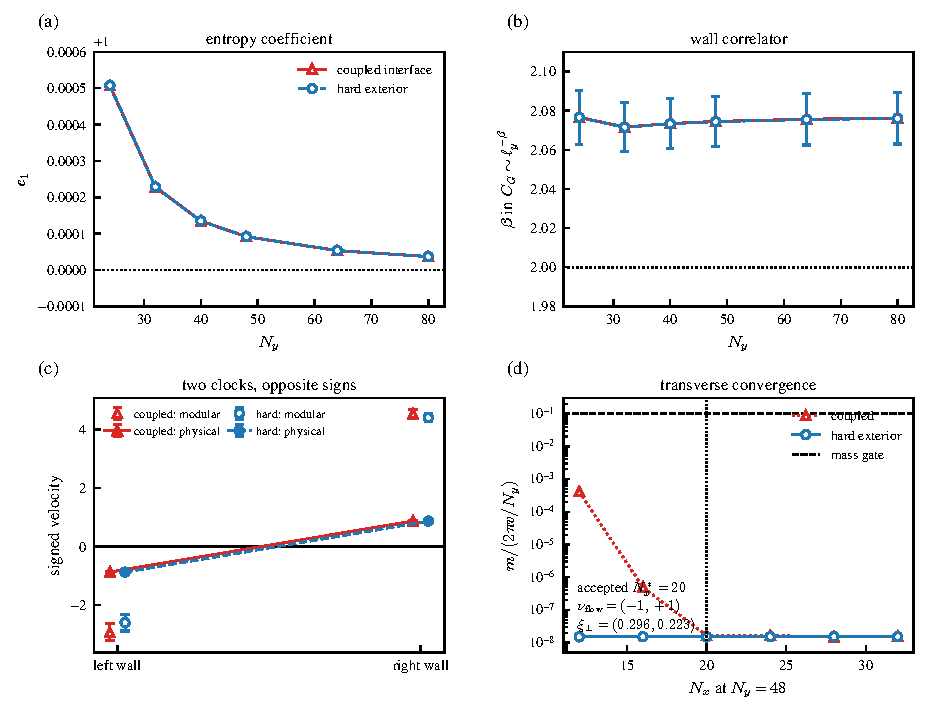
\includegraphics[width=0.98\linewidth]{result_01_exact_wall_benchmark.pdf}
\caption{\label{fig:exact-wall}Exact domain-wall calibration.  (a) Full-strip entropy
coefficient versus circumference, shown as $c$ near the $c=1$ target.  (b) Squared
wall-correlator exponent near the $r_y^{-2}$ target.  (c) Opposite physical and modular
velocities on the two walls; the magnitudes use different clocks and are not equated.
(d) Transverse convergence and the accepted $N_x=20$ gate.  Bars in (b) and (c) are
one-standard-error regression uncertainties; where absent visually, they are smaller than
the plotting symbols.  Panels (a) and (d) are deterministic diagnostics with no sampling
error bars.  The $20\times48$ accepted spectral projector is
$\Gamma_{\rm ex}=P_-(H_{\rm DW})$, equivalently the production covariance
$C_{\rm ex}=P_-^*(H_{\rm DW})$, from
Eqs.~\eqref{eq:real-space-hamiltonian}--\eqref{eq:exact-projector-convention};
panels (a)--(c) use Eqs.~\eqref{eq:entropy-target},
\eqref{eq:atlas-correlator-target}, and \eqref{eq:modular-velocity}.  This calibrates the
target and estimators, not adaptive preparation.}
\end{figure*}

\subsection{Result 2: a sharply localized slow tangent sector}

Figure~\ref{fig:tangent} places the two finite-time implementations and their selected-mode
localization on the same visual footing.
Two independent implementations give the same contrast.  In the CPU $T=2N_y$ campaign,
the wall gaps fall from $0.1125$ to $0.1014$ over $N_y=20,22,24$, while the uniform values
remain $0.894$--$0.896$.  The selected wall-sector weight is $0.992$--$0.996$.  In the GPU
$T=N_y$ campaign, the wall gaps are $0.02698(313)$, $0.02431(287)$, and $0.01968(225)$ at
$N_y=30,40,50$, compared with uniform gaps $0.7217(110)$, $0.7483(86)$, and $0.7676(87)$.
The corresponding slow-vector wall weights are $0.933$, $0.935$, and $0.944$.

Thus the important repeatable statement is not an absolute gap exponent: it is a
roughly eightfold CPU suppression, a $27$--$39$-fold GPU suppression, and strong spatial
localization in both data sets.  \evidence{canonical CPU and GPU finite-time precursors.}
\limittext{The campaigns use different clocks and trajectory suites, and neither is the
long-time $S=100$ production tangent family.}

\begin{figure*}[t]
\centering
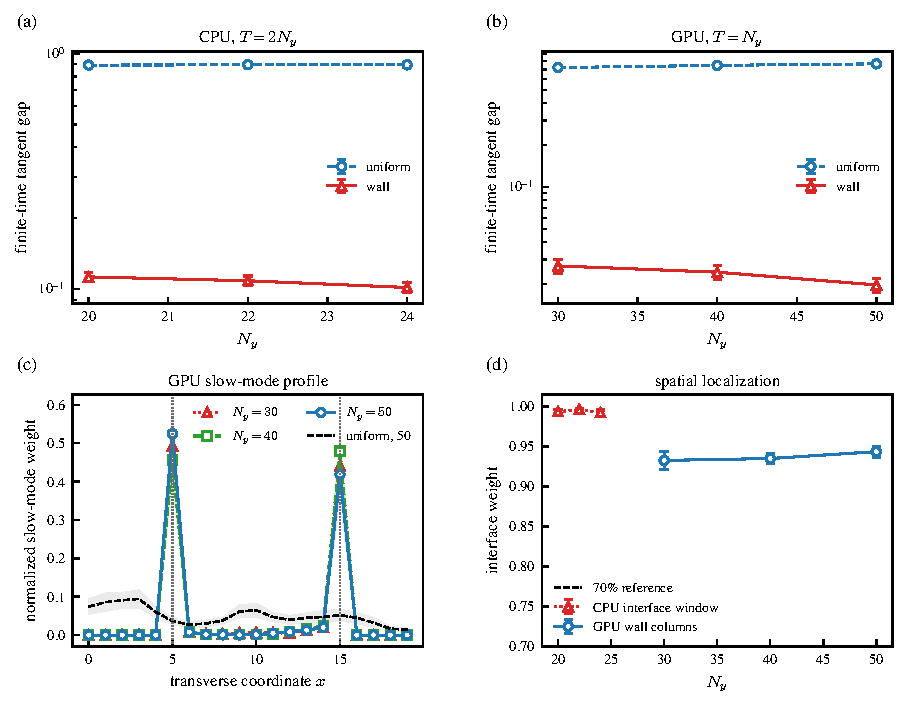
\includegraphics[width=0.98\linewidth]{result_02_tangent_slow_sector.pdf}
\caption{\label{fig:tangent}Wall-localized tangent sector.  (a) CPU wall and uniform
finite-time gaps.  (b) Independent GPU gaps on larger circumferences.  (c) GPU transverse
slow-mode profiles, with two peaks at the two interfaces.  (d) Integrated interface
weight for both campaigns; the black dashed line is a $70\%$ localization reference.
Bars in (a), (b), and (d), and shaded bands in (c), are trajectory standard errors for
$S=25$; several are smaller than the symbols or line width.  The CPU horizon is
$T=2N_y$ for $N_y=20,22,24$, whereas the GPU horizon is $T=N_y$ for
$N_y=30,40,50$.  Both are $N_x=20$, $n_{\rm shell}=1$, perfect-correction campaigns;
the wall arm has $(\alpha_{\rm in},\alpha_{\rm out})=(1,30)$,
\texttt{DW=True}, and \texttt{dw\_truncation=True}, while the uniform control has
$\alpha=1$, \texttt{DW=False}, and no wall truncation.  Both use the QR reduction in
Eq.~\eqref{eq:atlas-tangent-qr}.
Accordingly, the robust comparison is wall suppression and localization within each
campaign, not equality of their absolute finite-time rates.}
\end{figure*}

\subsection{Result 3: purification leaves a wall-localized residual}

Figure~\ref{fig:purification} collects the entropy, intrinsic charge variance, mass
control, and spatial-contour evidence for the surviving wall sector.
Starting from $C=\mathbf{1}/2$, the canonical $S=100$ GPU campaign rapidly removes the
extensive mixed-state entropy but leaves a finite residual at $2N_y$.  For
$N_y=30,40,50$, the final entropies are $0.2444(233)$, $0.2907(284)$, and $0.3313(271)$;
the charge variances are $0.06647(802)$, $0.08464(991)$, and $0.09733(952)$; and the
simultaneous Chern estimates remain $0.9891$, $0.9908$, and $0.9879$.  An independent
$16\times32$ contour archive places $94.25\%$ of the support-terminated final entropy on
the two wall columns.  The same smaller CPU sweep shows that a topological interior
$\alpha_{\rm in}=1$ retains orders of magnitude more entropy than the trivial
$\alpha_{\rm in}=3$ control.

\evidence{canonical ensemble dynamics plus a smaller spatial precursor.}
\limittext{No saved artifact contains the same record's full tangent cocycle and
purification spectrum, so the proposed recordwise tangent--purification bridge and a
universal purification exponent remain untested.  The principal ensemble stops at
$2N_y$.}

\begin{figure*}[t]
\centering
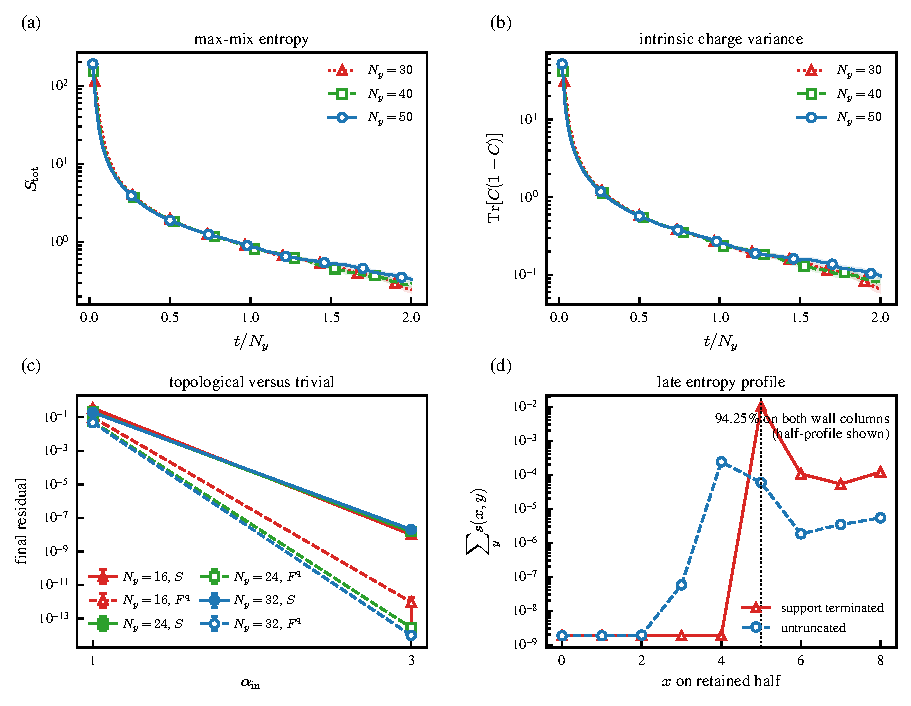
\includegraphics[width=0.98\linewidth]{result_03_purification_wall_residual.pdf}
\caption{\label{fig:purification}Max-mix purification.  (a) Total entropy and (b)
intrinsic charge variance collapse approximately with $t/N_y$ but retain a late residual.
(c) The residual strongly distinguishes the topological and trivial interiors in the CPU
mass sweep.  (d) A smaller contour archive localizes the late entropy to the wall; only
one half of the periodic transverse profile is displayed.  Bands in (a) and (b) are
$S=100$ trajectory standard errors, and bars in (c) are $S=10$ standard errors; many are
smaller than the curves or markers.  The contour export in (d) contains only its mean, so
no defensible recordwise error bar is available there.  The canonical panels use
$N_x=20$, $N_y=30,40,50$, $S=100$, and stop at $2N_y$; panel (d) is the separate
$16\times32$ archive.  Entropy, intrinsic variance, and contours are defined by
Eqs.~\eqref{eq:purification}, \eqref{eq:atlas-entropy}, and
\eqref{eq:atlas-contours}; the figure does not establish a purification exponent.}
\end{figure*}

\subsection{Result 4: logarithmic entropy is close to the two-wall \texorpdfstring{$c=1$}{c=1} value}

Figure~\ref{fig:entropy} shows the raw log-chord fit, its residuals, the size comparison,
and the cycle-resolved fitted coefficient.
The strongest common-depth entropy sequence uses $N_x=20$, $S=100$, $C=50$, and
$N_y=30,40,50$.  Fits over $A_y\geq8$ give the slopes
\begin{equation}
 m_1=0.35572(60),\quad 0.35092(58),\quad 0.34920(43),
\end{equation}
or, directly, $c_{\rm eff}=3m_1=1.0672(18),1.0528(17),1.0476(13)$, with
$R^2\geq0.99997$.  The discrepancy from $c=1$ decreases from $6.72\%$ to $4.76\%$
over this common sequence.  A separate time-scaled $S=10$, $C=N_y/2$ sequence gives
$c_{\rm eff}=1.08460(96),1.0665(13),1.05947(54)$ at $N_y=40,60,80$, and
$1.04098(42),1.0708(14)$ at $N_y=100,120$.  Because its depth and sample count differ,
it is displayed as a separate series rather than folded into the controlled extrapolation.  At
$20\times40$, $c_{\rm eff}(C)$ settles near $1.05$ after the early transient.

\evidence{canonical GPU $S=100$ state-entropy precursor plus the broader time-scaled
$S=10$ sequence.}
\limittext{The controlled $N_y=30$--$50$ trend is consistent with a $c=1$ two-wall state,
but it has a persistent positive finite-size/protocol bias and does not by itself establish
the current-algebra charge sector.}

\begin{figure*}[t]
\centering
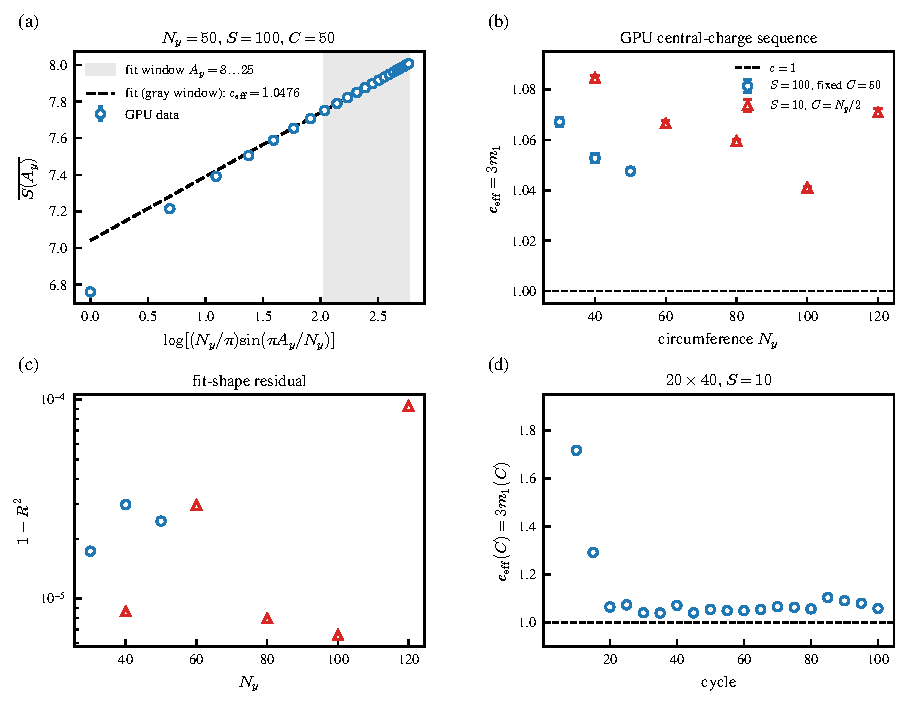
\includegraphics[width=0.98\linewidth]{result_04_entropy_log_chord.pdf}
\caption{\label{fig:entropy}Trajectory-averaged full-strip entropy.  (a) Raw log-chord
data for the largest controlled size.  The gray region is the actual fit window; empirical
points are unconnected, and the black dashed line extrapolates the fit across the displayed
range even though only $8\leq A_y\leq N_y/2=25$ points in the gray window enter the
regression.  (b) Direct GPU
$c_{\rm eff}=3m_1$ versus circumference for the fixed-$C$,
$S=100$ sequence and the separate time-scaled $S=10$ sequence.  Empirical points are not
connected; the dashed line is the $c=1$ target, not a fit.  (c) Fit residuals.
(d) $c_{\rm eff}(C)$ at $20\times40$, again without connecting empirical points.  Bars in
(a) are stored entropy standard errors; bars in (b) and (d) are one-standard-error fit
uncertainties.  Most are smaller than the symbols or line width.  The fixed-depth arm is
$N_x=20$, $S=100$, $C_{\rm cyc}=50$, $N_y=30,40,50$; the time-scaled arm has
$S=10$ and $C_{\rm cyc}=N_y/2$.  Equations~\eqref{eq:atlas-entropy} and
\eqref{eq:entropy-target} define the reduction.  The two arms are not combined into one
finite-size extrapolation.}
\end{figure*}

\subsection{Result 5: tripartite information counts one wall versus two}

Figure~\ref{fig:tmi} presents the raw exact and stochastic fits together with their
converted coefficients and symmetry-preserving fit-window sensitivity.
For full-width von Neumann entropies, the positive convention is
\begin{equation}
 \begin{aligned}
 \Delta I^{(\mathrm{full})}&\equiv I_2-I_3
 =I(A:C\mid B)\geq0,\\
 I_3-I_2&=-\Delta I^{(\mathrm{full})}.
 \end{aligned}
 \label{eq:tmi-sign-main}
\end{equation}
Here $I_2=I(A:C)$ and $I_3=I_3(A:B:C)$.  A one-wall datum is different: every subsystem
still spans the full transverse width, and only the final entanglement-contour sum is
restricted to a wall window $\mathcal X$.  Its plotted quantity is the algebraic contour
contribution
\begin{equation}
 \Delta I^{(\mathcal X)}=
 S_{AB}^{(\mathcal X)}+S_{BC}^{(\mathcal X)}
 -S_B^{(\mathcal X)}-S_{ABC}^{(\mathcal X)}.
 \label{eq:tmi-contour-main}
\end{equation}
It is not the entropy of a separately cut one-wall Hilbert space and is not, by itself, a
von Neumann conditional mutual information; strong subadditivity therefore constrains
only Eq.~\eqref{eq:tmi-sign-main}.  The wall curves are empirically positive, so the atlas
uses the same positive plotting orientation for both quantities.  Equations
\eqref{eq:tmi-definitions}--\eqref{eq:tmi-cft-fit} give the precise distinction and show
why both CFT reductions are linear in $z=\log[1/(1-x)]$.

The gray fit bands in Figs.~\ref{fig:tmi}(a) and \ref{fig:tmi}(b) do not mark ranges
selected afterward by fit quality.  Both source calculations used the conservative
periodic-geometry rule
\begin{equation}
 L_A+L_C\leq L_B\leq N_y-2(L_A+L_C),
 \label{eq:tmi-source-window}
\end{equation}
which requires both the intervening interval $B$ and the complementary interval
$D=N_y-(L_A+L_B+L_C)$ outside $ABC$ to have length at least $L_A+L_C$.  The rule avoids
either separation becoming the shortest scale and treats $B$ and $D$ symmetrically; it
was fixed by the generating notebooks, not optimized against these data.  Consequently,
panel (a) fits every stored $L_B=6,\ldots,28$ row and panel (b) every stored
$L_B=8,\ldots,15$ row.  Since the chord cross ratio is invariant under
$L_B\leftrightarrow D$ when $L_A=L_C$, symmetry-related rows can occupy the same displayed
$z$ coordinate.  The all-row fit remains the provenance-preserving baseline rather than a
window chosen to minimize $|c_{
m TMI}-1|$.

A symmetry-preserving sensitivity scan imposes the stronger rule $L_B,D\geq q$ and keeps
only fits with at least three distinct $z$ values.  For the exact data, increasing $q$ from
$6$ to $8$ changes $(c_{
m wall},c_{
m full})$ from
$(1.001806,1.002697)$ to $(1.000840,1.000922)$; at $q=11$ both are
$1.000464$ to the shown precision and the full/one-wall slope ratio is $2.0000003$.
This is the expected small short-distance correction, although the leverage and number of
distinct coordinates decrease as $q$ grows.  The historical stochastic result does not
behave as though its roughly $50\%$ excess came only from the endpoint rows.  It permits
only one nontrivial trim before fewer than three distinct coordinates remain: $q=9$ gives
$(c_{
m wall},c_{
m full})=(1.4748,1.5135)$ and ratio $2.0525$, compared with
$(1.4920,1.5335)$ and $2.0556$ at $q=8$.  The separate $L_A=L_C=3$ full-width fit falls
from $1.5754$ at $q=6$ to $1.4547$ at $q=10$, where only three distinct $z$ values remain.
Thus trimming improves the exact calibration and modestly lowers the stochastic
coefficients, but no defensible window makes the wrong-protocol stochastic pilot a
$c=1$ result.  The notebook diagnostic ledger records every accepted window and its
regression and whole-trajectory bootstrap uncertainties.

For the exact $20\times40$ ground state with $L_A=L_C=3$ and fixed $y_0=0$, the raw
contour-decomposed curves give slopes $0.166967668(27005)$ on each wall and
$0.334232464(95377)$ across the full width.  The full-to-one-wall ratio is $2.00178$, an
especially clean calibration of the $1/6$ and $1/3$ coefficients.  These fits imply
\begin{equation}
 \begin{aligned}
 c_{\rm TMI}^{\rm wall}&=6m=1.001806(162),\\
 c_{\rm TMI}^{\rm full}&=3m=1.002697(286),
 \end{aligned}
\end{equation}
which is one of the strongest numerical $c=1$ results in the repository.  The available
historical stochastic pilot uses $12\times31$, $C_{\rm cyc}=100$, $S=100$,
$L_A=L_C=4$, unwindowed OW modes, the legacy nonperfect
\texttt{dw\_symmetric} schedule, and the same full-subsystem/post-contour estimator.
Its trajectory-first curves give $0.2487(14)$ for one wall and $0.5112(14)$ for the
matched full window, a ratio $2.05549$, or $c_{\rm TMI}=1.4922(84)$ and $1.5336(42)$.
It therefore retains one-versus-two-wall counting while overshooting the central charge by
roughly $49\%$ and $53\%$; the separately archived $L_A=L_C=3$ full-window fit gives
$c_{\rm TMI}=1.5753(48)$.

For the stochastic raw curves, translated origins are averaged inside each trajectory
before the $S=100$ trajectory mean is formed, as in Eq.~\eqref{eq:trajectory-first-average}.
Pointwise bars are trajectory SEMs.  The quoted slope parentheses are ordinary regression
errors on the mean curve; a fixed-seed whole-trajectory bootstrap, which resamples the
100 records and repeats both the mean and fit, is retained separately as a correlated-fit
sensitivity check.  These three notions of uncertainty are not interchanged.

A separate block in \subfolder{notebooks/analysis.ipynb} contains stored trajectory-fit
outputs labeled $S=250$, but its present source sets \texttt{MAX\_SAMPLES\_MI=2}; its
embedded output is therefore stale relative to the executable cell.  It also uses a
$12\times16$, infinite-shell, old random-sequence reduced-strip estimator rather than the
full-width contour restriction above.  This is a source/output and estimator mismatch,
not superior production TMI evidence, so its coefficients are not promoted here.

\evidence{deterministic calibration and a provenance-recovered wrong-protocol stochastic
pilot.}  The exact and stochastic curve rows, geometry, averaging order, fit rows, and
source fingerprints are now machine-readable in the atlas-local cache rebuilt from their
generating calculation and covariance history.  \limittext{Recovering the raw curves does
not repair the stochastic protocol: it remains a one-size historical pilot with
unwindowed controller modes and nonperfect feedback, and is not production evidence for
the universal coefficient.}

\begin{figure*}[t]
\centering
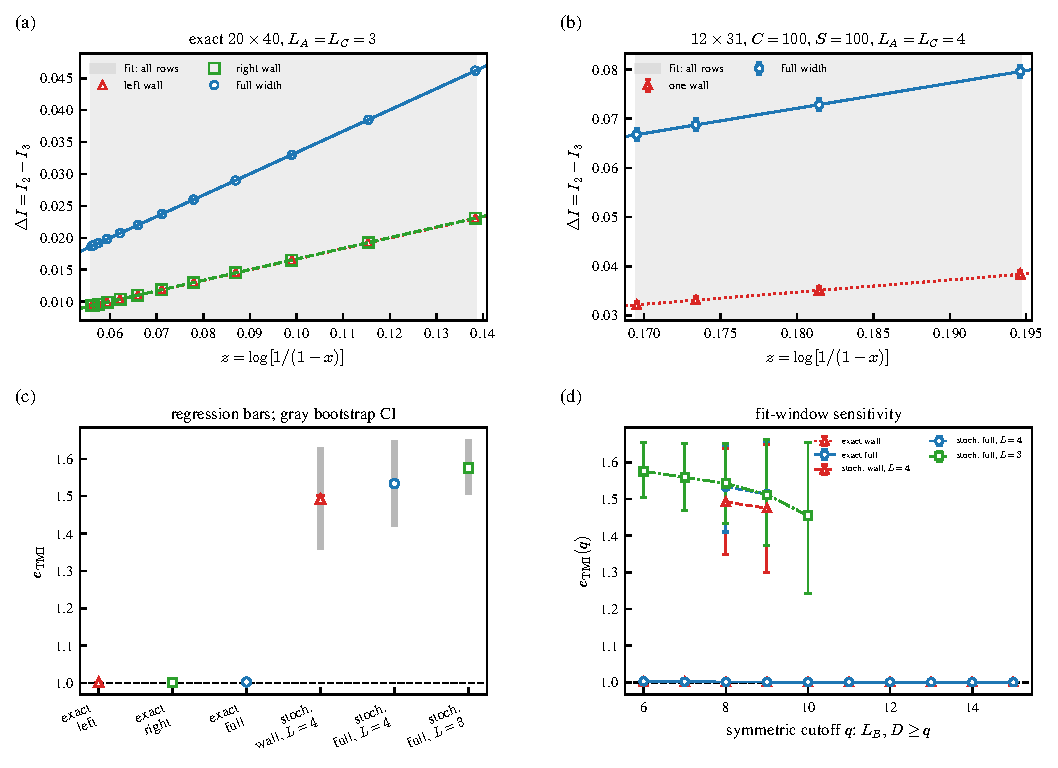
\includegraphics[width=0.98\linewidth]{result_05_tripartite_information.pdf}
\caption{\label{fig:tmi}Raw full-width conditional mutual information and one-wall
contour contributions.  The rigorous full-width quantity is
$\Delta I^{(\mathrm{full})}=I_2-I_3=I(A:C\mid B)\geq0$, so the requested
$I_3-I_2$ is its negative.  A wall curve is instead the algebraic post-contour
$\Delta I^{(\mathcal X)}$ in Eq.~\eqref{eq:tmi-contour-main}; it uses the same positive
plotting convention but is not itself a conditional mutual information.
(a) Exact $20\times40$ ground-state curves at $L_A=L_C=3$, $y_0=0$, for the left-wall,
right-wall, and full-$x$ post-contour sums.  Unconnected markers are measured values; the
gray band contains all stored $L_B=6,\ldots,28$ rows used in the regression, and each
fitted line is extended across the full displayed $z=\log[1/(1-x)]$ range.  There is no
trajectory sampling error.  This complete range is the source-era geometry rule in
Eq.~\eqref{eq:tmi-source-window}, not a residual- or fit-quality cut.
(b) Historical $12\times31$, $C_{\rm cyc}=100$, $S=100$, $L_A=L_C=4$ stochastic curves
for the matched wall and full-width estimator.  Origins are averaged within a trajectory
before the record mean; vertical bars are trajectory SEMs.  Lines fit all stored
$L_B=8,\ldots,15$ rows in the gray window and are not connections between points.  The
same Eq.~\eqref{eq:tmi-source-window} fixes this complete stored range; symmetry-related
$L_B$ and complementary-$D$ rows may coincide in $z$.  This arm uses
$n_{\rm shell}=\mathrm{None}$, nonperfect feedback, and the old
\texttt{dw\_symmetric} schedule.
(c) Exact and stochastic $c_{\rm TMI}$, using $6m$ for one wall and $3m$ for two walls;
the additional $L_A=L_C=3$ stochastic full-width fit is kept distinct.  Bars are
one-standard-error regression uncertainties.  The thick gray segments on the stochastic
points are fixed-seed $95\%$ whole-trajectory bootstrap intervals; they are also recorded
in the diagnostic ledger and are not substituted for the regression bars.
(d) Symmetry-preserving window scan imposing $L_B,D\geq q$ and retaining at least three
distinct $z$ values.  Exact bars are regression standard errors and are generally smaller
than the markers; stochastic bars are fixed-seed $95\%$ whole-trajectory bootstrap
intervals.  Trimming drives the exact coefficients still closer to one but only modestly
lowers the stochastic values.  The corresponding full/one-wall slope ratios remain
$2.0018\to2.0000$ exact and $2.0556\to2.0525$ stochastic over their accepted scans.
The stochastic result is an estimator pilot, not a production-protocol $c=1$
measurement.}
\end{figure*}

\subsection{Result 6: uniform trajectories approach the Chern-one target}

Figure~\ref{fig:chern} displays both the trajectory means and the individual final-state
spread of the real-space Chern estimator.
For uniform perfect-correction trajectories at $N_x=20$, $S=25$, and depths $C=N_y$,
the final real-space tripartition Chern means are
\begin{align}
 \overline{\mathcal{C}}_R&=0.9999950(23), &&N_y=30,\nonumber\\
 &=0.999687(298), &&N_y=40,\label{eq:chern-final}\\
 &=0.999927(60), &&N_y=50.\nonumber
\end{align}
where the parenthetical values are standard errors.  The lowest individual final value is
$0.992548$, occurring in the $N_y=40$ ensemble; the rest of the distributions cluster
tightly near unity.  This is the clearest adaptive bulk-topology precursor in the archive
and uses a Chern observable rather than a Bott index.

\evidence{canonical GPU trajectory precursor.}  \limittext{It is one radius-eight
real-space estimator on three finite rectangles and lacks the complete production suite
of marker profiles, purity-gap gates, and independent estimator cross-checks.}

\begin{figure*}[t]
\centering
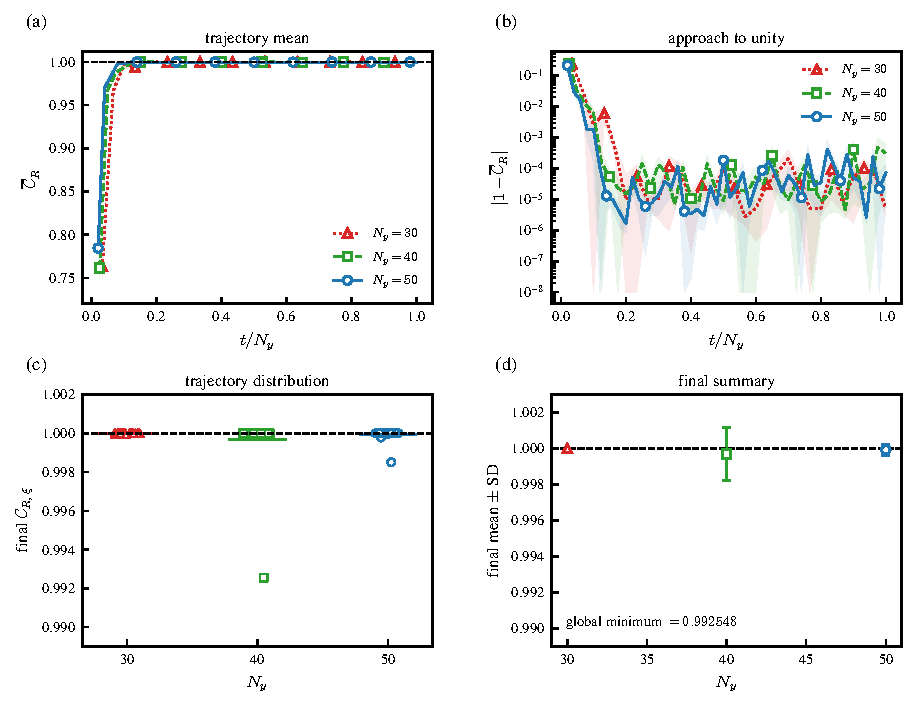
\includegraphics[width=0.98\linewidth]{result_06_uniform_topology.pdf}
\caption{\label{fig:chern}Uniform adaptive topology.  (a) Trajectory-mean real-space
Chern estimator.  (b) Absolute deviation from unity.  (c) Individual final-trajectory
values and ensemble means.  (d) Final means with standard-deviation bars, exposing the
single lower $N_y=40$ realization rather than hiding it in the mean.  Shaded bands in
(a) and (b) are trajectory standard errors for $S=25$ and are mostly smaller than the
lines; (d) deliberately uses standard deviations to display ensemble spread.  All panels
use uniform $N_x=20$, perfect-correction runs at $C_{\rm cyc}=N_y$ for
$N_y=30,40,50$ and the radius-eight estimator in
Eq.~\eqref{eq:atlas-tripartition-chern}.  This is one finite-radius topology precursor,
not a complete estimator cross-check.}
\end{figure*}

\section{Group II: feedback activity and the transition axis}

\subsection{Result 7: feedback activity is concentrated at the wall}

Figure~\ref{fig:activity} compares the spatial activity profile, integrated rates, and the
independently measured tangent-gap suppression.
The exact branchwise identity between the saved signed and absolute wrong-outcome
indicators is satisfied in the underlying activity archive.  At $N_y=24$, the transverse
profile has two sharp peaks at the wall locations, of order $0.09$ per update, while the
uniform background is a few $10^{-3}$.  Across $N_y=20,22,24$, the all-domain activity is
enhanced by factors $4.50$, $4.47$, and $4.84$ in the wall geometry.  Separately measured
tangent gaps are suppressed by factors $7.94$, $8.28$, and $8.83$ over the same sizes.

\evidence{canonical CPU finite-size precursor.}  \limittext{The activity and spectral
observables were obtained from separate trajectory suites.  Their coexistence supports a
mechanism hypothesis, but no recordwise activity--gap covariance, profile overlap,
matched purification residual, or causal statement is available.}

\begin{figure*}[t]
\centering
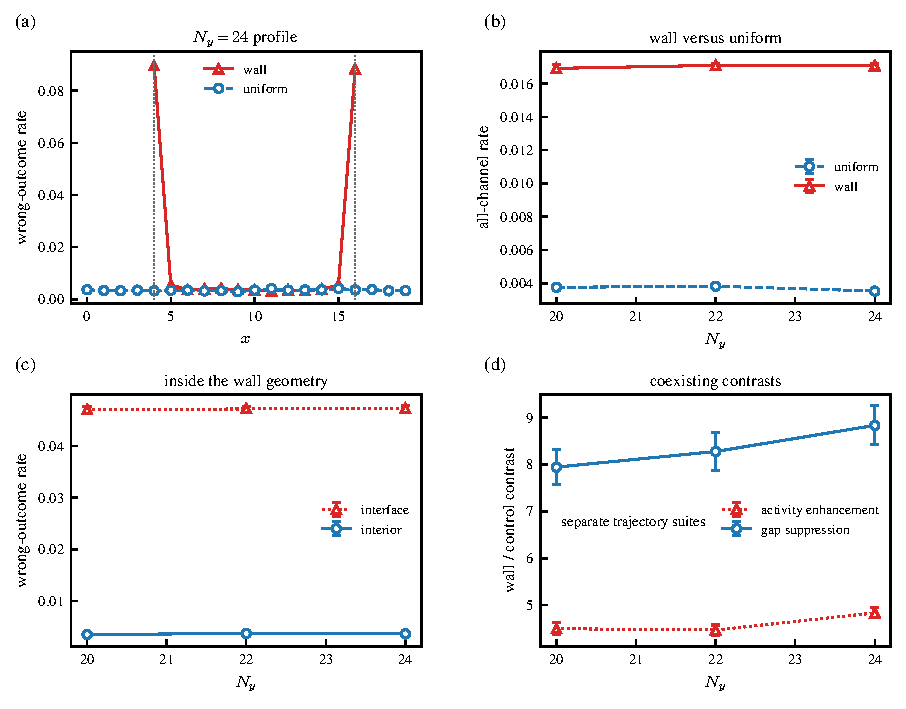
\includegraphics[width=0.98\linewidth]{result_07_feedback_activity.pdf}
\caption{\label{fig:activity}Born feedback activity.  (a) Two interface peaks in the
$N_y=24$ wall profile.  (b) Wall versus uniform all-domain rate.  (c) Interface and
interior rates within the wall geometry.  (d) Activity enhancement and independently
measured tangent-gap suppression; the annotation emphasizes that these are separate
trajectory suites.  The bands in (a) and bars in (b),(c) are trajectory standard errors
for $S=25$; (d) uses the corresponding propagated standard errors for each ratio.  Some
are smaller than the markers.  The $N_y=20,22,24$ CPU activity and tangent observables
use $N_x=20$, $S=25$, $C_{\rm cyc}=2N_y$, $n_{\rm shell}=1$, perfect correction, and a
raster-$y$ schedule.  The wall arm has $(\alpha_{\rm in},\alpha_{\rm out})=(1,30)$ and
\texttt{dw\_truncation=True}; the uniform control has $\alpha=1$ and no wall truncation.
They are computed by Eqs.~\eqref{eq:atlas-gaussian-measurement} and
\eqref{eq:atlas-tangent-qr}, but come from separate trajectory suites.  Panel (d)
therefore supports coexistence, not a recordwise activity--gap correlation.}
\end{figure*}

\subsection{Result 8: independent diagnostics change near \texorpdfstring{$\alpha=2$}{alpha=2}}

Figure~\ref{fig:alpha} places the particle--Choi and max-mix purification precursors on
the same mass axis while keeping their meanings separate.
The exact positive-mass transition lies at $\alpha_c=2$.  In the no-feedback GPU
particle--Choi proxy, the $N_y=20,30,40$ finite gaps at $\alpha=1.9$ are
$0.01215(229)$, $0.00808(182)$, and $0.00249(90)$, and all rise on the trivial side by
$\alpha=2.1$.  The perfect-correction proxy rises more sharply as $\alpha\to2^-$ and
loses finite samples at or above the transition; open points mark this censoring and a
missing finite sector is not converted into an infinite gap.  Independently, the CPU
max-mix scan at $N_y=32$ changes from entropy/variance $0.1244/0.03447$ at $\alpha=1.8$
to $0.002492/0.000309$ at $1.9$ and $2.0\times10^{-8}/7.9\times10^{-12}$ at $2.0$.

\evidence{canonical GPU transfer and CPU purification precursors.}
\limittext{The observables are not interchangeable: the transfer quantity is a
particle--Choi proxy and the CPU quantities describe transient max-mix purification.
There is no single saved stationary pure-state sweep containing topology, entropy,
charge, and tangent gates together.}

\begin{figure*}[t]
\centering
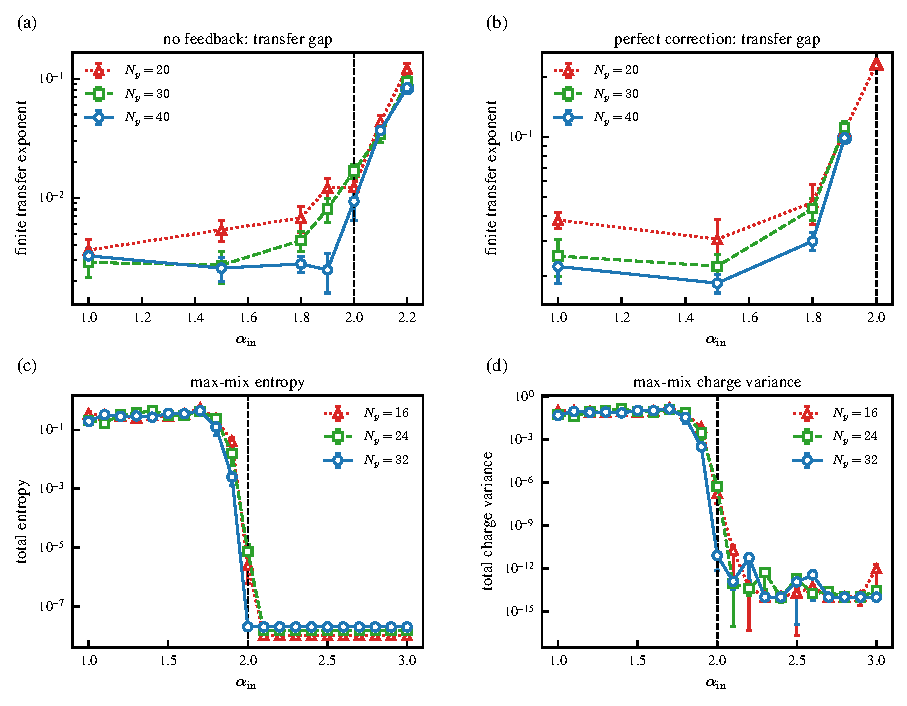
\includegraphics[width=0.98\linewidth]{result_08_alpha_transition.pdf}
\caption{\label{fig:alpha}Mass-transition precursors.  (a) No-feedback and (b)
perfect-correction finite transfer exponents.  Open overplotted markers denote censored
sample sets.  (c) Max-mix entropy and (d) max-mix charge variance from an independent CPU
sweep.  The vertical dashed line is the exact $\alpha_c=2$ transition.  Bars in (a),(b)
are standard errors over the finite transfer samples; bars in (c),(d) are $S=10$
trajectory standard errors.  Where not visible, they are smaller than the markers or
line width.  Panels (a,b) use $N_x=20$, $N_y=20,30,40$, $S=10$,
$C_{\rm cyc}=2N_y$, $n_{\rm shell}=1$, and \texttt{dw\_truncation=True}, comparing no
feedback with perfect correction.  Their reduced particle--Choi exponent and gap are
Eqs.~\eqref{eq:atlas-particle-choi} and \eqref{eq:atlas-particle-choi-exponents}.
Panels (c,d) use the independent $N_x=16$, $N_y=32$, $S=10$, $C_{\rm cyc}=2N_y$,
$n_{\rm shell}=1$, \texttt{dw\_truncation=True} perfect-correction max-mix covariance
and Eq.~\eqref{eq:purification}.  The two diagnostics are not
identified, and missing finite sectors are censoring rather than divergent gaps.}
\end{figure*}

\section{Group III: handedness and record observables}

\subsection{Result 9: modular flow has the orientation-dependent sign pattern}

Figure~\ref{fig:modular} shows the exact signed velocities and the corresponding
endpoint-resolved stochastic packet displacements.
The accepted B0 state gives modular velocities $(-2.930,+4.536)$ for the two walls, with
the same orientation reversal as the physical velocities.  A distinct observer applied
to stochastic trajectory covariances also gives the required endpoint-resolved signs.  At
$n_{\rm shell}=2$, the four final packet displacements are
\begin{equation}
 (8.821,-8.813,8.489,-8.520),
\end{equation}
where the sign alternates with packet endpoint and wall orientation according to the
stored labels.  The $n_{\rm shell}=1$ and $2$ observers agree on this pattern.

\evidence{completed exact handedness calibration plus a canonical stochastic precursor.}
\limittext{The stochastic data use translated cuts from a small number of trajectories;
those cuts are correlated variance-reduction samples, not independent records.  No
matched trivial modular controller or final $S=100$ accepted-size family exists, and
modular motion is not physical monitored-time transport.}

\begin{figure*}[t]
\centering
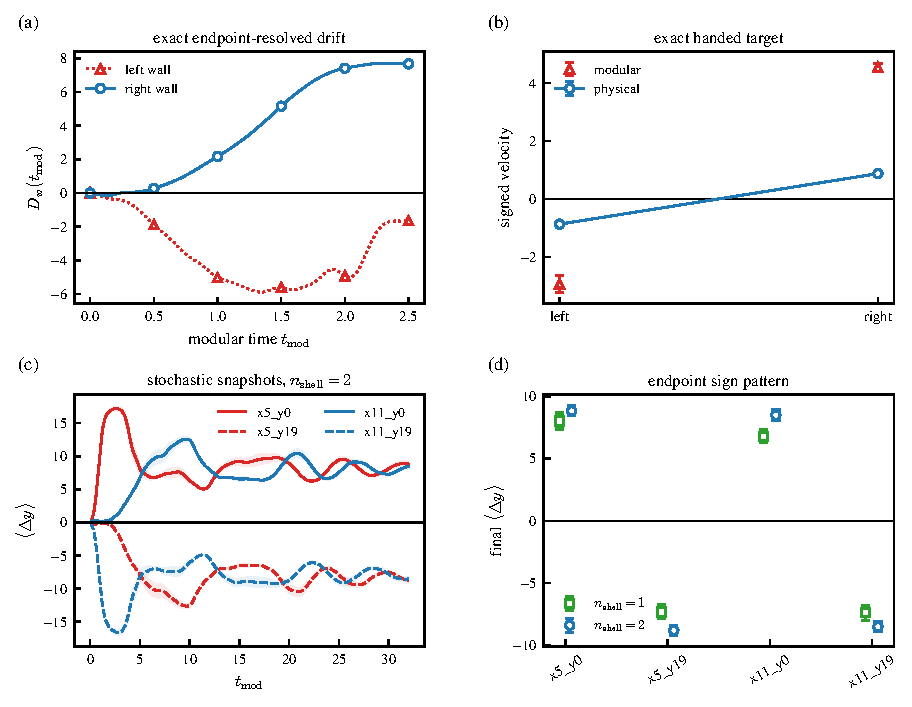
\includegraphics[width=0.98\linewidth]{result_09_modular_handedness.pdf}
\caption{\label{fig:modular}Modular handedness.  (a) Exact endpoint-resolved displacement.
(b) Exact modular and physical velocity signs.  (c) Stochastic packet trajectories for
$n_{\rm shell}=2$.  (d) Final endpoint sign pattern for two shell choices.  Bars in (b)
are regression standard errors; bands in (c) and bars in (d) are trajectory standard
errors after first averaging 40 translated origins within each of $S=10$ independent
records.  The superseded pooled-cut SEM is not plotted.  Several bars are smaller than
the curves or symbols; (a) is deterministic.  The stochastic panels use the cycle-50
$16\times40$ observer and the averaging order in
Eq.~\eqref{eq:trajectory-first-average}.  Equations~\eqref{eq:atlas-modular-generator}
and \eqref{eq:modular-velocity} define the motion; modular time is not the monitored
circuit clock.}
\end{figure*}

\subsection{Result 10: the classical probability record detects an active wall sector}

Figure~\ref{fig:record} displays the extensive chain entropy and its wall-resolved event
entropy density.
The probability maps retained by the streaming GPU campaigns determine
Eq.~\eqref{eq:record-entropy} even though the realized bits were not saved.  At late time,
the chain entropies per cycle are $89.6613(941)$, $119.7817(1013)$, and
$149.7625(1005)$ for $N_y=30,40,50$.  Dividing by $N_y$ gives
$2.98871(314)$, $2.99454(253)$, and $2.99525(201)$, showing a stable extensive
background.  At $20\times40$, the late binary entropy per event is $0.10129$ in the
distance-one wall neighborhoods and $0.01007$ elsewhere---a factor of about ten.

\evidence{canonical GPU chain-entropy feasibility result.}  \limittext{This is not an
individual record self-information, replica partition function, aspect-ratio scaling, or
record-CFT extraction.  It establishes that the archived classical probabilities contain
a sharply wall-enhanced uncertainty signal and motivates retaining complete record bits in
future runs.}

\begin{figure*}[t]
\centering
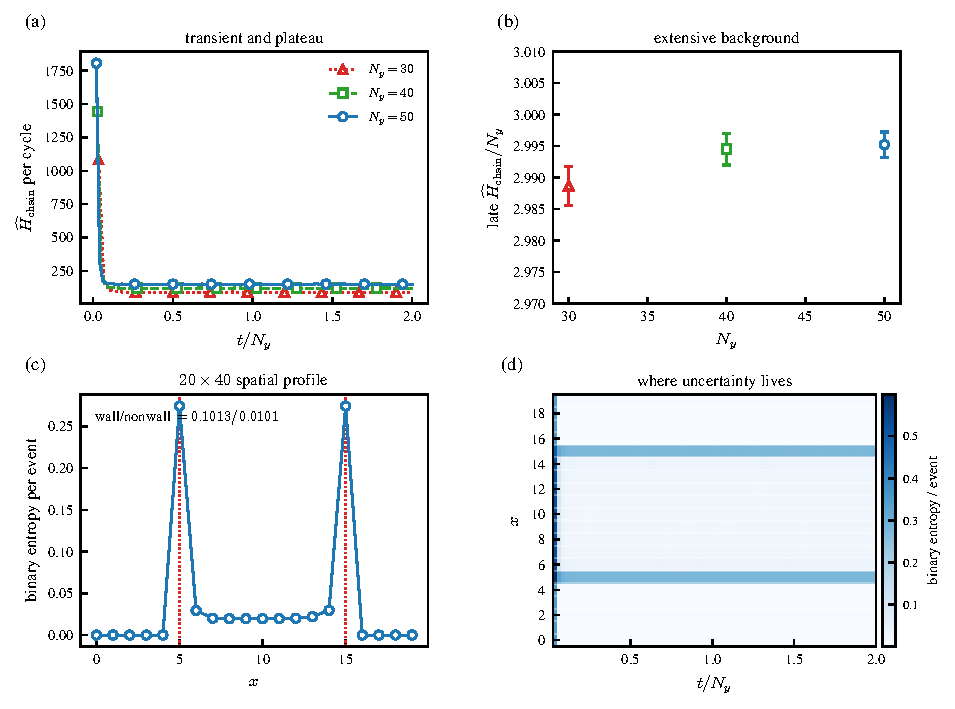
\includegraphics[width=0.98\linewidth]{result_10_record_uncertainty.pdf}
\caption{\label{fig:record}Classical probability-record uncertainty.  (a) Chain-entropy
transient and plateau.  (b) Late entropy divided by $N_y$.  (c) Late transverse profile at
$20\times40$.  (d) Space--time map using the BPJ-compatible sequential blue scale; the
two persistent high-uncertainty bands coincide with the walls.  The band in (a) and bars
in (b),(c) are trajectory standard errors for $S=100$; most are smaller than the line or
symbols.  Panel (d) is the ensemble-mean field and has no scalar error-bar overlay; its
fine white mesh marks individual transverse cells, with integer centers labeled every two
sites.  These $N_x=20$, $S=100$, $N_y=30,40,50$ streaming runs use the chain estimator
in Eq.~\eqref{eq:record-entropy}; panel (c) is the $20\times40$ late profile.  Because
outcome bits were not saved, none of the panels is a realized-record self-information or
a record-CFT coefficient.}
\end{figure*}

\section{Group IV: effective parents, spatial structure, and ensemble spread}

\subsection{Result 11: translation-resolved flattened spectra expose the wall modes}

The flattened-parent source notebook preserves translation symmetry along the periodic
direction and therefore decomposes the one-body problem into $k_y$ blocks.  The archived
spectrum shows the corresponding wall physics without first reducing it to a fitted
coefficient: the $X$- and $Y$-trial parents have especially clean counter-propagating
in-gap branches crossing zero, while the $Z$ trial retains the crossing within a more
structured bulk spectrum.  This is the spectral version of having two oppositely oriented
interfaces in a periodic transverse geometry.

\evidence{rendered deterministic flattened-Hamiltonian benchmark.}  The source notebook
and high-resolution PNG are both archived.  \limittext{The eigenvalue array itself was not
exported separately, so Fig.~\ref{fig:flat-spectrum} is a full-width crop of the legacy
render rather than a reconstruction from raw numeric rows.  It demonstrates visible
spectral flow but does not supply a new finite-size fit.}

\begin{figure*}[t]
\centering
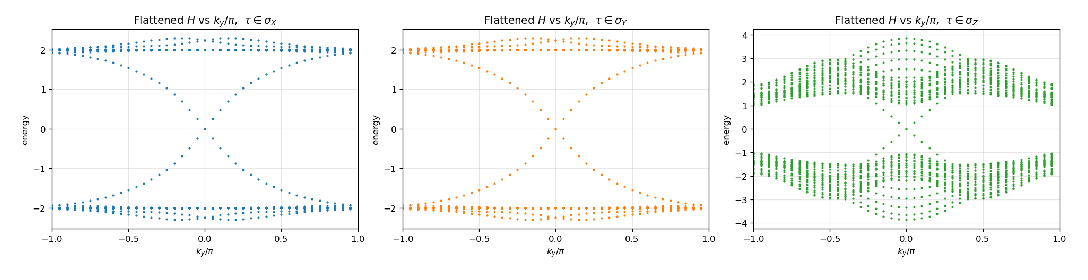
\includegraphics[width=0.98\linewidth]{result_11_flattened_wall_spectrum.pdf}
\caption{\label{fig:flat-spectrum}Translation-resolved flattened-parent spectra for the
$X$, $Y$, and $Z$ trial orbitals.  The $k_y$-resolved lower row of the archived benchmark
is given the full text width so the two in-gap wall branches and their zero-energy crossing
remain legible.  The source geometry is periodic $20\times40$ with
$(\alpha_{\rm in},\alpha_{\rm out})=(1,30)$ and $n_{\rm shell}=\mathrm{None}$; each
trial-orbital panel overlays \texttt{dw\_truncation=False} and true.  It is the
deterministic spectrum of Eq.~\eqref{eq:flat-parent} after
exact $y$-translation reduction, not a trajectory average; the plotted lower row is a crop
of the archived render because eigenvalue rows were not exported.  Visible spectral flow
is therefore preserved, but no new size fit or uncertainty is inferred.}
\end{figure*}

\subsection{Result 12: the finite-range uniform parent is already a gapped Chern insulator}

Figure~\ref{fig:flat-shells} compares the corrected uniform-parent Chern response, gap,
and the separate domain-wall entropy and correlator diagnostics across shell depth.
The flattened-parent bulk topology must be tested in a uniform gapped geometry, not with
a tripartition disk that intersects both sides of a domain wall.  Direct reconstruction at
$20\times40$ gives
\begin{equation}
\begin{array}{c|cc|c}
n_{\rm shell} & \mathcal C_R(\alpha=1) & \mathcal C_R(\alpha=3)
& \min|E|(\alpha=1)\\ \hline
0 & 0 & 0 & 1.582825\\
1 & -0.999999829 & -2.82\times10^{-8} & 1.802517\\
2 & -0.999997053 & -5.46\times10^{-7} & 1.902787\\
\mathrm{full} & -0.999942295 & -1.30\times10^{-5} & 2.000000
\end{array}
\label{eq:uniform-flat-parent-topology}
\end{equation}
for the $X$-trial construction.  An independent momentum-space FHS evaluation of the
$n_{\rm shell}=1$ lower band gives $C_{\rm FHS}=-1$ at $\alpha=1$ and zero at
$\alpha=3$; the real-space calculation now evaluates that same occupied projector and
agrees, $\mathcal C_R=-0.999999829$ and $-2.82\times10^{-8}$, respectively.  Thus its
sign is not produced by a complementary-band substitution.  It is the raw flattened-frame
orientation, which is opposite the $C=+1$ spectral-projector orientation used for the
exact Hamiltonian and form-factor sweep.  The $n_{\rm shell}=1$ occupied band has width
$0.386523$, so
``flattened parent'' does not mean an exactly flat finite-range Chern band.

The separate domain-wall tables answer a different convergence question.  With
domain-wall truncation, one shell already gives the two-wall and one-wall entropy slopes
$0.333983$ and $0.166750$, close to $1/3$ and $1/6$, while the wall-correlator exponent is
$3.20326$.  Two shells give $3.15179$, and full support gives $2.00421$.  The formerly
quoted finite-domain-wall Chern scalar is excluded here because its radius-eight
tripartition disk, centered at $x=10$, crosses the interfaces at $x=6,14$ and is not a
uniform bulk invariant.  Thus finite support already preserves the uniform bulk topology;
the slower shell convergence belongs to the domain-wall correlator tail.

Equations~\eqref{eq:flat-parent} and \eqref{eq:ky-fan-loss} also make precise the relation
to Ky Fan optimization: filling the lowest parent eigenstates minimizes the simultaneous
\emph{additive} penalty for undesired local outcomes.  It does not maximize a single joint
probability for mutually overlapping measurements.

\evidence{direct deterministic reconstruction of the uniform flattened parent from the
canonical CPU implementation, independently checked by real-space tripartition and
momentum-space FHS topology; machine-readable domain-wall entropy and correlator tables.}
\limittext{This benchmark characterizes an effective static parent and its ground state;
it does not prove that finite-depth adaptive dynamics samples that state exactly.  The
uniform FHS integer is not assigned to the globally gapless domain-wall geometry.}

\begin{figure*}[t]
\centering
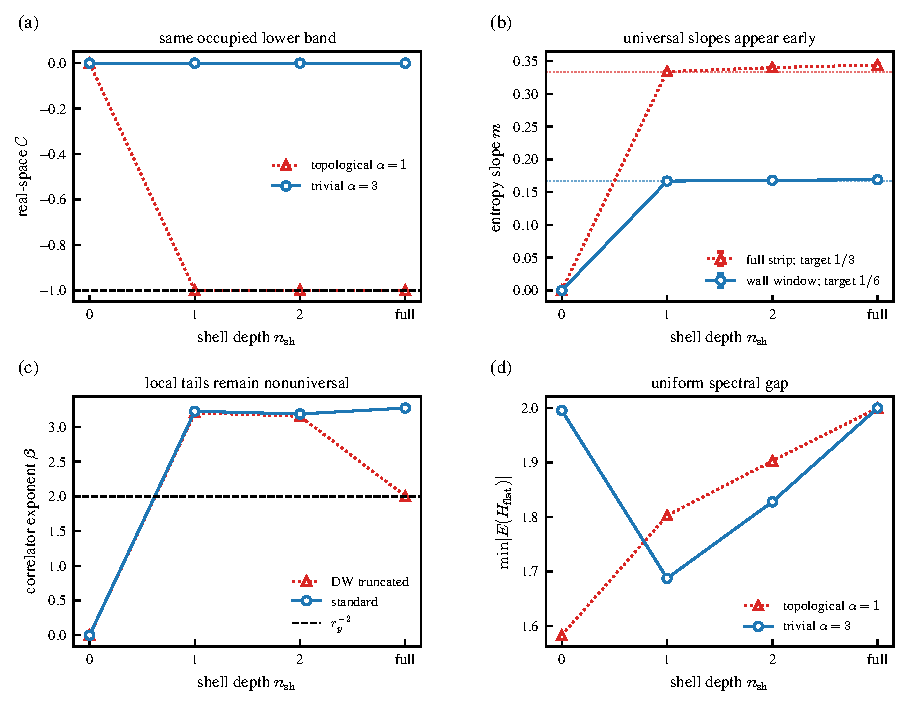
\includegraphics[width=0.98\linewidth]{result_12_flattened_shell_benchmark.pdf}
\caption{\label{fig:flat-shells}Corrected flattened-parent audit.  (a) Uniform real-space
Chern response for the topological $\alpha=1$ parent and trivial $\alpha=3$ control.
The independent $n_{\rm shell}=1$ lower-band FHS integers are $-1$ and zero, respectively;
the real-space tripartition routine evaluates the same occupied projector and agrees in
sign and magnitude.  (b) Full-strip and
wall-window entropy coefficients in the separate domain-wall construction.  (c) Its
wall-correlator exponent.  (d) Uniform distance of the flattened-parent spectrum from
zero.  ``Full'' means the untruncated shell sum.  Bars in (b) are the RMS
one-standard-error regression uncertainty across the contributing interval fits and are
generally smaller than the markers.  The remaining panels are deterministic, so sampling
error bars do not apply.  The uniform panels use $20\times40$ and
Eqs.~\eqref{eq:atlas-tripartition-chern}, \eqref{eq:atlas-fhs}, and
\eqref{eq:atlas-ky-fan}; the entropy/correlator panels belong to a separate domain-wall
construction governed by Eqs.~\eqref{eq:entropy-target} and
\eqref{eq:atlas-correlator-target}.  Static-parent topology is not finite-depth adaptive
preparation.}
\end{figure*}

\subsection{Result 13: spatial maps resolve the wall rather than a featureless bulk}

Four complementary maps in Fig.~\ref{fig:spatial-maps} make the geometry visible.  The
exact local Chern marker is uniform in the topological strip and switches across its
interfaces.  The $S=25$ slow-vector density is concentrated at the two wall columns.  An
independent $S=10$ half-strip entanglement contour at circuit cycle $50$ is similarly
wall-centered, and the $S=100$ max-mix charge-variance map at $2N_y$ shows where residual
purification noise lives.  These fields are particularly useful guards against a scalar
average being produced by a diffuse bulk background.

\evidence{one rendered exact calibration and three machine-readable adaptive maps.}
\limittext{The adaptive panels use different accepted precursor campaigns and sizes.  They
show mutually compatible localization, not a recordwise equality between tangent,
entanglement, and charge fluctuations.}

\begin{figure*}[t]
\centering
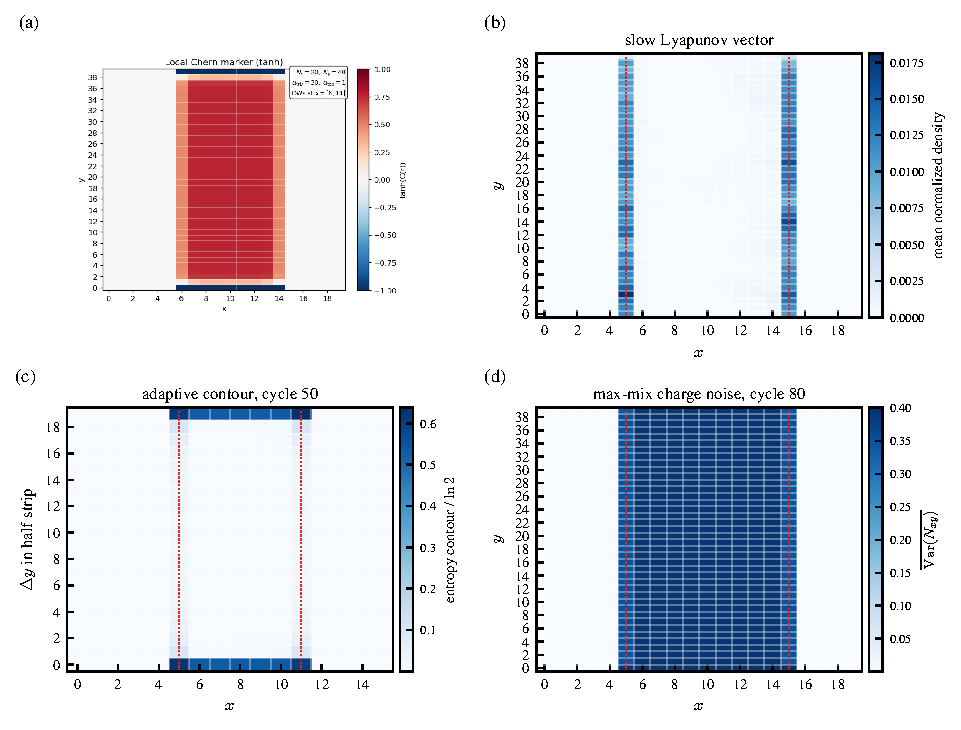
\includegraphics[width=0.98\linewidth]{result_13_spatial_evidence_maps.pdf}
\caption{\label{fig:spatial-maps}Spatial evidence.  (a) Archived exact local-Chern render;
the numeric field was not separately exported.  (b) Ensemble-averaged density of the
minimum-absolute Lyapunov vector at $20\times40$.  (c) Final $16\times40$ half-strip
entanglement contour.  (d) Final $20\times40$ max-mix local charge variance.  Dotted red
lines mark the wall columns in the machine-readable adaptive panels.  The fine white mesh
delineates every unit cell, with integer centers labeled every two sites.  Panels (a)--(d)
respectively use Eqs.~\eqref{eq:atlas-local-chern}, \eqref{eq:atlas-tangent-qr}, and
\eqref{eq:atlas-contours}; the adaptive inputs have $S=25$, $S=10$ at cycle 50, and
$S=100$ at $2N_y$, respectively.  Their compatible localization does not make them
recordwise paired observables.}
\end{figure*}

\subsection{Result 14: modular propagation is visible before center-of-mass reduction}

The signed displacements in Result 9 are reductions of a much richer density movie.
Figure~\ref{fig:modular-maps} shows four snapshots from the cycle-$50$, sample- and
origin-averaged modular evolution at $16\times40$.  The initially localized charge packet
redistributes through the half-strip while retaining pronounced structure tied to the two
wall columns.  This provides a direct spatial check on the endpoint-resolved sign analysis
without confusing modular time with monitored circuit time.

\evidence{canonical CPU observer applied to $S=10$ GPU covariance snapshots.}
\limittext{The origin translations are correlated variance-reduction samples, and this is
not a real-time charge response or a matched trivial control.}

\begin{figure*}[t]
\centering
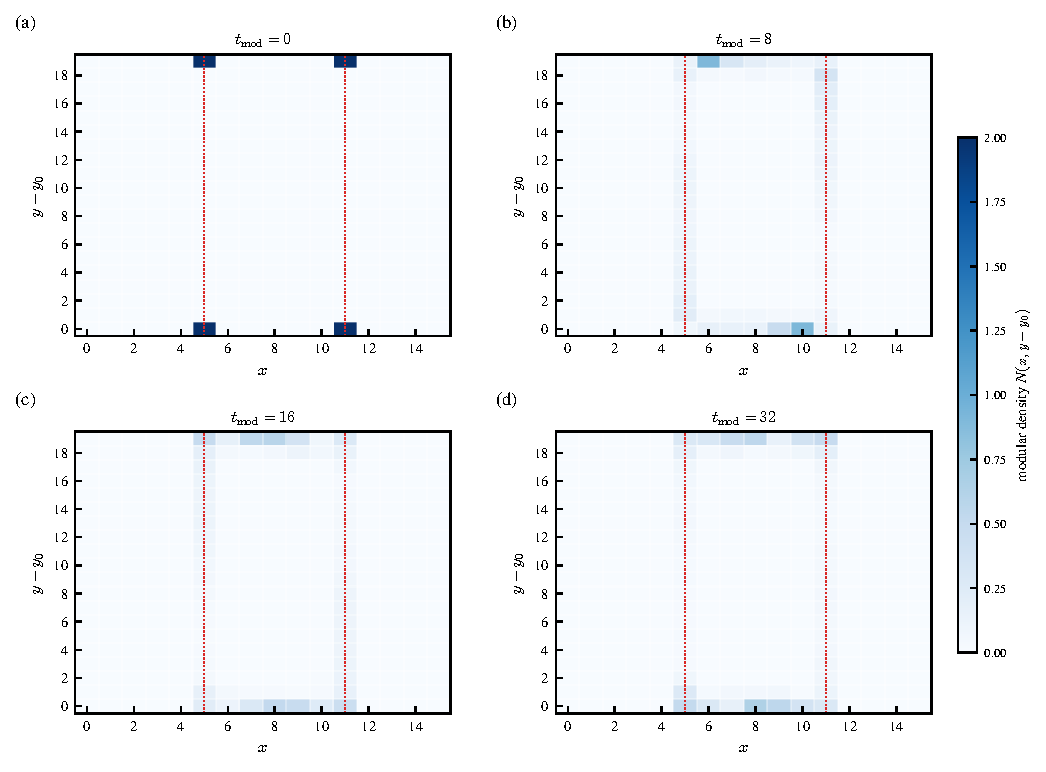
\includegraphics[width=0.98\linewidth]{result_14_modular_density_heatmaps.pdf}
\caption{\label{fig:modular-maps}Modular charge-density snapshots at
$t_{\rm mod}=0,8,16,32$.  The horizontal coordinate is the physical transverse direction;
the vertical coordinate is the periodic position relative to the half-strip origin.
Red dotted lines mark the two domain walls; the fine white mesh delineates individual unit
cells, with integer centers labeled every two sites.  These are cycle-50,
$16\times40$, $S=10$ covariance snapshots propagated by
Eq.~\eqref{eq:atlas-modular-generator}, with translated origins averaged within each
record before the ensemble mean.  They visualize modular, not physical-time, density
propagation and carry no independent scalar error overlay.}
\end{figure*}

\subsection{Result 15: typical trajectories cluster near the target, but tails remain}

The shared final-cycle features used in Results 15 and 16 are defined from the local
cell occupation $q_\xi(x,y)=\sum_\mu C_{\xi,(x,y,\mu),(x,y,\mu)}$ and
$Q_\xi=\sum_{x,y}q_\xi(x,y)$ by
\begin{align}
 d_{Q,\xi}&=100\frac{|Q_\xi-N_xN_y|}{N_xN_y},
 &d_{\mathcal C,\xi}&=|\mathcal C_{R,\xi}-1|,\nonumber\\
 r_{{\rm wall},\xi}
 &=\left[\frac1{|\mathcal W|}
 \sum_{(x,y)\in\mathcal W}q_\xi(x,y)^2\right]^{1/2}.
 \label{eq:trajectory-quality-metrics}
\end{align}
Here $\mathcal W$ contains all $y$ and the five columns within radius two of either wall,
exactly as in the saved feature table.  Thus ``wall-charge RMS'' is an RMS of the local
cell occupation, not an RMS of the globally centered filling.

The $C_{\rm cyc}=2N_y$ distributions in Fig.~\ref{fig:distributions} replace a vague claim of
ensemble cleanliness with a record-resolved statement.  Across $S=100$ trajectories, the
means of $c_{\rm eff}=3m_s$ are $1.0794$, $1.0476$, and $1.0436$ at
$N_y=30,40,50$; the corresponding standard deviations are $0.0894$, $0.0350$, and
$0.0364$.  The real-space Chern medians are $0.9993$, $0.9978$, and $0.9983$, although
rare records extend down to $0.433$, $0.623$, and $0.617$.  Charge drift remains discrete
and decreases with circumference.  Independently, final max-mix $V_Q$ is broad and
right-skewed: its medians are $0.0304$, $0.0357$, and $0.0573$, well below its means
$0.0665$, $0.0846$, and $0.0973$.

\evidence{canonical $S=100$ trajectory-resolved pure-state and purification diagnostics.}
\limittext{The typical records support near-$c=1$, near-unit-Chern behavior, but the tails
rule out saying that all records are equivalent.  The pure-state and max-mix histograms
come from separate ensembles and are not paired trajectory by trajectory.}

\begin{figure*}[t]
\centering
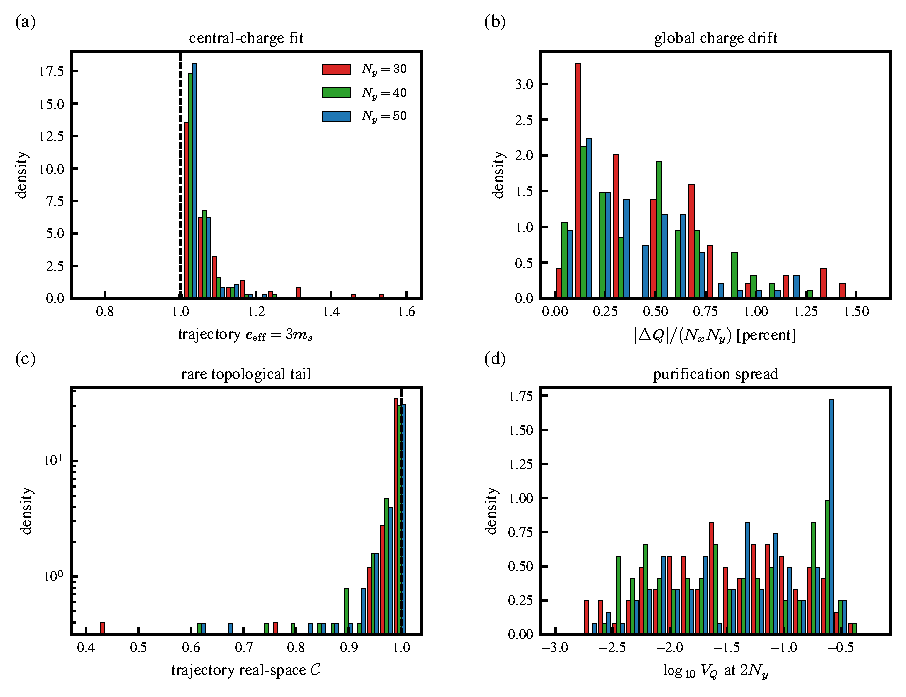
\includegraphics[width=0.98\linewidth]{result_15_trajectory_distributions.pdf}
\caption{\label{fig:distributions}Trajectory distributions at $C_{\rm cyc}=2N_y$: cycles
$C_{\rm cyc}=60,80,100$ for $N_y=30,40,50$, respectively.  (a) Effective central charge from the
per-trajectory entropy slope.
(b) Absolute global charge drift.  (c) Real-space Chern response on a logarithmic density
axis to expose rare low-Chern records.  (d) Final intrinsic charge variance during max-mix
purification.  All panels use side-by-side filled histogram bars with narrow inter-bin
spacing and black outlines; colors identify circumference as in the legend.  Each bar
sample is one trajectory scalar from $S=100$ at $N_x=20$, with cycles
$60,80,100$ for $N_y=30,40,50$.  Panels (a--d) use
Eqs.~\eqref{eq:entropy-target}, \eqref{eq:trajectory-quality-metrics},
\eqref{eq:atlas-tripartition-chern}, and \eqref{eq:purification}.  The pure-state arm is
perfect correction with $n_{\rm shell}=1$ and \texttt{dw\_truncation=True}; pure-state
and max-mix records are separate ensembles.  The histograms carry no separate error bars;
their recordwise spread is the displayed distribution.  The
tails preclude an all-records-equivalent claim.}
\end{figure*}

\subsection{Result 16: ensemble cleaning is observable-dependent}

Figure~\ref{fig:cleaning} shows how the inferred coefficient changes under each declared
trajectory-ranking functional and retained fraction.
Post hoc rank conditioning does not produce a unique ``clean'' ensemble.  Retaining the
smallest global charge drifts can leave the central-charge excess unchanged or even worsen
it, especially at $N_y=30$.  Conditioning on wall-charge RMS or Chern error reduces the
excess for some circumferences and retained fractions, but the behavior is not uniform.
The aggressive $10\%$ points contain only ten records and carry correspondingly larger
uncertainty.  Any future cleaning rule must therefore be preregistered, report its retained
fraction, and be checked against multiple independent observables.

\evidence{post hoc diagnostic on the canonical $S=100$ final-cycle feature table.}
\limittext{This is a sensitivity analysis, not a production reweighted ensemble and not
evidence that unfavorable trajectories should be discarded.}

\begin{figure*}[t]
\centering
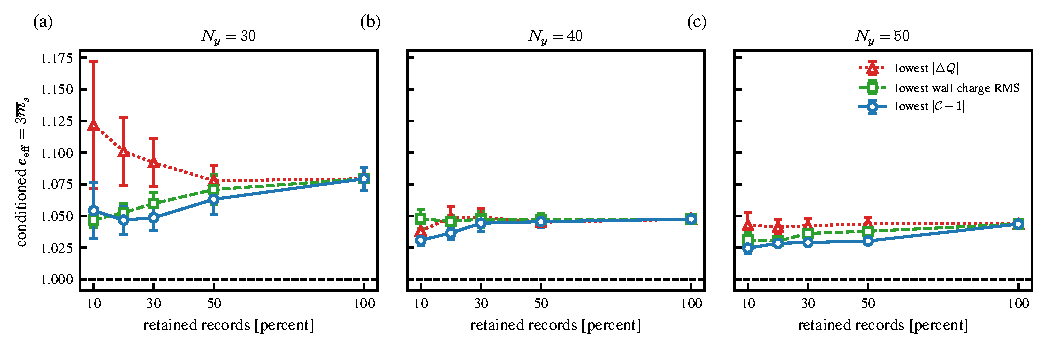
\includegraphics[width=0.98\linewidth]{result_16_ensemble_cleaning_sensitivity.pdf}
\caption{\label{fig:cleaning}Conditioned effective central charge versus retained record
fraction.  Each panel fixes a circumference; curves rank trajectories by global charge
drift, wall-charge RMS, or real-space Chern error.  Error bars are standard errors of the
retained subset (some are smaller than the markers), and the dashed line is $c=1$.
Every point is an unweighted recomputation from the $S=100$ final-cycle feature table
after retaining the displayed rank fraction, with uncertainty defined by
Eqs.~\eqref{eq:trajectory-quality-metrics} and \eqref{eq:atlas-sem}.  The table uses
$N_x=20$, $N_y=30,40,50$, $C_{\rm cyc}=2N_y$, $n_{\rm shell}=1$,
\texttt{dw\_truncation=True}, and perfect correction.  This is a post hoc sensitivity
analysis, not partial
post-selection or a redefined physical ensemble.}
\end{figure*}

\subsection{Result 17: the filling distribution narrows with circumference}

Figure~\ref{fig:filling-variance} gives the cycle-resolved population variance and its
final-size comparison for both saved preparations.
The final-cycle charge-drift histogram in Result 15 hides a useful finite-size fact.
For each record $\xi$, define the centered filling deviation in percentage points by
\begin{equation}
 \begin{aligned}
 \delta\nu_\xi(C_{\rm cyc})
 &=100\frac{Q_\xi(C_{\rm cyc})-N_xN_y}{N_xN_y},\\
 \sigma_\nu^2(C_{\rm cyc})
 &=\operatorname{Var}_\xi[\delta\nu_\xi(C_{\rm cyc})].
 \end{aligned}
 \label{eq:filling-variance}
\end{equation}
The raw cell-charge histories show the same narrowing in two independent $S=100$
campaigns.  At $C_{\rm cyc}=2N_y$, the pure-state variances are
$0.29684$, $0.21614$, and $0.16534$ squared percentage points for
$N_y=30,40,50$; the max-mix purification values are $0.28533$, $0.20166$, and
$0.17023$.  Thus the $N_y=30\to50$ reduction is $44.3\%$ and $40.3\%$, respectively.
The corresponding standard deviations narrow from $0.545$ to $0.407$ and from $0.534$
to $0.413$ percentage points.  Agreement between the two preparations makes the trend
more credible than either archive alone, although three sizes do not determine an
asymptotic exponent.

\evidence{two canonical $S=100$, $N_x=20$ trajectory-resolved charge campaigns.}
\limittext{$\sigma_\nu^2$ is sample-to-sample variance of normalized total filling, not
the within-trajectory quantum variance $V_Q=\langle Q^2\rangle-\langle Q\rangle^2$ and
not proof that every trajectory is identical.}

\begin{figure*}[t]
\centering
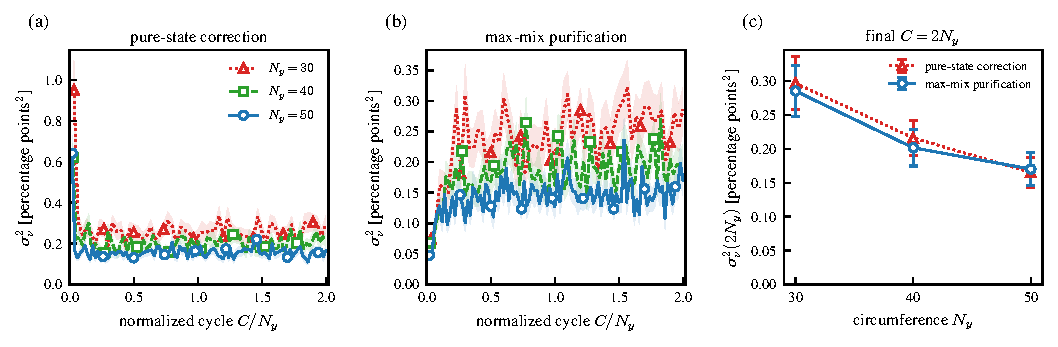
\includegraphics[width=0.98\linewidth]{result_17_filling_variance_scaling.pdf}
\caption{\label{fig:filling-variance}Trajectory-to-trajectory filling variance.
(a) Pure-state perfect correction and (b) maximally mixed purification versus normalized
cycle $C_{\rm cyc}/N_y$.  Curves show the population variance across $S=100$ records; translucent
bands are leave-one-record-out jackknife standard errors and can be narrower than the
lines.  (c) Final values at $C_{\rm cyc}=2N_y$, i.e., cycles $60,80,100$ for
$N_y=30,40,50$.  Error bars are the same jackknife standard errors from
Eqs.~\eqref{eq:filling-variance} and \eqref{eq:atlas-jackknife}.  Both preparations use
$N_x=20$, $S=100$, $n_{\rm shell}=1$, \texttt{dw\_truncation=True}, and perfect
correction; the plotted
quantity is the population variance of normalized trajectory filling, not the intrinsic
quantum variance in Eq.~\eqref{eq:atlas-charge-cumulants}, and three sizes do not fix an
asymptotic exponent.}
\end{figure*}

\subsection{Result 18: an independent pure-state archive checks entropy and correlations}

The Colab audit found a second physical-state archive that had not been represented in the
atlas.  Canonical perfect-correction covariance snapshots at $N_x=16$, $N_y=30,40$,
$n_{\rm shell}=1,2$, $S=10$, and $C=50$ support both entropy and correlation analyses.
The late-window full-width fits give
\begin{equation}
\begin{array}{c|cc}
 & n_{\rm shell}=1 & n_{\rm shell}=2\\ \hline
N_y=30 & c_{\rm eff}=1.04583(13) & 1.05513(16)\\
N_y=40 & c_{\rm eff}=1.03244(22) & 1.08650(21),
\end{array}
\end{equation}
with $R^2\geq0.99995$.  The quoted entropy uncertainties are regression standard errors
over the fit points, not trajectory errors.  On the declared correlator window
$2\leq r_y\leq N_y/4$, the two-wall-window exponents are $2.154(36)$, $2.126(33)$,
$2.191(36)$, and $2.092(34)$ in the same order; the nonwall controls instead lie between
$4.11$ and $6.37$.  Thus the archive independently supports a wall-localized algebraic
sector at both shell depths.  The endpoint map in Fig.~\ref{fig:small-state-crosscheck}(c)
also makes the limitation visible: the numerical exponent moves substantially under
arbitrary endpoint choices, so this remains a selected-window cross-check rather than a
precision universal-exponent determination.

\evidence{canonical $S=10$ perfect-correction covariance snapshots with independent
entropy and correlator analyses.}
\limittext{Only two circumferences are present.  A high $R^2$ at one declared window does
not remove the explicit fit-window sensitivity, and the regression errors are not a
whole-trajectory finite-size uncertainty.}

\begin{figure*}[t]
\centering
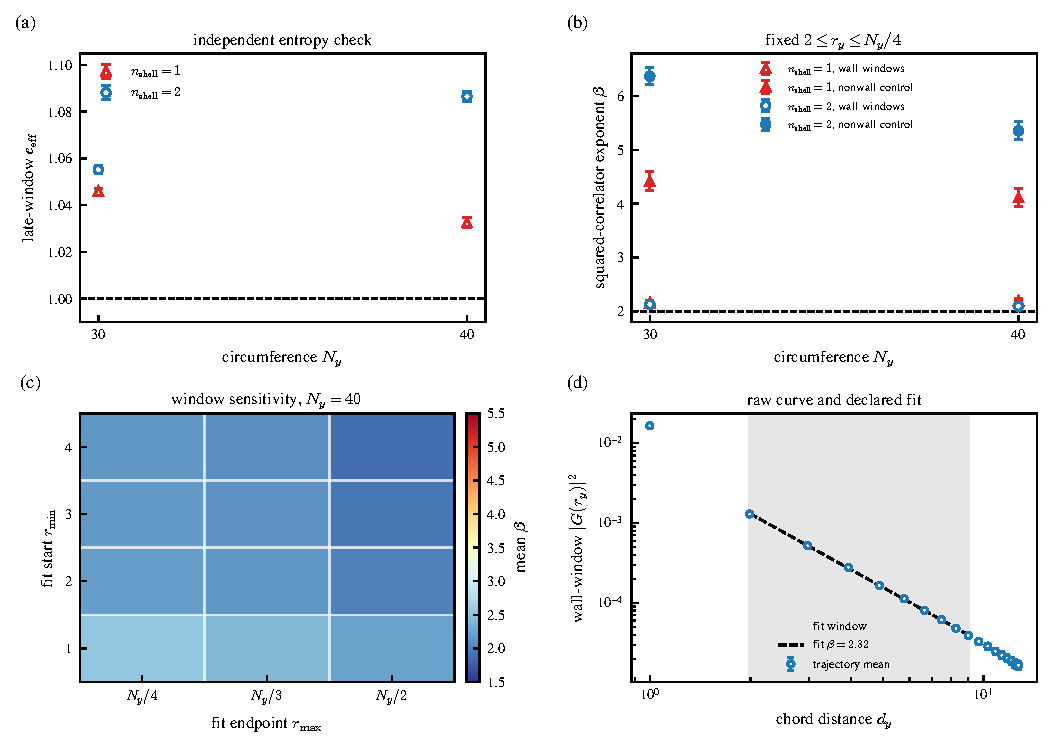
\includegraphics[width=0.98\linewidth]{result_18_small_system_state_crosscheck.pdf}
\caption{\label{fig:small-state-crosscheck}Independent pure-state cross-check.
(a) Late-window effective central charge at two shell depths; empirical points are not
connected and the dashed line is $c=1$.  (b) Squared-correlator exponents for the two wall
windows and a matched nonwall control on the fixed $2\leq r_y\leq N_y/4$ interval.
(c) Mean wall exponent as the lower and upper fit endpoints are varied; each rectangular
cell is one explicitly labeled endpoint pair.  (d) The $N_y=40$, $n_{\rm shell}=1$
trajectory-mean wall curve.  Points are unconnected, the gray region is the declared fit
window, and the dashed line is the fit.  Error bars in (a) are regression standard errors;
those in (b) and (d) are trajectory standard errors and can be smaller than the markers.
All inputs are cycle-50, $N_x=16$, $S=10$ perfect-correction covariances at
$N_y=30,40$ and $n_{\rm shell}=1,2$; Eqs.~\eqref{eq:atlas-entropy},
\eqref{eq:entropy-target}, and \eqref{eq:atlas-correlator-target} define the reductions.
Only two sizes are present, and panel (c) exposes rather than hides fit-window sensitivity.}
\end{figure*}

\subsection{Result 19: feedback reshapes the finite particle--Choi transfer mode}

The mass-sweep Colab folder contains more than the scalar gaps in Result 8.  Its executed
mode analysis maps each saved reduced-basis eigenvector back to physical unit cells.  At
$N_y=40$ and $\alpha_{\rm in}=1$, perfect correction raises the mean probability within
one column of either reduced-slab edge from $0.45187$ to $0.87933$ and lowers the mean edge
distance from $1.9944$ to $0.5745$ cells.  The site participation ratio simultaneously
falls from $156.24(728)$ to $56.72(278)$.  Along the perfect-correction branch the edge
weight decreases to $0.65428$ at $\alpha=1.5$ and $0.46673$ at $1.9$, while the mean edge
distance grows to $1.2694$ and $1.9432$.  The common-scale unit-cell maps in
Fig.~\ref{fig:transfer-modes}(c,d) show the same feedback-induced localization directly.

The terminology matters.  The legacy arrays call these ``finite Lyapunov modes,'' but
they are eigenmodes of the conditioned particle--Choi transfer construction in a reduced
topological slab basis.  They are not the covariance-tangent Oseledec modes used in
Result 2.  This classification is why the result strengthens the spatial interpretation
of the S2 transfer precursor without being promoted into a thermodynamic tangent claim.

\evidence{canonical GPU $S=10$ finite particle--Choi transfer eigenvectors; 7,151 parsed
finite-mode rows with no parse failures.}
\limittext{The basis is a conditioned reduced Choi slab, and finite-sector loss near the
transition is censoring.  The maps do not establish a physical tangent eigenmode or a
new bulk topological invariant.}

\begin{figure*}[t]
\centering
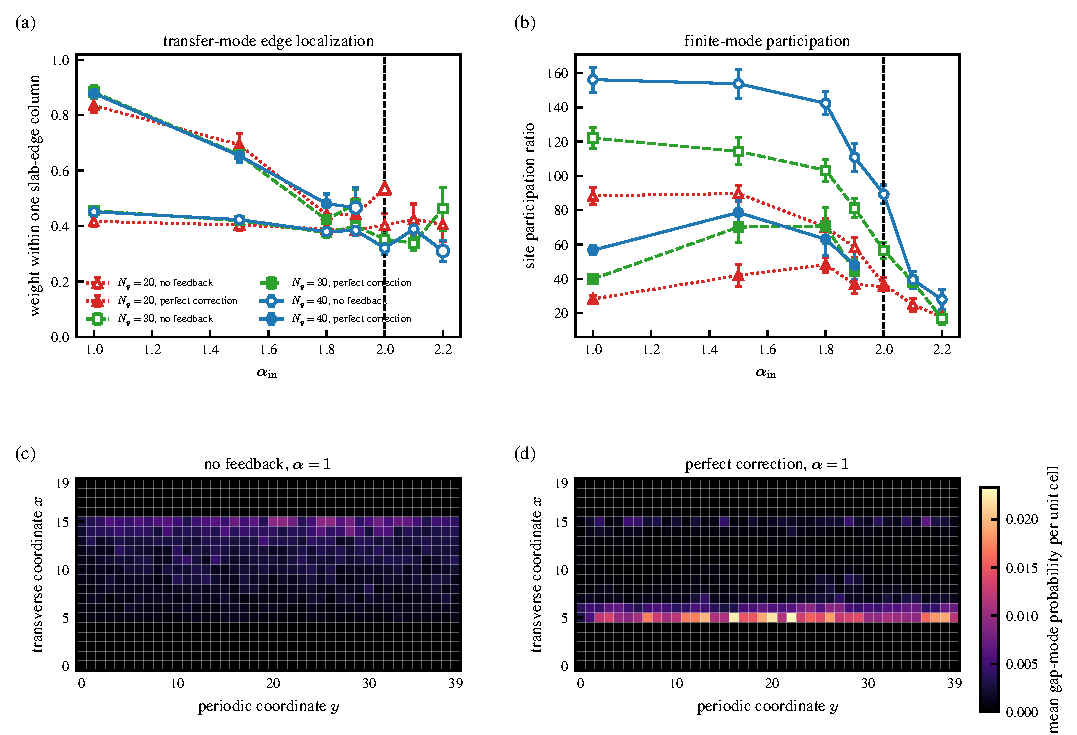
\includegraphics[width=0.98\linewidth]{result_19_transfer_mode_localization.pdf}
\caption{\label{fig:transfer-modes}Finite particle--Choi transfer-mode structure.
(a) Mean probability within one column of either reduced-slab edge and (b) site
participation ratio versus $\alpha_{\rm in}$.  Filled markers denote perfect correction;
open markers denote no feedback.  Bars are trajectory standard errors and can be smaller
than the markers; open overplots at censored points denote fewer than ten finite samples.
(c,d) Ten-trajectory mean gap-mode probability per physical unit cell at $N_y=40$ and
$\alpha=1$, plotted with one common color scale.  Thin white lines mark every unit-cell
boundary exactly; the horizontal coordinate is periodic $y$ and the vertical coordinate
is transverse $x$.  All arms use $N_x=20$, $N_y=20,30,40$, $S=10$,
$C_{\rm cyc}=2N_y$, $n_{\rm shell}=1$, and \texttt{dw\_truncation=True}; filled and
open series distinguish perfect correction and no feedback.  The saved reduced slab is
$x=5,\ldots,15$ (11 columns).  Equations~\eqref{eq:atlas-particle-choi},
\eqref{eq:atlas-particle-choi-exponents}, and \eqref{eq:atlas-transfer-mode-stats} define
the reduced-basis mode and its statistics.  These are conditioned particle--Choi modes;
censored finite sectors are not
infinite gaps, and the maps are not covariance-tangent Oseledec vectors.}
\end{figure*}

\subsection{Result 20: correct feedback was run on the untruncated overlapping interface}

The Colab charge-sharpening archive contains a completed construction that was missed in
the earlier W1 inventory.  Every untruncated run keeps \texttt{DW=True}, fixes the outer
controller at $\alpha_{\rm out}=30$, and sets \texttt{dw\_truncation=False}; the inner
parameter is swept through $\alpha_{\rm in}=1,1.5,1.8,1.9,2,2.1,2.2,2.5,3$.  Thus the
two spatial interfaces remain present while the controller projectors are allowed to
overlap them.  This is not a homogeneous \texttt{DW=False} control.  The completed
perfect-correction arm has $N_x=16$, $N_y=16,24,32$, ten trajectories per parameter
point, and $T=2N_y$: 27 configurations and 270 trajectories in total.

Mathematically, both constructions retain the same piecewise controller,
\begin{equation}
 \alpha(x)=
 \begin{cases}
  \alpha_{\rm in}, & x\in\mathcal I_{\rm top},\\
  \alpha_{\rm out}=30, & x\in\mathcal I_{\rm triv},
 \end{cases}
 \label{eq:overlap-alpha-profile}
\end{equation}
and differ only in whether controller support is terminated at the interfaces.  To avoid
mistaking the larger full-layer support for a physical enhancement, the construction
comparison uses
\begin{equation}
 \begin{aligned}
 \overline O_\gamma&=O_\gamma/N_{\rm mode}^\gamma,\\
 R_O(\alpha,N_y)&=\overline O_{\rm untruncated}/
                         \overline O_{\rm terminated},\\
 O&\in\{S_{\rm tot},\Tr[C(\mathbf{1}-C)]\}.
 \end{aligned}
 \label{eq:overlap-density-ratio}
\end{equation}

At $N_y=32$, the untruncated interface has final entropy $0.10488$, $0.26286$, and
$6.06\times10^{-5}$ at $\alpha_{\rm in}=1,1.5,1.9$, respectively, and is at the numerical
purity floor by $\alpha_{\rm in}=2$.  Its corresponding intrinsic charge variances are
$0.03279$, $0.07807$, and $4.98\times10^{-6}$.  The matched support-terminated values at
the first three parameters are entropy $0.18509$, $0.45161$, and $0.06416$, and charge
variance $0.04626$, $0.13334$, and $0.02241$.  Figure~\ref{fig:untruncated-interface}
therefore shows both the common crossover near $\alpha=2$ and the generally faster
subcritical purification of the overlapping construction.  Because the active supports
differ, panels (c,d) also report ratios per measured mode rather than comparing raw totals
alone.

\evidence{canonical CPU perfect-correction interface comparison; no post-selection arm is
used.}
\limittext{The campaign saves purification and charge-sharpening observables on the full
top layer, but not Chern profiles, log-chord entropy, tangent localization, fitted
interface leakage, or opposite-wall overlap.  It is a strong W1 construction precursor,
not the preregistered W1 equivalence gate.}

\begin{figure*}[t]
\centering
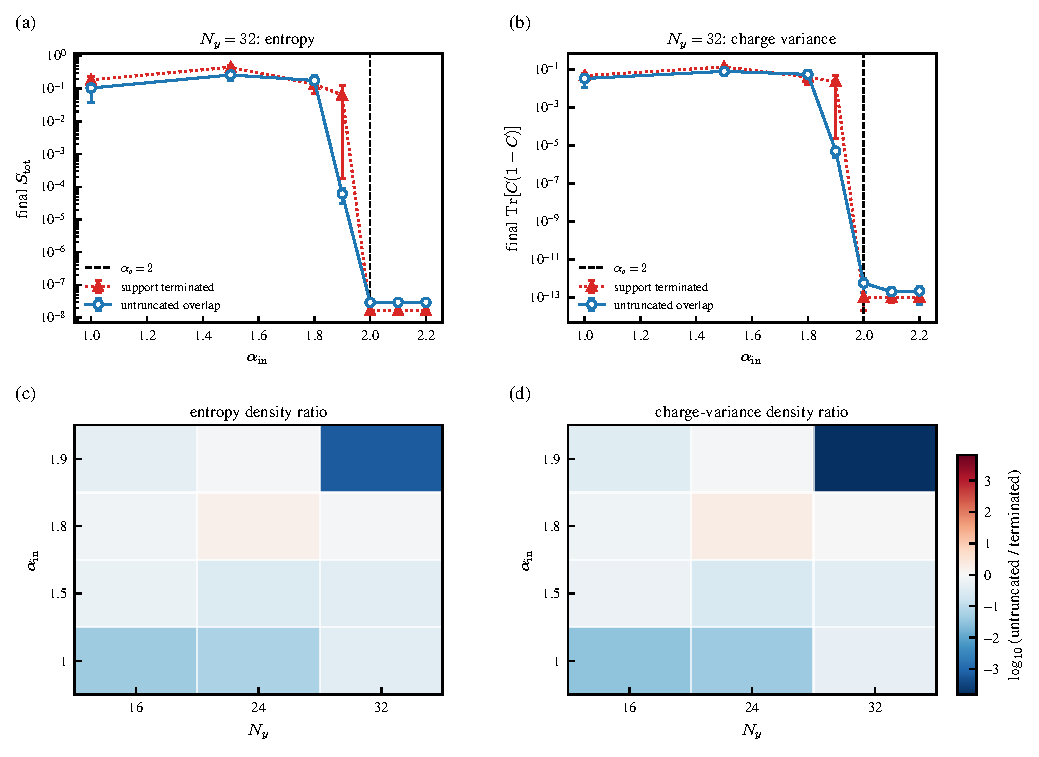
\includegraphics[width=0.98\linewidth]{result_20_untruncated_interface.pdf}
\caption{\label{fig:untruncated-interface}Perfect-correction comparison of the
support-terminated and untruncated overlapping interfaces.  (a,b) Final entropy and
intrinsic charge variance at $N_y=32$; bars are trajectory standard errors and are often
smaller than the markers.  Lines only guide the eye between the discrete simulated
$\alpha_{\rm in}$ values, the black dashed line marks $\alpha_c=2$, and values at the
right edge reach the numerical floor.  (c,d) Base-ten logarithm of the untruncated to
support-terminated ratio for entropy and charge variance per measured mode over the
subcritical sweep.  White grid lines mark individual $(\alpha_{\rm in},N_y)$
configurations exactly, and both heat maps share one color scale.  Both constructions keep
\texttt{DW=True}, use perfect correction for $2N_y$ cycles and $S=10$, and differ only
in \texttt{dw\_truncation}; Eqs.~\eqref{eq:overlap-alpha-profile} and
\eqref{eq:overlap-density-ratio} define the comparison.  It tests purification of an
overlapping interface, not topological equivalence of the two constructions.}
\end{figure*}

\subsection{Result 21: critical subsystem charge fluctuations resolve the current sector}

Figure~\ref{fig:subsystem-charge-fluctuations} presents the raw interval fit,
trajectory-resolved coefficients, matched entropy comparison, and coefficient
distributions.
The raw covariance snapshots underlying Result~18 also determine an observable that had
not been reduced in the archived characterization notebooks: the quantum fluctuation of
charge in a full-$x$ periodic interval.  For a conditioned number-conserving Gaussian
trajectory with $C=(G+\mathbf{1})/2$ and interval $A$,
\begin{equation}
 F_{A,\xi}^{\rm q}=\operatorname{Var}_{\xi}(Q_A)
 =\Tr[C_{A,\xi}(\mathbf{1}_A-C_{A,\xi})].
 \label{eq:legacy-charge-variance}
\end{equation}
This is evaluated separately for every trajectory and averaged over all periodic origins
only within that trajectory.  The calculation does not use the classical variance of the
trajectory means, and it is distinct from the full-system intrinsic variance used to
diagnose max-mix purification.

The origin average can be evaluated directly from covariance blocks.  With $d=2N_x$,
$\overline n=N_y^{-1}\Tr C$, and
$K_r=N_y^{-1}\sum_y\lVert C_{y,y+r}\rVert_F^2$,
\begin{equation}
 \overline F_{\xi}^{\rm q}(A_y)=A_y(\overline n-K_0)
 -\sum_{r=1}^{A_y-1}(A_y-r)(K_r+K_{-r}).
 \label{eq:legacy-charge-origin-average}
\end{equation}
The notebook checks Eq.~\eqref{eq:legacy-charge-origin-average} against explicit restricted
submatrices at three interval lengths in every configuration.  For a two-wall charged CFT,
\begin{equation}
 \begin{aligned}
 \overline F^{\rm q}(A_y)&=\frac{k}{\pi^2}
 \log\!\left[\frac{N_y}{\pi}\sin\!\left(\frac{\pi A_y}{N_y}\right)\right]
 +b+\cdots,\\
 k_{\rm eff}&=\pi^2m_F .
 \end{aligned}
 \label{eq:legacy-charge-level-fit}
\end{equation}

Fitting $8\leq A_y\leq N_y/2$ at cycle 50 gives
\begin{equation}
\begin{array}{c|cc}
 & n_{\rm shell}=1 & n_{\rm shell}=2\\ \hline
N_y=30 & k_{\rm eff}=1.0409(166) & 1.0468(106)\\
N_y=40 & k_{\rm eff}=1.0328(346) & 1.0853(449),
\end{array}
\label{eq:legacy-charge-level-values}
\end{equation}
where parentheses are trajectory standard errors from ten independently fitted records.
The ensemble-mean curves have $R^2>0.99996$.  These levels track the matched entropy
values $c_{\rm eff}=1.0458,1.0551,1.0324,1.0865$ in the same order.  Thus the saved
states contain a direct, near-level-one charge-sector signal rather than only an entropy
coefficient compatible with $c=1$.

\evidence{canonical GPU perfect-correction raw covariance snapshots; $N_x=16$,
$N_y=30,40$, $n_{\rm shell}=1,2$, ten trajectories, cycle 50; no partial post-selection.}
\limittext{The charge and entropy estimates use the same four trajectory ensembles, so
their agreement is a matched-observable test rather than an independent replication.
Only two circumferences and ten trajectories per configuration are available; there is no
thermodynamic extrapolation, one-wall charge decomposition, higher-cumulant analysis, or
independent chirality test in this result.}

\begin{figure*}[t]
\centering
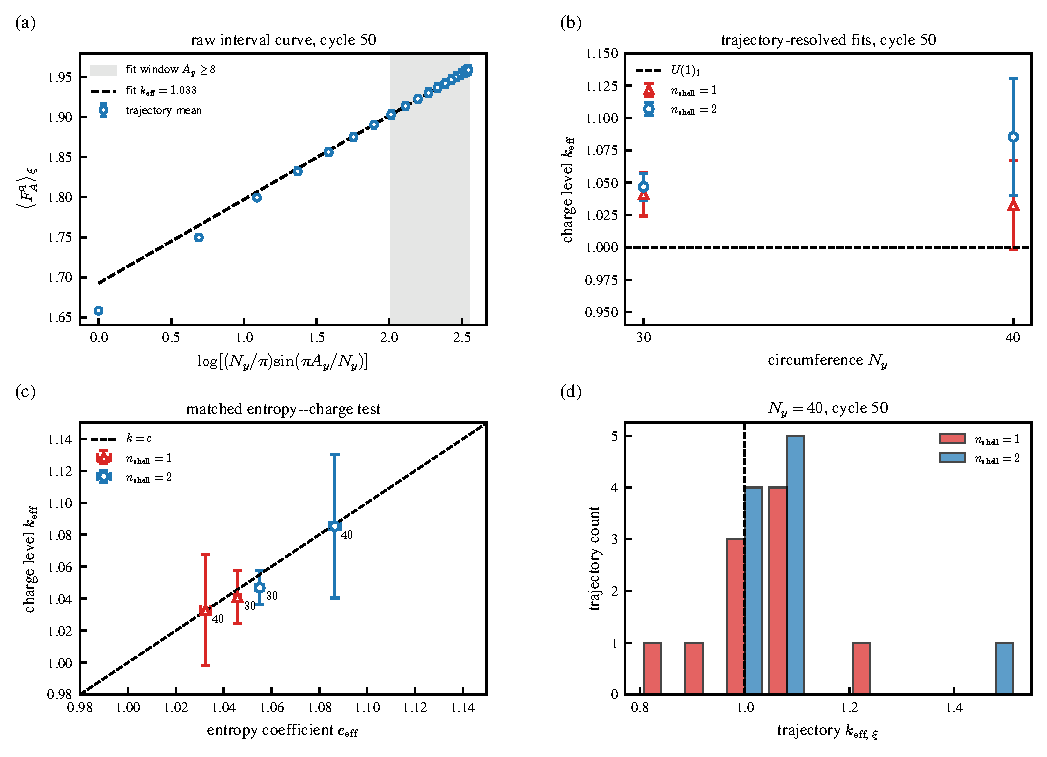
\includegraphics[width=0.98\linewidth]{result_21_subsystem_charge_fluctuations.pdf}
\caption{\label{fig:subsystem-charge-fluctuations}Critical subsystem charge fluctuations
from canonical perfect-correction covariance snapshots.  Every panel uses cycle 50.
(a) Mean full-$x$ interval variance for $N_y=40$, $n_{\rm shell}=1$; points are not
connected, the gray region is the declared $A_y\geq8$ fit window, and the dashed fitted
line is extended across the full measured range.  Bars are trajectory standard errors and
are mostly smaller than the markers.  (b) Trajectory-resolved $k_{\rm eff}$ versus size;
bars are standard errors over ten trajectory fit coefficients.  (c) Matched charge and
entropy coefficients from the same ensembles; horizontal bars are regression errors over
entropy fit points and vertical bars are trajectory standard errors.  Numerals label
$N_y$.  (d) Solid, black-outlined histograms of the ten $N_y=40$ trajectory coefficients;
the dashed references in all applicable panels mark the level-one or $k=c$ target.
Equations~\eqref{eq:atlas-charge-cumulants}--\eqref{eq:legacy-charge-level-fit} define the
cycle-50, $N_x=16$, $S=10$ reductions for $N_y=30,40$ and
$n_{\rm shell}=1,2$.  Origins are averaged inside each record before fitting; the
charge/entropy match uses the same ensembles and is not an independent replication.}
\end{figure*}

\subsection{Result 22: a three-by-three OW window preserves the target-band overlap obstruction}

Figure~\ref{fig:windowed-chern-form-factor} displays the retained norm, localization
scales, overlap zeros, and the distinction between overlap winding and compact-spinor
topology.
The circuit measures compact overcomplete-Wannier (OW) modes, so the finite support must
be checked directly against the target Chern band rather than inferred from a single
localization length.  For trial spinor $|\tau\rangle$, band form factor
$f(\mathbf{k})=\langle u_-(\mathbf{k})|\tau\rangle$, and real-space mask $g_n$, the
windowed mode has the twisted-convolution overlap
\begin{equation}
 f_n^{\rm eff}(\mathbf{k}')=\frac{1}{N}\sum_{\mathbf{k}}
 \widetilde g_n(\mathbf{k}'-\mathbf{k})f(\mathbf{k})
 \langle u_-(\mathbf{k}')|u_-(\mathbf{k})\rangle .
 \label{eq:legacy-windowed-form-factor}
\end{equation}
Its zero and local phase winding test whether the finite measurement mode still encounters
the target-band obstruction.  This diagnostic must be distinguished from the Chern number
of the compact-support spinor
\begin{equation}
 |\psi_n(\mathbf{k})\rangle=
 \sum_{\mathbf{r}\in\operatorname{supp}(g_n)}e^{-i\mathbf{k}\cdot\mathbf{r}}
 C_{\mathbf r}|\tau\rangle .
 \label{eq:legacy-windowed-spinor}
\end{equation}
When $|\psi_n(\mathbf{k})\rangle$ is smooth, periodic, and nowhere zero, it is a global
section and therefore has $C_{\psi_n}=0$; its topology is not the overlap winding.

For a normalized unwindowed OW mode centered at $\boldsymbol R$, the RMS spread, its
topological lower bound, and the asymptotic tail length are distinct quantities:
\begin{align}
 \xi_{\rm rms}^2
 &=\frac{\sum_{\boldsymbol r}|\boldsymbol r-\boldsymbol R|^2
 \|\chi_{\boldsymbol R}(\boldsymbol r)\|^2}
 {\sum_{\boldsymbol r}\|\chi_{\boldsymbol R}(\boldsymbol r)\|^2},\nonumber\\
 \xi_{\rm rms}&\geq\xi_{\rm top},\nonumber\\
 \xi_{\rm top}&=\sqrt{2|C|}\,\ell,
 \qquad 2\pi\ell^2=A_{\rm uc}.
 \label{eq:ow-localization-scales}
\end{align}
The inequality is the coherent-state spread bound of
Li, Dong, Ledwith, and Khalaf~\cite{LiDongLedwithKhalaf2024}.  Independently,
\begin{equation}
 \|\chi_{\boldsymbol 0}(\boldsymbol r)\|
 \sim e^{-|\boldsymbol r|/\xi_{\rm exp}}
 \quad (|\boldsymbol r|\to\infty),
 \label{eq:ow-exponential-length}
\end{equation}
up to algebraic prefactors, defines the exponential tail length.  Thus
$\xi_{\rm top}$ is a lower bound on the unwindowed RMS spread, not a radius that certifies
a hard truncation, and $\xi_{\rm exp}$ controls the far tail rather than the second
moment.  For the documented uniform $\alpha=1$ two-band projector and $X$ trial spinor,
$A_{\rm uc}=a^2$, $|C|=1$, and the three scales are
$\xi_{\rm top}=0.56419a$, $\xi_{\rm rms}=0.67352a$, and
$\xi_{\rm exp}=1.44270a$.  The measured RMS spread is therefore about $19.4\%$ above,
rather than at, the rigorous lower bound.  Direct Fourier reconstruction gives
\begin{equation}
\begin{array}{c|ccc}
n_{\rm shell} & \text{retained norm} & k_x^{(0)}/\pi & \nu_n\\ \hline
0 & 0.620624 & 0.209346 & -1\\
1 & 0.992155 & 0.492186 & -1\\
2 & 0.999137 & 0.492488 & -1
\end{array}
\label{eq:legacy-windowed-values}
\end{equation}
compared with the unwindowed zero at $k_x/\pi=1/2$ on $k_y=0$.  Thus the practical
$n_{\rm shell}=1$ three-by-three mask removes less than one percent of the OW norm and
only weakly displaces the obstruction zero.  A stable Fukui--Hatsugai--Suzuki evaluation
gives $C_{\psi_n}=0$ for $n_{\rm shell}\leq2$, as required.  Apparent nonzero values for
larger masks on a coarse grid are not used: the compact-spinor minimum norm is already
$2.05\times10^{-3}$ at $n_{\rm shell}=4$ and $3.36\times10^{-5}$ at
$n_{\rm shell}=8$, so that calculation does not resolve the near-singular limit.

\evidence{deterministic reconstruction of the uniform-$\alpha=1$ form-factor model;
projector Fourier grid, real-space norm, continuum overlap zeros, local winding, and the
stable compact-spinor FHS check are all recomputed in the sole atlas notebook.}
\limittext{This is a controller-design check for one model, trial spinor, gauge, and mask
family.  It contains no domain wall, disorder, conditioned trajectory, or dynamical
observable, and it does not establish the B1 static-frame prediction criterion.}

\begin{figure*}[t]
\centering
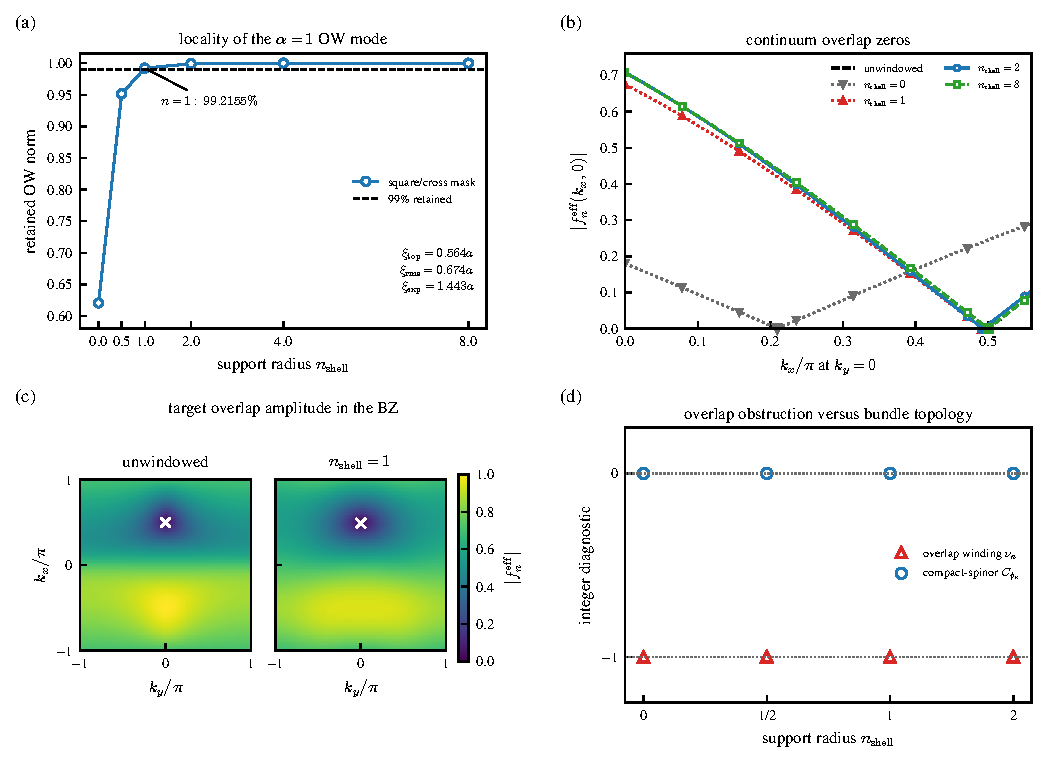
\includegraphics[width=0.98\linewidth]{result_22_windowed_chern_form_factor.pdf}
\caption{\label{fig:windowed-chern-form-factor}Finite-shell OW form-factor audit for the
uniform $\alpha=1$ projector and $X$ trial spinor.  (a) Fraction of projected-mode norm
retained by each square or cross mask, together with the topological, RMS, and exponential
localization scales defined in Eqs.~\eqref{eq:ow-localization-scales} and
\eqref{eq:ow-exponential-length}.  These are properties of the unwindowed mode, not hard
window radii.  (b) $k_y=0$ cuts of the target-band overlap; symbols mark the
continuum-minimized zeros, and lines show the corresponding overlap functions rather than
fits.  (c) Unwindowed and $n_{\rm shell}=1$ overlap-amplitude maps over the Brillouin zone;
white crosses mark the zeros.  (d) The target-band overlap winding remains $\nu_n=-1$
while the smooth compact-support spinor has $C_{\psi_n}=0$.  Coarse-grid FHS values at
$n_{\rm shell}=4,8$ are deliberately omitted because the spinor is too close to singular
for a stable bundle diagnostic.  The deterministic uniform-$\alpha=1$ calculation uses
Eqs.~\eqref{eq:ow-localization-scales}, \eqref{eq:legacy-windowed-form-factor},
\eqref{eq:atlas-overlap-magnitude}, and \eqref{eq:legacy-overlap-chern-index}; lines in
(b) are functions, not fits.  The result
tests one $X$ trial spinor and mask family, not a domain-wall trajectory.}
\end{figure*}

\subsection{Result 23: overlap winding follows the target Bloch-bundle phase}

Figure~\ref{fig:overlap-winding-alpha-sweep} shows the resolved overlap zeros and winding
through the topological and trivial mass values in the sweep.
The winding in Result~22 is not merely the visual circulation around a convenient dip.
Let $L\to T^2$ be the occupied-band line bundle and choose local frames related on patch
overlaps by $|u_j\rangle=e^{i\chi_{ij}}|u_i\rangle$.  For any smooth periodic trial field
$|\phi_n(\mathbf{k})\rangle$, including the unwindowed trial spinor and either finite OW
mask,
\begin{equation}
 f_{n,i}(\mathbf{k})=\langle u_i(\mathbf{k})|\phi_n(\mathbf{k})\rangle,
 \qquad f_{n,j}=e^{-i\chi_{ij}}f_{n,i}.
 \label{eq:legacy-overlap-dual-section}
\end{equation}
Thus $f_n$ is a section of the dual bundle $L^*$.  If its zeros are isolated, their local
indices may be related to $C$ directly, without taking a zero-index theorem as a black
box.  Delete counterclockwise disks $D_a$ around the zeros and set
$M=T^2\setminus\bigcup_aD_a$.  On $M$ the normalized projected trial state
\begin{equation}
 |v_n\rangle=\frac{P_-|\phi_n\rangle}{\|P_-|\phi_n\rangle\|}
 =e^{i\arg f_{n,i}}|u_i\rangle
 \label{eq:legacy-overlap-projected-frame}
\end{equation}
is a gauge-independent, single-valued occupied-band frame.  If
$A_i=-i\langle u_i|d u_i\rangle$, its connection is
$A_v=A_i+d\arg f_{n,i}$ and has curvature $F=dA_i$.  Stokes' theorem on the punctured
torus therefore gives
\begin{equation}
 \begin{aligned}
 2\pi C&=\lim_{D_a\to0}\int_MF
 =\lim_{D_a\to0}\oint_{\partial M}A_v\\
 &=-\sum_a\lim_{D_a\to0}\oint_{\gamma_a}
 \bigl(A_i+d\arg f_{n,i}\bigr)
 =-2\pi\sum_a\nu_a.
 \end{aligned}
 \label{eq:legacy-overlap-stokes-proof}
\end{equation}
Each hole occurs clockwise in $\partial M$, producing the minus sign, while the integral
of smooth $A_i$ vanishes as its disk shrinks.  Hence
\begin{equation}
 \sum_a\nu_a
 =\sum_a\frac{1}{2\pi}\oint_{\gamma_a}d\arg f_n
 =-C.
 \label{eq:legacy-overlap-chern-index}
\end{equation}
A nonzero target-band Chern number therefore forces overlap zeros even though a smooth,
nonvanishing compact spinor $|\phi_n\rangle$ defines a trivial bundle of its own.  In
particular, the $n_{\rm shell}=0$ compact spinor has Chern number zero, but its overlap
has winding $-1$ when the target band has $C=+1$.  When $C=0$, accidental
zero--antizero pairs remain possible, but their total index must vanish.

The numerical implementation first evaluates the gauge-invariant magnitude
\begin{equation}
 |f_n(\mathbf{k})|^2=
 \langle\phi_n(\mathbf{k})|P_-(\mathbf{k})|\phi_n(\mathbf{k})\rangle
 \label{eq:legacy-overlap-magnitude}
\end{equation}
on a periodic $181\times181$ grid.  It identifies all discrete local minima, refines the
lowest 32 candidates by periodic two-dimensional Nelder--Mead minimization, and merges
coincident solutions.  A refined residual below $10^{-6}$ is classified as a zero.  For
each zero, one reference spinor $|r_a\rangle$ is chosen at its center and held fixed on a
radius-$0.02$ loop, defining the smooth local frame
\begin{equation}
 \begin{aligned}
 |u_a^{\rm loc}(\mathbf{k})\rangle
 &=\frac{P_-(\mathbf{k})|r_a\rangle}
 {\|P_-(\mathbf{k})|r_a\rangle\|},\\
 \nu_a
 &=\operatorname{round}\!\left[
 \frac{1}{2\pi}\left\{\operatorname{unwrap}\arg
 f_n(\mathbf{k}(\theta))\right\}_{\theta=0}^{2\pi}\right].
 \end{aligned}
 \label{eq:legacy-overlap-loop-algorithm}
\end{equation}
The loop uses 721 angular samples.  An independent FHS surface integral supplies $C$ for
the target lower band.  A positive refined global minimum is reported as a gapped overlap,
not assigned a spurious winding around an arbitrary minimum.

For the requested sweep the result is
\begin{equation}
\begin{array}{c|c|cccc}
\alpha&C&\nu_{\rm none}&\nu_0&\nu_1&\nu_2\\ \hline
1   &+1&-1&-1&-1&-1\\
1.5 &+1&-1&-1&-1&-1\\
3   &0&0&0&0&0\\
30  &0&0&0&0&0
\end{array}
\label{eq:legacy-overlap-alpha-sweep}
\end{equation}
Here ``none'' means no real-space truncation.  The zero locations
$k_x^{(0)}/\pi$ for $(\text{none},0,1,2)$ are
$(0.500000,0.209346,0.492186,0.492488)$ at $\alpha=1$ and
$(0.333333,0.064606,0.346511,0.345054)$ at $\alpha=1.5$, with
$|k_y^{(0)}|/\pi<4\times10^{-9}$.  All eight phase-circulation calculations give one
isolated zero with $\nu=-1$.  The $n_{\rm shell}=0$ compact spinor therefore has
$C_{\psi_0}=0$ while its overlap has turn number $-1$: the two invariants are not the same.
At $\alpha=3,30$, the respective global overlap minima for
$(\text{none},0,1,2)$ are
$(0.500000,0.652414,0.525837,0.499765)$ and
$(0.694808,0.706710,0.694824,0.694800)$.  These positive gaps exclude zeros for all four
trial fields, so the total winding is zero, exactly tracking the independently computed
change from $C=1$ to $C=0$.

\evidence{deterministic global-zero search, local phase circulation, and independent
target-band FHS check for the two-band $X$-trial model.}
\limittext{The sweep tests four mass values and three square masks.  It is not a
finite-size or trajectory calculation and does not resolve the critical point
$\alpha=2$, where the target-band gap closes and $C$ is undefined.}

\begin{figure*}[t]
\centering
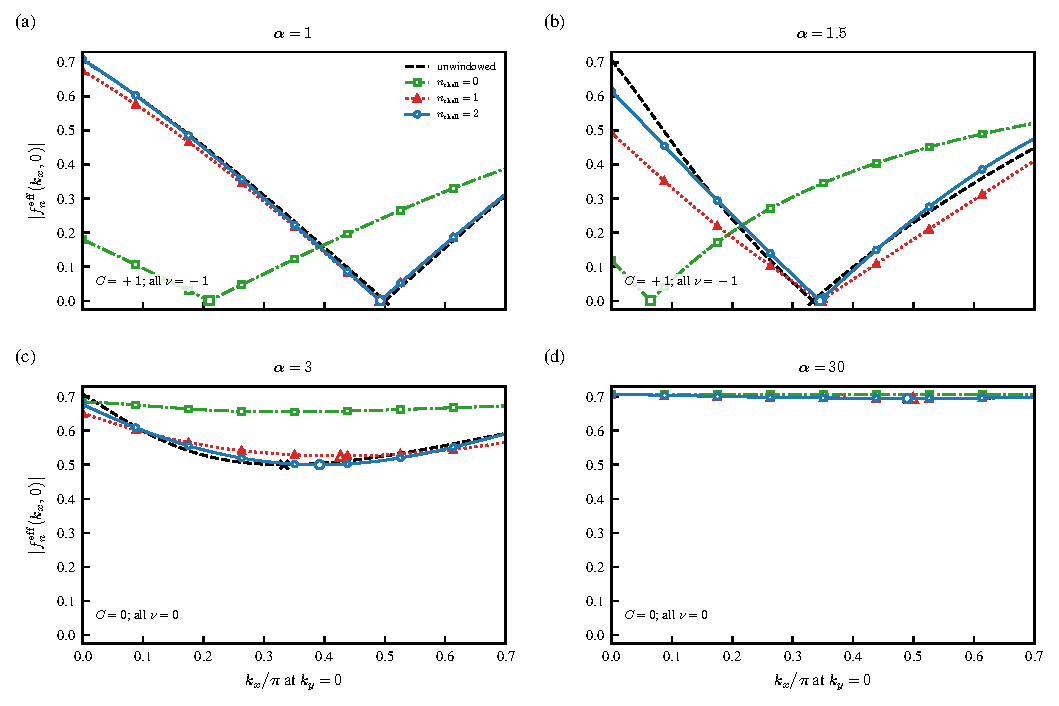
\includegraphics[width=0.98\linewidth]{result_23_overlap_winding_alpha_sweep.pdf}
\caption{\label{fig:overlap-winding-alpha-sweep}Overlap-winding sweep for the unwindowed
and $n_{\rm shell}=0,1,2$ $X$-trial modes.  (a,b) In the $C=+1$ phase at
$\alpha=1,1.5$, every overlap has one resolved zero on $k_y=0$ and total winding $-1$;
large symbols mark the refined zeros.  (c,d) In the trivial phase at $\alpha=3,30$, every
curve remains strictly positive and has total winding zero.  Lines are deterministic
$k_y=0$ overlap cuts, not fits; positive global minima are quoted in the text, and the displayed $C$
values come from an independent full-BZ FHS calculation.  The zero search, local
circulation, and bundle relation are Eqs.~\eqref{eq:legacy-overlap-magnitude}--
\eqref{eq:legacy-overlap-chern-index}; there are no sampling bars.  The four-point sweep
excludes $\alpha=2$, where the isolated-band Chern number is undefined.}
\end{figure*}

\clearpage
\section{Group V: record-discarded mean channel and continuous Lindbladian}
\label{sec:mean-channel-group}

\subsection{Result 24: stationary interface occupations and deterministic density response}
\label{sec:result24}

The autonomous trajectory-averaged channel is analytically closed at the one-body level,
so neither Born trajectories nor random schedule descendants are required.  We evaluate
the exact completely positive affine Gaussian channel and its continuous weak-success
generator at fixed physical time.  The hybrid reconstruction uses $N_x=20$.  The
eight-point static mass scan is restricted to $N_y=64$, while the
$(\alpha_{\rm in},\alpha_{\rm out})=(1,30)$ response endpoint uses $N_y=32,48,64$,
$n_{\rm shell}=1,2,\mathrm{None}$, and domain-wall-sector truncation both on and off.  The
canonical arm keeps that truncation on.  It starts from
$C(0)=\frac12\mathbf{1}$, uses no burn-in, and observes state relaxation through $2N_y$.

Here ``untruncated controller'' means $n_{\rm shell}=\mathrm{None}$, not
\texttt{dw\_truncation=False}.  Because the unwindowed controller remains exactly
translation invariant in $y$, its gain and loss frame operators are inverse-Fourier
transformed on the physical-$y$ index into independent $2N_x\times2N_x$ matrices
$V_\pm(k_y)$.  Before this block reduction, these positive frame operators are
\begin{equation}
 V_\pm=\sum_{\boldsymbol r,\nu=A,B}
 |\chi_{\boldsymbol r,\nu,\pm}\rangle
 \langle\chi_{\boldsymbol r,\nu,\pm}|,
 \label{eq:mean-frame-operators}
\end{equation}
with the normalized modes of Eq.~\eqref{eq:ow-modes}.  The scalar
$n_a\in[0,1]$ is the prescribed ancilla filling, equivalently the gain weight; every
displayed Result-24 arm uses $n_a=1/2$.  For every momentum, the deterministic covariance satisfies
\begin{align}
 \dot C(k_y)&=n_aV_-(k_y)-\frac12\{D(k_y),C(k_y)\},
 \label{eq:mean-generator}\\
 D(k_y)&=n_aV_-(k_y)+(1-n_a)V_+(k_y),
 \label{eq:mean-damping}\\
 &D(k_y)C_{\rm ss}(k_y)\nonumber\\
 &\quad+C_{\rm ss}(k_y)D(k_y)=2n_aV_-(k_y).
 \label{eq:stationary-lyapunov}
\end{align}
Equation~\eqref{eq:stationary-lyapunov} is solved separately in each momentum block and
each $C_{\rm ss}(k_y)$ is then diagonalized.  No sliding window, convolution, or average
over $y$ is used to create Fig.~\ref{fig:continuous-lindblad-interface}(a): its
$k_y$ resolution is an exact symmetry decomposition.  Both
\texttt{dw\_truncation=True} and false curves in that panel are $k_y$ resolved because
both use $n_{\rm shell}=\mathrm{None}$; finite-shell products are deliberately not
assigned a momentum spectrum.

At each wall $x_w$, the mode weight is the sum over both orbitals and the three columns
$x_w-1,x_w,x_w+1$.  Modes with weight at least $0.25$ are eligible, and the selected mode
minimizes
\begin{equation}
 \mathcal J_a(k_y)=|\nu_a(k_y)-\tfrac12|
 +0.02\,[1-w_a(k_y)].
 \label{eq:mean-branch-selection}
\end{equation}
If no mode reaches the threshold at a momentum, the maximum-weight mode is used as an
explicit fallback.  A straight line is fit only for
$|k_y|\leq\max(2.5\,2\pi/N_y,0.22)$.  At $N_y=64$ the two wall-selected branches cross
half occupation with fitted slopes $\pm0.949605$.  This is a
stationary mixed-state occupation-band statement, not physical-time or twist spectral
flow and not preparation of a pure chiral critical state.  Finite-shell products remain
strictly real-space or integrated.

For the dynamical probe, exact local $\pm\epsilon$ density-phase unitaries with
$\epsilon=10^{-3}$ are central-differenced about $C_{\rm ss}$.  If
$\delta n_w(y,t)$ is the response summed over the same wall window, its positive-lobe
center and fitted velocity are
\begin{align}
 y_{+,w}(t)&=\frac{\sum_y\widetilde y\,[\delta n_w(y,t)]_+}
 {\sum_y[\delta n_w(y,t)]_+},\nonumber\\
 v_{+,w}&=\frac{\dd y_{+,w}}{\dd t},\qquad
 \mathcal D_w=
 \left\langle\frac{\sum_y\widetilde y\,\delta n_w(y,t)}
 {\sum_y|\delta n_w(y,t)|}\right\rangle_{t\in\mathcal W_{\rm fit}},
 \label{eq:mean-response-velocity}
\end{align}
where $\widetilde y$ is the signed periodic displacement from the source and
$[q]_+=\max(q,0)$; $\mathcal D_w$ is the panel's signed directionality averaged over
the same active fit-time window.  The signed response has
positive-lobe velocities $(+0.077455,-0.077455)$ on the two canonical walls at $N_y=64$,
with $R^2>0.9975$ and stable signs at all three circumferences.  Turning off
domain-wall-sector truncation preserves the signs while reducing the magnitudes to
$(+0.038030,-0.038030)$.  Uniform topological and trivial controls return the numerical
null.  This is wall-resolved directional density response, not quantized conductance;
gain/loss dynamics do not provide a conserved-charge continuity equation.

For $p=1,1/2,1/4,1/8,1/16$, exact gain/loss semigroups are composed with Strang splitting
and the response is compared with the continuous solution at fixed time $N_y/2$.  The
fitted response-convergence order is $2.0008$.  Neither a covariance matrix nor a
covariance response history is archived.

\evidence{deterministic complex128 CPU reconstruction of the exact affine mean channel
and continuous gain/loss generator, with compact shell-validated outputs.}
\limittext{The calculation is an averaged channel-level statement.  It does not replace
conditioned-trajectory observables, and only $n_{\rm shell}=\mathrm{None}$ supports a
$k_y$-resolved spectral claim.}

\begin{figure*}[t]
\centering
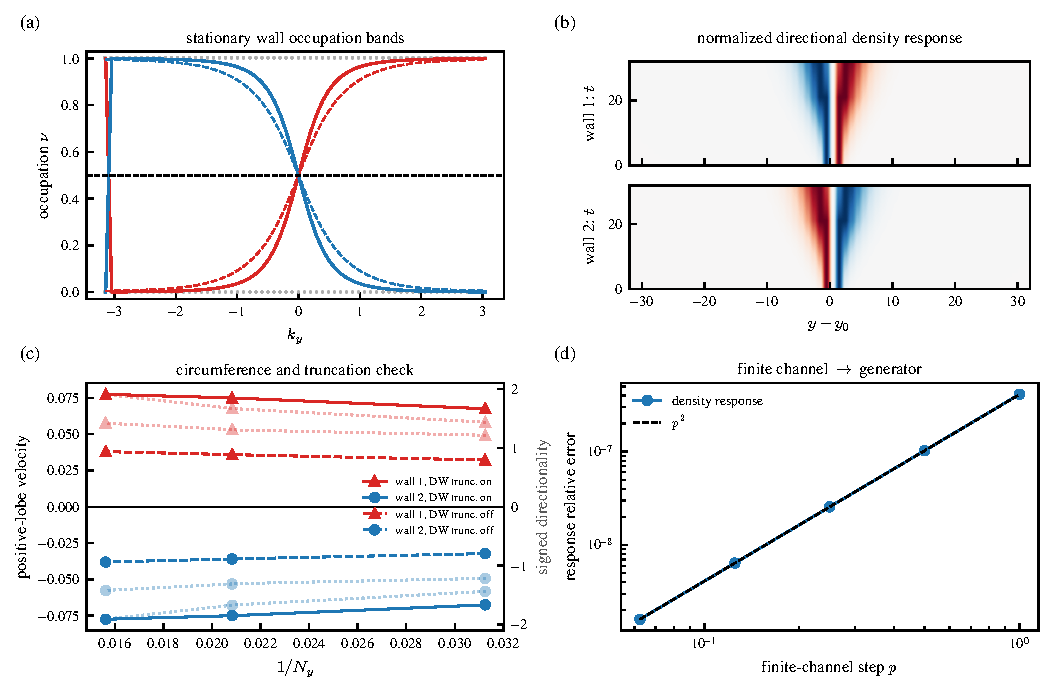
\includegraphics[width=0.98\linewidth]{result_24_continuous_lindblad_interface.pdf}
\caption{\label{fig:continuous-lindblad-interface}Exact averaged-channel interface
diagnostics.  (a) The $k_y$-resolved occupation spectrum and wall-selected branches for
$N_x=20$, $N_y=64$, $n_{\rm shell}=\mathrm{None}$, $n_a=1/2$, and
$(\alpha_{\rm in},\alpha_{\rm out})=(1,30)$.  Exact $y$-translation symmetry gives
independent $2N_x\times2N_x$ $V_\pm(k_y)$ blocks from Eq.~\eqref{eq:mean-frame-operators};
Eqs.~\eqref{eq:stationary-lyapunov} and \eqref{eq:atlas-lyapunov-solution} are solved and
the resulting $C_{\rm ss}(k_y)$ is diagonalized at each $k_y$.  There is no sliding
average over $y$.  Solid and dashed
curves denote \texttt{dw\_truncation=True} and false, respectively; both are momentum
resolved because both are unwindowed.  The colored branches use the three-column wall
weight, $25\%$ eligibility gate, half-occupation cost, fallback, and near-zero-momentum fit
of Eq.~\eqref{eq:mean-branch-selection}, using
$|k_y|\leq\max(2.5\,2\pi/N_y,0.22)$.  (b) Signed central-difference density responses
to local $\pm10^{-3}$ phase kicks at the two walls, with each nonzero time slice normalized
by its own maximum absolute amplitude only for display.  The underlying response used in
fits is not slice-normalized; this panel is the $N_y=64$, unwindowed,
\texttt{dw\_truncation=True} arm through $t=N_y/2$.  (c) Positive-lobe velocities from
Eq.~\eqref{eq:mean-response-velocity} and signed directionality versus $1/N_y$ for
$N_y=32,48,64$, $n_{\rm shell}=\mathrm{None}$, and both domain-wall truncation settings;
each velocity fit uses $2\leq t\leq0.375N_y$.  (d) Relative response errors at fixed
$t=N_y/2$ for the $N_y=64$ exact gain/loss affine channels at
$p=1,1/2,1/4,1/8,1/16$; their slope tests second-order convergence to the continuous
generator.  All panels are deterministic and
therefore have no trajectory error bars.  The occupation slope is not a group velocity,
and the response velocity is not a quantized conductance.}
\end{figure*}

\clearpage
\section{Numerical ledger and source map}

Tables~\ref{tab:ledger-a} and \ref{tab:ledger-b} are the compact lookup tables for future
work.  Source entries are
deliberately given as useful repository subfolders rather than unwieldy full file paths;
the exact files are recorded in \subfolder{figure_manifest.json}.

\begin{table*}[!t]
\centering
\caption{\label{tab:ledger-a}Summary of archived numerical findings, Results 1--12.}
\scriptsize
\setlength{\tabcolsep}{2.5pt}
\renewcommand{\arraystretch}{1.04}
\begin{tabularx}{\textwidth}{p{0.035\textwidth}p{0.19\textwidth}Xp{0.25\textwidth}}
\toprule
No. & result & strongest quantitative content & reusable source subfolder \\
\midrule
1 & Exact wall benchmark & $c=1.000092$; correlator exponent $2.074$; modular velocities
$(-2.930,+4.536)$; unit signed twist flows; $N_x=20$ accepted. &
\subfolder{experiment_review/b0_exact_domain_wall/} \\
2 & Slow tangent sector & CPU wall/uniform contrast $0.101$--$0.112$ versus $0.894$--$0.896$;
GPU $0.0197$--$0.0270$ versus $0.722$--$0.768$; wall weight $0.933$--$0.996$. &
\subfolder{topological_frustration_diagnostics/}; \subfolder{colab_lyapunov/} \\
3 & Wall purification residual & At $2N_y$, $S=0.244$--$0.331$ and $V_Q=0.0665$--$0.0973$;
$94.25\%$ of a smaller-run residual lies on the wall columns. &
\subfolder{colab_charge_fluctuations/}; \subfolder{colab_small_system_testing/} \\
4 & Log-chord entropy & Common-depth $c_{\rm eff}=1.0672$, $1.0528$, $1.0476$ for
$N_y=30,40,50$; separate time-scaled series reaches $1.04098$ at $N_y=100$;
all controlled fits have $R^2>0.99997$. &
\subfolder{colab_large_entanglement_scaling_N20/} \\
5 & Tripartite information & Exact $c_{\rm TMI}=1.001806$ per wall and $1.002697$ over
both walls, with full/wall slope ratio $2.00178$; the stochastic pilot preserves counting
but gives biased $c_{\rm TMI}=1.49$--$1.58$. &
\subfolder{exact_DW_benchmark_notes/}; \subfolder{sample_average_testing/} \\
6 & Uniform Chern response & Final means $0.999995$, $0.999687$, $0.999927$ at
$N_y=30,40,50$; global minimum $0.992548$. &
\subfolder{colab_lyapunov/} \\
7 & Feedback activity & Wall activity enhanced by $4.47$--$4.84$; independently measured
tangent gap suppressed by $7.94$--$8.83$; two sharp interface peaks. &
\subfolder{topological_frustration_diagnostics/} \\
8 & $\alpha$ transition & Transfer and max-mix entropy/variance diagnostics all change
sharply near the exact $\alpha_c=2$; finite-sector loss is explicitly censored. &
\subfolder{colab_no_feedback_alpha_sweep_transfer/}; \subfolder{colab_charge_fluctuations/} \\
9 & Modular handedness & Exact modular velocities $(-2.930,+4.536)$; stochastic packet
displacements have the orientation-dependent endpoint sign pattern at two shell choices. &
\subfolder{experiment_review/b0_exact_domain_wall/}; \subfolder{colab_small_system_testing/} \\
10 & Record uncertainty & $\widehat H_{\rm chain}/N_y=2.989$--$2.995$; wall-neighborhood
uncertainty $0.1013$ versus $0.0101$ nats per event outside. &
\subfolder{colab_charge_fluctuations/} \\
11 & Flattened spectrum & Translation-resolved $X,Y,Z$ parents show two in-gap branches;
the $X,Y$ zero-energy crossings are especially clean. &
\subfolder{exact_DW_benchmark_notes/}; \subfolder{notebooks/} \\
12 & Corrected flattened-parent audit & The uniform $n_{\rm shell}=1$ parent is gapped
with $\mathcal C_R=-0.999999829$ and independent $C_{\rm FHS}=-1$ on the same occupied
projector; the $\alpha=3$ control
is trivial.  In the separate wall geometry, one shell gives entropy slopes
$0.33398/0.16675$, while the correlator exponent converges from $3.2033$ to $2.0042$. &
\subfolder{notebooks/flattened_hamiltonian_analysis/} \\
\bottomrule
\end{tabularx}
\end{table*}

\begin{table*}[p]
\centering
\caption{\label{tab:ledger-b}Summary of archived numerical findings, Results 13--24.}
\scriptsize
\setlength{\tabcolsep}{2.5pt}
\renewcommand{\arraystretch}{1.04}
\begin{tabularx}{\textwidth}{p{0.035\textwidth}p{0.19\textwidth}Xp{0.25\textwidth}}
\toprule
No. & result & strongest quantitative content & reusable source subfolder \\
\midrule
13 & Spatial evidence maps & Exact Chern, slow-vector, entropy-contour, and charge-variance
maps independently resolve the two-wall geometry. &
\subfolder{exact_DW_benchmark_notes/}; \subfolder{colab_lyapunov/};
\subfolder{colab_small_system_testing/}; \subfolder{colab_charge_fluctuations/} \\
14 & Modular density maps & Cycle-$50$ modular snapshots at $t_{\rm mod}=0,8,16,32$
display the spatial propagation underlying the endpoint sign reduction. &
\subfolder{colab_small_system_testing/} \\
15 & Trajectory distributions & $c_{\rm eff}$ and $\mathcal C$ are typically near one,
but low-Chern records and broad, right-skewed max-mix $V_Q$ tails remain. &
\subfolder{colab_charge_fluctuations/} \\
16 & Cleaning sensitivity & Charge-, wall-, and Chern-conditioned $c_{\rm eff}$ shifts are
not uniform across size or retained fraction; $10\%$ retains only ten records. &
\subfolder{colab_charge_fluctuations/analysis_outputs/} \\
17 & Filling-distribution narrowing & At $C=2N_y$, $\sigma_\nu^2$ falls
$0.29684\to0.16534$ (pure state) and $0.28533\to0.17023$ (max mix) from
$N_y=30\to50$, reductions of $44.3\%$ and $40.3\%$. &
\subfolder{colab_charge_fluctuations/} \\
18 & Independent state-data cross-check & $c_{\rm eff}=1.032$--$1.086$ and fixed-window
wall exponents $2.092$--$2.191$ at $n_{\rm shell}=1,2$; nonwall controls are $4.11$--$6.37$.
& \subfolder{colab_small_system_testing/};
\subfolder{colab_charge_fluctuations/analysis_outputs/correlator_scaling_diagnostics/} \\
19 & Conditioned transfer-mode localization & At $N_y=40$, $\alpha=1$, perfect correction
raises one-column edge weight $0.45187\to0.87933$ and lowers mean edge distance
$1.9944\to0.5745$ cells. &
\subfolder{colab_no_feedback_alpha_sweep_transfer/} \\
20 & Untruncated overlapping interface & With \texttt{DW=True},
$\alpha_{\rm out}=30$, and support truncation disabled, 270 perfect-correction
trajectories show a sharp purification crossover near $\alpha_{\rm in}=2$; at
$N_y=32$, $S_{\rm tot}$ falls $0.26286\to6.06\times10^{-5}$ from
$\alpha_{\rm in}=1.5\to1.9$. &
\subfolder{colab_charge_fluctuations/} \\
21 & Critical subsystem charge fluctuations & Cycle-50 trajectory fits give
$k_{\rm eff}=1.033$--$1.085$ across $N_y=30,40$ and $n_{\rm shell}=1,2$; matched entropy
coefficients are $c_{\rm eff}=1.032$--$1.086$, and every mean charge curve has
$R^2>0.99996$. &
\subfolder{colab_small_system_testing/gpu_data/pure_state_covariance_snapshots/} \\
22 & Finite-shell OW obstruction & The $n_{\rm shell}=1$ three-by-three mask retains
$99.2155\%$ of the OW norm, shifts the overlap zero only from $0.5$ to $0.4922$, and
preserves $\nu_n=-1$, while the compact spinor has $C_{\psi_n}=0$. &
\subfolder{form_factor_analysis/} \\
23 & Overlap-winding mass sweep & Unwindowed and $n_{\rm shell}=0,1,2$ modes all have
$\nu=-1$ at $\alpha=1,1.5$ where $C=+1$; at $\alpha=3,30$ all four overlaps are gapped
and have $\nu=0$ where $C=0$. &
\subfolder{form_factor_analysis/} \\
24 & Exact mean-channel interface & At $N_y=64$ the canonical untruncated arm has paired
half-occupation wall branches with slopes $\pm0.949605$; its two walls have signed
positive-lobe velocities $\pm0.077455$, while the finite-channel response converges to the
continuous generator with order $2.0008$ at fixed time. &
\subfolder{mean_channel_lindblad_cpu_campaign/};
\subfolder{experiment_review/legacy_evidence_figure_atlas/data/} \\
\bottomrule
\end{tabularx}
\end{table*}

\section{What the repository already says, and what remains open}

Taken together, the legacy archive already supports a coherent but carefully qualified
picture.  The deterministic wall has the intended $c=1$ topology and handedness.  The
adaptive ensemble has a near-unit bulk Chern response.  Introducing a wall produces a
strongly localized slow tangent sector, concentrates wrong-outcome activity there, delays
max-mix purification there, and leaves an entropy curve close to the two-wall $1/3$
coefficient.  Independent modular and probability-record observers see the same spatial
organization: oriented packet motion in the former and roughly tenfold wall-enhanced
uncertainty in the latter.  Independent mass sweeps further place the dynamical crossover
near the exact $\alpha=2$ transition.  The flattened parent sharpens the static benchmark:
its translation-resolved spectrum exposes the counter-propagating wall branches directly,
the uniform one-shell parent is independently gapped and Chern nontrivial, and the wall
shell hierarchy warns that a good entropy coefficient can precede convergence of local
correlator tails.  The independent OW form-factor reconstruction adds a
more microscopic support check: the actual three-by-three controller mode preserves the
target-band overlap zero and winding while retaining more than $99\%$ of its norm, without
misidentifying that overlap obstruction as a Chern number of the compact spinor.  The
four-point mass sweep makes the bundle relation explicit: all four tested overlaps have
$\sum_a\nu_a=-1$ on the $C=1$ side and a finite overlap gap with zero winding on the
$C=0$ side.  Spatial
heat maps show where each signal lives, and
trajectory histograms show that the near-universal behavior is typical rather than exact
record by record.  The size-normalized filling distribution also narrows with
circumference in two independent $S=100$ preparations.  The independent $N_x=16$
covariance snapshots reproduce the joint near-$c=1$/wall-correlator pattern at two shell
depths.  Their newly reduced subsystem charge fluctuations add the missing direct
current-sector precursor: $k_{\rm eff}$ is near one and quantitatively tracks the matched
entropy coefficient on all four available ensembles.  The transfer-mode maps show how
feedback reorganizes the conditioned
reduced-slab sector.  The newly recovered $\texttt{DW=True}$, untruncated
perfect-correction sweep further shows that the explicit interface survives overlapping
controller support and undergoes the same sharp purification crossover near $\alpha=2$,
although it purifies faster than the terminated slab below the transition.  This is
substantially more than a collection of isolated plots: it is
a mutually compatible evidence network spanning state topology, entanglement, conditional
stability, controller activity, purification, handedness, effective-parent spectra,
quantum charge fluctuations, and classical records.

The missing step is equally clear.  Most stochastic statements are assembled from
different campaigns rather than measured jointly on the accepted $S=100$ master
trajectories.  Consequently the archive does not yet prove the recordwise
tangent--purification identity, a causal activity--gap relation, a fully controlled
thermodynamic $c=1$ extrapolation with its charge sector, frozen-record integer twist flow,
physical Born susceptibility, or record-only CFT universality.  The atlas should therefore
be used as a benchmark and data index: it says exactly which signals are already present,
where their arrays live, how broad their trajectory distributions are, and which stronger
claims still require new experiments.  In particular, ensemble conditioning remains an
explicit sensitivity diagnostic rather than a license to discard inconvenient records.

\appendix

\section{Complete computation formalism for the atlas}
\label{app:formalism}

This appendix states every reduction used in Figs.~1--24.  Its purpose is conceptual and
reproducibility-oriented: the truth notebook remains the executable source, whereas the
equations below say precisely what that source computes.  An overbar denotes the
trajectory-first average in Eq.~\eqref{eq:trajectory-first-average}.  Deterministic
calculations carry no artificial sampling bars.

\subsection{Gaussian restriction, entropy, contours, correlations, and charge}
\label{app:gaussian-formalism}

For a set of one-body indices $A$, let $R_A$ be its restriction matrix and
$C_A=R_ACR_A^\dagger$.  Diagonalizing $C_Au_q=\lambda_qu_q$ gives the von Neumann
entropy~\cite{Peschel2003}
\begin{equation}
 S_A=-\sum_q\left[\lambda_q\log\lambda_q+
 (1-\lambda_q)\log(1-\lambda_q)\right].
 \label{eq:atlas-entropy}
\end{equation}
Eigenvalues are clipped only at machine precision when evaluating logarithms.  The
site-resolved entropy and charge-variance contours used by the atlas are
\begin{equation}
 \begin{aligned}
 s_A(\boldsymbol r)&=\sum_{\mu,q}
 |\langle\boldsymbol r,\mu|u_q\rangle|^2h_2(\lambda_q),\\
 f_A(\boldsymbol r)&=\sum_{\mu,q}
 |\langle\boldsymbol r,\mu|u_q\rangle|^2\lambda_q(1-\lambda_q).
 \end{aligned}
 \label{eq:atlas-contours}
\end{equation}
Summing over all sites in $A$ returns $S_A$ or
$\Tr[C_A(\mathbf{1}_A-C_A)]$.  A one-wall value in Results 1, 5, and 12 is a restricted
sum of a full-subsystem contour, not a separately restricted covariance.

The CFT fit in Eq.~\eqref{eq:entropy-target} is ordinary least squares on the captioned
$A_y$ window.  Its displayed line may be extended beyond that window for visual clarity;
only gray-window points enter the fit.  The intercept absorbs the cutoff-dependent
constant.  A one-wall contour slope is multiplied by six and a two-wall full-width slope
by three.  The exact correlator target follows from a chiral complex fermion of scaling
dimension $h=1/2$:
\begin{equation}
 |\langle c^\dagger(y)c(0)\rangle|^2\propto\ell(r_y)^{-2}.
 \label{eq:atlas-correlator-target}
\end{equation}
Results 1, 12, and 18 fit
$\log|C_{ij}|^2=a-\beta\log\ell(r_y)$ only on the displayed distance window.

The full counting statistics of number in $A$ are encoded by the Gaussian determinant
formula~\cite{Klich2003}
\begin{equation}
 \begin{aligned}
 \chi_A(\theta)
 &=\langle e^{\ii\theta Q_A}\rangle\\
 &=\det\!\left[\mathbf{1}_A-C_A+e^{\ii\theta}C_A\right],\\
 \kappa_n&=\left.(-\ii\partial_\theta)^n\log\chi_A\right|_{\theta=0}.
 \end{aligned}
 \label{eq:atlas-fcs}
\end{equation}
In particular,
\begin{equation}
 \kappa_1=\Tr C_A,\qquad
 \kappa_2=\Tr[C_A(\mathbf{1}_A-C_A)].
 \label{eq:atlas-charge-cumulants}
\end{equation}
Result 21 evaluates $\kappa_2$ for a full-$x$ interval separately in each trajectory and
averages origins within that trajectory.  With $d=2N_x$,
$\bar n=N_y^{-1}\Tr C$, and
$K_r=N_y^{-1}\sum_y\|C_{y,y+r}\|_F^2$, direct block algebra gives
\begin{equation}
 \overline F_\xi^{\rm q}(A_y)
 =A_y(\bar n-K_0)
 -\sum_{r=1}^{A_y-1}(A_y-r)(K_r+K_{-r}),
 \label{eq:atlas-charge-origin-reduction}
\end{equation}
which is checked against explicit restricted matrices.  Its two-wall current-algebra fit
is Eq.~\eqref{eq:legacy-charge-level-fit}.  Result 17 instead uses the classical
record variance in Eq.~\eqref{eq:filling-variance}; this is not $\kappa_2$.
Results 3 and 20 use the full-layer $S(C)$ and $V_Q(C)$ of
Eq.~\eqref{eq:purification} to quantify mixed-state purification.

\subsection{Tripartite information: sign, cross ratio, CFT reduction, and errors}
\label{app:tmi-formalism}

Let $A,B,C$ be adjacent periodic-$y$ intervals of lengths $L_A,L_B,L_C$.  Every entropy
subsystem initially spans the full $x$ direction, and $S_Y$ below is its ordinary von
Neumann entropy.  The two full-width information combinations are
\begin{align}
 I_2(A:C)&=S_A+S_C-S_{AC},\nonumber\\
 I_3(A:B:C)&=S_A+S_B+S_C-S_{AB}\nonumber\\
 &\quad-S_{AC}-S_{BC}+S_{ABC}.
 \label{eq:tmi-definitions}
\end{align}
Their full-width difference is exactly the conditional mutual information,
\begin{equation}
 \begin{aligned}
 \Delta I^{(\mathrm{full})}&\equiv I_2-I_3\\
 &=S_{AB}+S_{BC}-S_B-S_{ABC}\\
 &=I(A:C\mid B)\geq0.
 \end{aligned}
 \label{eq:tmi-conditional-mi}
\end{equation}
Thus $I_3-I_2=-\Delta I^{(\mathrm{full})}$.  Its nonnegativity is strong
subadditivity.

For a transverse reporting window $\mathcal X$, the atlas instead sums an entropy
contour computed from that same full-$x$ restriction:
\begin{align}
 S^{(\mathcal X)}(Y)
 &=\sum_{x\in\mathcal X}\sum_{y\in Y}s_Y(x,y),
 \label{eq:tmi-contour-restriction}\\
 \Delta I^{(\mathcal X)}
 &=S_{AB}^{(\mathcal X)}+S_{BC}^{(\mathcal X)}
 -S_B^{(\mathcal X)}-S_{ABC}^{(\mathcal X)}.
 \label{eq:tmi-contour-combination}
\end{align}
Although the contour contributions add to the full result when the windows partition
the transverse direction, $S^{(\mathcal X)}$ is not generally the entropy of a tensor
factor.  Consequently $\Delta I^{(\mathcal X)}$ is an algebraic spatial contribution,
not a conditional mutual information, and strong subadditivity does not assign its sign.
The Result-5 wall curves happen to be positive and are displayed in the same positive
orientation as $\Delta I^{(\mathrm{full})}$.

For endpoints on a circle, define
\begin{equation}
 x=\frac{\ell(L_A)\ell(L_C)}
 {\ell(L_A+L_B)\ell(L_B+L_C)}.
 \label{eq:tmi-cross-ratio}
\end{equation}
The elementary sine identity
\begin{multline}
 \sin(a+b)\sin(b+c)-\sin a\sin c\\
 =\sin b\sin(a+b+c)
 \label{eq:tmi-sine-identity}
\end{multline}
implies
\begin{equation}
 1-x=\frac{\ell(L_B)\ell(L_A+L_B+L_C)}
 {\ell(L_A+L_B)\ell(L_B+L_C)}.
 \label{eq:tmi-one-minus-x}
\end{equation}
For either the full width or a declared contour window $q$, suppose the relevant
single-interval quantity obeys
$S^{(q)}(L)=\kappa_q\log\ell(L)+s_q$.  Substitution into its four-term algebraic
combination cancels all constants:
\begin{equation}
 \Delta I^{(q)}
 =\kappa_q\log\!\left[
 \frac{\ell(L_A+L_B)\ell(L_B+L_C)}
 {\ell(L_B)\ell(L_A+L_B+L_C)}\right]
 =\kappa_q\log\frac1{1-x}.
 \label{eq:tmi-cft-fit}
\end{equation}
Here $\kappa_{\mathcal X}=c/6$ is the one-wall contour ansatz, whereas a full-width
interval cuts both walls and has $\kappa_{\rm full}=c/3$.  Therefore
$c_{\rm TMI}=6m$ and $3m$, respectively, and the two-wall/one-wall slope ratio is two.
For the contour result this statement assumes the one-wall CFT form for each contour sum;
it is not a consequence of strong subadditivity.  For the full-width result, the reduction
does not require setting $I_2$ to zero; rather, Eq.~\eqref{eq:tmi-conditional-mi} shows
which combination survives.
If the separated outer intervals additionally satisfy $I_2(A:C)\simeq0$, as in the
intended wall geometry, then $I_3\simeq-\Delta I$ and the same prediction may equivalently
be written $I_3\simeq\kappa\log(1-x)$.
This optional equivalence refers to the full-width $\Delta I$ and does not turn a
post-contour contribution into a conditional mutual information.

For stochastic Result 5 and each plotted reduction
$q\in\{\mathrm{full},\mathcal X\}$, the order at each abscissa $z$ is
\begin{equation}
 \begin{aligned}
 \Delta I_\xi^{(q)}(z)
 &=\frac1{N_{y_0}}\sum_{y_0}\Delta I_{\xi,y_0}^{(q)}(z),\\
 \overline{\Delta I^{(q)}}(z)
 &=\frac1S\sum_{\xi=1}^{S}\Delta I_\xi^{(q)}(z).
 \end{aligned}
 \label{eq:tmi-averaging}
\end{equation}
The plotted pointwise uncertainty is
\begin{equation}
 {\rm SEM}_q(z)=
 \sqrt{\frac{1}{S(S-1)}
 \sum_{\xi=1}^{S}\left[\Delta I_\xi^{(q)}(z)
 -\overline{\Delta I^{(q)}}(z)\right]^2}.
 \label{eq:tmi-sem}
\end{equation}
The parenthetical error on a quoted mean-curve slope is the least-squares regression
standard error.  The fixed-seed bootstrap resamples whole trajectories, preserves every
trajectory's correlated $z$ vector, recomputes the mean curve, and refits; it is a
sensitivity diagnostic rather than a replacement for either pointwise SEM or regression
error.  Exact curves have regression uncertainty but no sampling SEM.

\subsection{Real-space topology, flattened parents, and overlap winding}
\label{app:topology-formalism}

For the disk tripartition used in Results 1, 6, 12, and 15, let $A,B,C$ be three
counterclockwise angular sectors and let $P=\Gamma$ be the occupied projector in the
operator ordering of Eq.~\eqref{eq:covariance-definition}; an archived production matrix
is converted by $P=C^*$.  Let $P_{XY}$ denote its block from $Y$ to $X$.  The estimator
is the real-space Chern
formula~\cite{Kitaev2006}
\begin{equation}
 \mathcal C_R=12\pi\ii\left[
 \Tr(P_{CA}P_{AB}P_{BC})
 -\Tr(P_{AC}P_{CB}P_{BA})\right].
 \label{eq:atlas-tripartition-chern}
\end{equation}
The disk center and radius are part of the protocol.  A disk that crosses both interfaces
does not define a uniform bulk invariant, which is why the corresponding old domain-wall
scalar is excluded from Result 12.  For a spatial map, the Bianco--Resta local
marker~\cite{BiancoResta2011} is evaluated as
\begin{equation}
 \mathcal C(\boldsymbol r)=
 \sum_{\mu}\langle\boldsymbol r,\mu|
 2\pi\ii(PXPYP-PYPXP)|\boldsymbol r,\mu\rangle .
 \label{eq:atlas-local-chern}
\end{equation}
Here $X$ and $Y$ are the diagonal one-body position operators in unit-cell coordinates;
the finite-window convention and any bulk averaging are fixed by the archived calculation.
The archived Result 13 render applies $\tanh$ only as a bounded color transformation.

For a translation-invariant occupied Bloch vector $|u(\boldsymbol k)\rangle$, the
Fukui--Hatsugai--Suzuki (FHS) links~\cite{FukuiHatsugaiSuzuki2005} are
\begin{align}
 U_\mu(\boldsymbol k)
 &=\frac{\langle u(\boldsymbol k)|u(\boldsymbol k+\hat\mu)\rangle}
 {|\langle u(\boldsymbol k)|u(\boldsymbol k+\hat\mu)\rangle|},\nonumber\\
 C_{\rm FHS}
 &=\frac{1}{2\pi}\sum_{\boldsymbol k}\operatorname{Arg}\!\left[
 U_x(\boldsymbol k)U_y(\boldsymbol k+\hat x)
 U_x^*(\boldsymbol k+\hat y)U_y^*(\boldsymbol k)\right].
 \label{eq:atlas-fhs}
\end{align}
The momentum orientation is recorded with the result, because reversing it reverses the
reported sign without changing the phase.

The static flattened parent in Eq.~\eqref{eq:flat-parent} is diagonalized at fixed
particle number.  For eigenvalues
$\epsilon_1^\uparrow\leq\cdots\leq\epsilon_N^\uparrow$, Ky Fan's principle gives
\begin{equation}
 \min_{\substack{P=P^\dagger=P^2\\\Tr P=N_{\rm occ}}}\Tr(PH_{\rm flat})
 =\sum_{a=1}^{N_{\rm occ}}\epsilon_a^\uparrow .
 \label{eq:atlas-ky-fan}
\end{equation}
Result 11 exploits exact $y$ translation symmetry to diagonalize
$H_{\rm flat}(k_y)$; Result 12 separately tests the uniform parent's gap and topology.
Neither calculation asserts that the conditioned finite-depth ensemble equals this
ground state.

For Results 22 and 23, a real-space mask $g_n$ produces the effective target-band overlap
in Eq.~\eqref{eq:legacy-windowed-form-factor}.  The gauge-invariant search field is
\begin{equation}
 |f_n(\boldsymbol k)|^2=
 \langle\phi_n(\boldsymbol k)|P_-(\boldsymbol k)|\phi_n(\boldsymbol k)\rangle ,
 \label{eq:atlas-overlap-magnitude}
\end{equation}
and local phase circulation is computed in the smooth projector-defined frame of
Eq.~\eqref{eq:legacy-overlap-loop-algorithm}.  The punctured-torus proof in
Eqs.~\eqref{eq:legacy-overlap-stokes-proof}--\eqref{eq:legacy-overlap-chern-index} gives
$\sum_a\nu_a=-C$ in the form-factor sweep's convention.  This overlap index belongs to a
section of the dual occupied-band bundle; it is not the Chern number of the compact
spinor, which remains zero when smooth and nonvanishing.

\subsection{Conditioned Gaussian updates, activity, tangent frames, and transfer modes}
\label{app:conditional-formalism}

For a rank-one measured mode $P=|u\rangle\langle u|$, put
$Q=\mathbf{1}-P$ and $p=\Tr(PC)=\langle u|C|u\rangle$.  The number-measurement outcomes
$m=1,0$ occur with probabilities $p,1-p$ and update a number-conserving Gaussian
covariance as
\begin{align}
 C_{m=1}&=P+QCQ-\frac{QCPCQ}{p},\nonumber\\
 C_{m=0}&=QCQ+\frac{QCPCQ}{1-p}.
 \label{eq:atlas-gaussian-measurement}
\end{align}
The singular branches $p=0$ or $1$ are taken only when their Born probability is
nonzero, so the corresponding quotient is never evaluated on an impossible outcome.
The prescribed correction then acts by $C\mapsto U_mCU_m^\dagger$ on the enlarged
physical-plus-ancilla covariance.  Restricting back to the physical layer after the
declared ancillary step yields $C_\xi(C_{\rm cyc})$.  Result 7's wrong-outcome activity is
the saved premeasurement probability of, or sampled indicator for, the outcome opposite
the prescribed target; it is averaged over the stated wall or bulk channel set.  Separate
activity and tangent ensembles are never paired retrospectively.

For the conditional tangent calculation, the ordered linearized frame maps form the
finite-time cocycle underlying the multiplicative-ergodic construction of
Oseledec~\cite{Oseledec1968}.  They are stabilized by
\begin{equation}
 J_tQ_{t-1}=Q_tR_t,\qquad
 \lambda_a^{(T)}=\frac1T\sum_{t=1}^{T}\log(R_t)_{aa},
 \label{eq:atlas-tangent-qr}
\end{equation}
with positive diagonal entries of $R_t$.  The gap plotted in Result 2 is the campaign's
declared separation of leading finite-time rates, and its profile sums the selected
vector probability over orbital and periodic coordinates.  Since the CPU and GPU
campaigns normalize different horizons, only within-campaign wall--uniform contrasts and
wall weights are compared.

The particle--Choi construction in Results 8 and 19 is instead reduced from a regularized
cumulative Choi covariance $\Sigma$:
\begin{equation}
 T_{\rm p}=-(\mathbf{1}+\Sigma_{LL})^{-1}\Sigma_{LR}.
 \label{eq:atlas-particle-choi}
\end{equation}
If $s_j(T_{\rm p})$ are its finite singular values at completed cycle
$C_{\rm cyc}>0$, the archived transfer exponents and plotted finite gap are
\begin{equation}
 \lambda_j^{({\rm p})}=\frac{1}{C_{\rm cyc}}\log s_j(T_{\rm p}),
 \qquad
 \Delta_{\rm p}=\min_{j\,{\rm finite}}|\lambda_j^{({\rm p})}|.
 \label{eq:atlas-particle-choi-exponents}
\end{equation}
Equivalently, for a finite eigenvalue $a_j\in(-1,1)$ of the Hermitian
$\Sigma_{LL}$ chart used by the solver,
$\lambda_j^{({\rm p})}=[\log(1-a_j)-\log(1+a_j)]/(2C_{\rm cyc})$.
Endpoint sectors $a_j=\pm1$, corresponding to zero or pole singular values, are excluded
from the finite minimum rather than plotted as infinite observations.
Its finite eigenmodes are normalized in the saved reduced slab basis and mapped back to
physical unit cells.  For unit-cell probabilities $p_i$, the atlas reports
\begin{equation}
 \begin{aligned}
 w_{\rm edge}&=\sum_{i\in{\rm edge}}p_i,\\
 d_{\rm edge}&=\sum_i p_i\,d(i,{\rm edge}),\\
 {\rm PR}&=\left(\sum_i p_i^2\right)^{-1}.
 \end{aligned}
 \label{eq:atlas-transfer-mode-stats}
\end{equation}
Missing finite sectors are censoring, not infinite exponents.  These transfer modes are
not the QR/Oseledec vectors in Eq.~\eqref{eq:atlas-tangent-qr}.

Finally, Result 10 applies Eq.~\eqref{eq:record-entropy} chronologically to saved
premeasurement probabilities.  The chain rule identifies it as the Born expectation of
the conditional record entropy.  Without the actual outcome word it cannot reconstruct
the realized likelihood $p_\xi$ or $-\log p_\xi$.

\subsection{Modular, physical, twist, and dissipative chirality}
\label{app:chirality-formalism}

For a restricted Gaussian state, the one-body modular generator is
\begin{equation}
 K_A=\log[(\mathbf{1}_A-C_A)C_A^{-1}]
 =-2\,\operatorname{arctanh}G_A .
 \label{eq:atlas-modular-generator}
\end{equation}
A localized packet is evolved by $e^{-\ii K_At_{\rm mod}}$; its density is averaged over
translated origins within each record and then over records.  Result 14 shows that density
before reduction, whereas Results 1 and 9 unwrap its periodic center $D_w$ and fit
Eq.~\eqref{eq:modular-velocity}.  Physical benchmark propagation instead uses
$e^{-\ii H_{\rm DW}t_{\rm phys}}$.  The common signed-coordinate convention is increasing
$y$, so opposite wall orientation reverses the sign.  Since $K_A$ is dimensionless and
state dependent, $|v_{\rm mod}|$ is not compared to $|v_{\rm phys}|$.

The twist-flow diagnostic is a third construction.  A boundary holonomy
$e^{\ii\phi}$ is inserted in the periodic $y$ direction, and the same branch is followed
continuously in $\phi$.  For restricted entanglement occupations
$\nu_a(\phi)$, define
\begin{equation}
 \begin{aligned}
 \varepsilon_a(\phi)&=\log\frac{1-\nu_a(\phi)}{\nu_a(\phi)},\\
 \nu_{{\rm flow},w}
 &=\sum_{\substack{\text{tracked crossings}\\a\ {\rm on}\ w}}
 \operatorname{sgn}\Delta_\phi\varepsilon_a .
 \end{aligned}
 \label{eq:atlas-twist-flow}
\end{equation}
It is an integer turn count of tracked entanglement levels through $\nu=1/2$ and not a
velocity or transported charge.  Result 1 uses the deterministic benchmark's opposite
wall flows; future conditioned-record applications must freeze both the outcome word and
external schedule throughout the twist circle.

Result 24 uses neither Hamiltonian nor modular time.  Its exact generator is
Eqs.~\eqref{eq:mean-generator}--\eqref{eq:stationary-lyapunov}; its signed speed is the
positive-response-center derivative in Eq.~\eqref{eq:mean-response-velocity}.  The
occupation slope $\dd\nu/\dd k_y$, the physical velocity, the modular velocity, the twist
integer, and the mean-channel response velocity therefore diagnose handedness in five
different spaces.  Only their orientation reversal is compared.

\subsection{Record-discarded channel, Lyapunov solution, and finite-channel limit}
\label{app:mean-channel-formalism}

For $n_{\rm shell}=\mathrm{None}$, inverse Fourier transformation of the physical-$y$
index of every gain/loss frame yields independent $2N_x\times2N_x$ blocks
$V_\pm(k_y)$.  This is an exact block diagonalization, not a sliding average.  Writing
$D=n_aV_-+(1-n_a)V_+$ gives Eq.~\eqref{eq:mean-generator}.  If
$D(k_y)=W(k_y)\operatorname{diag}(d_a)W^\dagger(k_y)$ and
$B=W^\dagger(n_aV_-)W$, the stationary Lyapunov solution~\cite{BartelsStewart1972} is
\begin{equation}
 [W^\dagger C_{\rm ss}W]_{ab}=\frac{2B_{ab}}{d_a+d_b},
 \label{eq:atlas-lyapunov-solution}
\end{equation}
for nonzero denominators, followed by Hermitian symmetrization and a residual check.
The homogeneous propagator is $e^{-Dt/2}$, so
\begin{equation}
 C(t)=C_{\rm ss}
 +e^{-Dt/2}[C(0)-C_{\rm ss}]e^{-Dt/2}.
 \label{eq:atlas-continuous-solution}
\end{equation}
These are standard covariance equations for number-conserving quadratic gain/loss
Lindbladians~\cite{Prosen2008,EisertProsen2010}.

The finite success-step map is represented exactly as
$C\mapsto ACA^\dagger+B$ and composed by binary affine exponentiation.  Symmetric
gain-half/loss-full/gain-half Strang composition at substep $p$ converges at fixed
physical time as
\begin{equation}
 \frac{\|\delta n_p(t)-\delta n_{\rm cont}(t)\|_2}
 {\|\delta n_{\rm cont}(t)\|_2}=O(p^2).
 \label{eq:atlas-strang-convergence}
\end{equation}
The response to a local phase kick is central-differenced in $\epsilon$ and propagated
with the homogeneous affine part; only the rank-four source vectors are materialized, not
a full covariance-response history.  This explains both the exactness and the storage
limitation stated in Result 24.

\subsection{Distributions, conditioning, maps, and uncertainty semantics}
\label{app:statistics-formalism}

Ordinary stochastic bars use
\begin{equation}
 {\rm SEM}(O)=\frac{s_O}{\sqrt S},\qquad
 s_O^2=\frac1{S-1}\sum_{\xi=1}^{S}(O_\xi-\overline O)^2.
 \label{eq:atlas-sem}
\end{equation}
Regression bars are conditional on the displayed fit window and are not trajectory SEMs.
Result 6(d) intentionally uses the trajectory standard deviation to display ensemble
spread.  Results 17 and related variance curves use a delete-one-trajectory jackknife:
\begin{equation}
 {\rm SE}_{\rm JK}^2=\frac{S-1}{S}\sum_{\xi=1}^{S}
 (\widehat\theta_{(-\xi)}-\overline{\widehat\theta}_{(-)})^2.
 \label{eq:atlas-jackknife}
\end{equation}
Whole-trajectory bootstraps resample records, never translated origins or interval
lengths as if independent.

Result 15 uses fixed bin edges and ordinary filled, black-outlined histogram rectangles.
Result 16 ranks one final-cycle scalar per trajectory, retains the declared fraction, and
recomputes the unweighted subset mean and SEM; it is a sensitivity analysis, not a new
ensemble.  Heat maps show their actual discrete arrays.  White meshes delineate physical
unit cells only; smooth momentum fields use their native momentum sampling.  A
slice-normalized heatmap, such as Result 24(b), is identified explicitly and never used as
the fitted numerical input.

\section{Implementation cross-checks for the truth notebook}

This appendix makes the numerical reductions independently legible without duplicating
the source notebook.  In every stochastic result, an overbar denotes the arithmetic mean
over saved trajectories.  Shaded bands and ordinary error bars denote the standard error
$s/\sqrt{S}$ unless a caption explicitly says regression error, standard deviation, or
jackknife error.  Deterministic calculations carry no artificial sampling bars.

\subsection{Gaussian-state observables: Results 1, 3--5, 12--18, 20, and 21}

Every entropy calculation diagonalizes the restricted number covariance $C_A$ and uses
\begin{equation}
 S_A=-\sum_q\bigl[\lambda_q\log\lambda_q+
 (1-\lambda_q)\log(1-\lambda_q)\bigr].
 \label{eq:atlas-recipe-entropy}
\end{equation}
Results 1, 4, 12, 15, 16, and 18 regress this quantity against the log-chord coordinate
of Eq.~\eqref{eq:entropy-target}; $c_{\rm eff}=3m$ for a full periodic interval crossing
two walls and $c_{\rm eff}=6m$ for a one-wall contour.  Result 5 forms, for
$q\in\{\mathrm{full},\mathcal X\}$,
\begin{equation}
 \Delta I^{(q)}=S_{AB}^{(q)}+S_{BC}^{(q)}
 -S_B^{(q)}-S_{ABC}^{(q)}
 \label{eq:atlas-recipe-tmi}
\end{equation}
and fits the declared conformal cross-ratio coordinate.  For $q=\mathrm{full}$ these are
ordinary entropies and the result is the rigorous CMI.  For $q=\mathcal X$ each term is
the post-contour sum of Eq.~\eqref{eq:tmi-contour-restriction}, so the result is a
one-wall algebraic contribution.  The $3m$ versus $6m$ conversion follows from the
two-wall full entropy versus one-wall contour CFT coefficient, respectively.

Results 3 and 20 use the full-layer eigenvalues in
$V_Q=\Tr[C(\mathbf{1}-C)]$ and Eq.~\eqref{eq:purification}; Result 21 instead restricts
$C$ to a periodic interval and uses Eqs.~\eqref{eq:legacy-charge-variance}--
\eqref{eq:legacy-charge-level-fit}.  Entanglement and charge contours in Results 3 and 13
are obtained by distributing each restricted-covariance eigenmode's scalar contribution
over its site probability and summing over modes.  Result 17 is different: it takes a
sample variance of trajectory means, not the within-trajectory quantum variance.

For squared correlators in Results 1, 12, and 18, the notebook averages the declared
matrix elements of $C$ over translations and fits
$\log |C_{ij}|^2=a-\beta\log\ell(r_y)$ only on the displayed distance window.  Result 14
constructs the Gaussian modular one-body generator
\begin{equation}
 K_A=\log[(\mathbf{1}_A-C_A)C_A^{-1}],
 \label{eq:atlas-recipe-modular-generator}
\end{equation}
evolves a localized one-body packet with $e^{-it_{\rm mod}K_A}$, and then averages the
density over the saved origins and trajectories; Result 9 reduces the same density to an
unwrapped center of mass before fitting its initial displacement.

\subsection{Topology, effective parents, and form factors: Results 1, 6, 11--13, 22, and 23}

The real-space Chern values in Results 1, 6, 12, 13, and 15 use the archived tripartition
estimator built from cyclic products of the occupied covariance between three spatial
sectors; the atlas imports the saved scalar or field and never substitutes a Bott index.
Result 11 diagonalizes each translation-resolved block $H_{\rm flat}(k_y)$, while
Result 12 fills its lowest fixed-charge eigenstates according to the Ky Fan construction
in Eqs.~\eqref{eq:flat-parent}--\eqref{eq:ky-fan-loss}.  For the uniform parent it computes
both the tripartition response and the FHS integer from normalized nearest-neighbor links
of the occupied Bloch eigenvector.  Domain-wall entropy and correlator reductions are kept
separate because the corresponding real-space disk crosses the gapless interfaces.

Results 22 and 23 Fourier transform the analytic two-band projector to obtain the finite
coefficients $C_{\mathbf r}$ in Eq.~\eqref{eq:legacy-windowed-spinor}.  Retained norm is
the sum of $\|C_{\mathbf r}|\tau\rangle\|^2$ over the requested real-space support.
Equation~\eqref{eq:legacy-overlap-magnitude} locates overlap zeros without choosing a
Bloch gauge; Eq.~\eqref{eq:legacy-overlap-loop-algorithm} then computes their local phase
indices in a smooth patch.  The independent target-band FHS check multiplies normalized
nearest-neighbor link overlaps around every momentum plaquette and sums their principal
phases.  This separates three objects that must not be conflated: the target-band Chern
number $C$, the overlap-section index $\sum_a\nu_a=-C$, and the Chern number of the smooth
compact spinor, which is zero when that spinor is nonvanishing.

\subsection{Conditional dynamics, activity, and transfer reductions: Results 2, 7, 8, 10, and 19}

Result 2 propagates a tangent basis through the ordered linearized conditional maps and
performs stabilized QR factorizations.  If $R_t$ is the positive-diagonal triangular
factor, the finite-time exponents are accumulated as
\begin{equation}
 \lambda_a^{(T)}=T^{-1}\sum_t\log (R_t)_{aa};
 \label{eq:atlas-recipe-tangent}
\end{equation}
the plotted slow gap is the declared separation of the leading conditional rates, and
the transverse profile sums the selected singular-vector probability over orbitals and
the periodic coordinate.  Result 7 averages the saved wrong-outcome indicators at each
channel and then sums either over wall neighborhoods or the complete cycle.  The activity
and tangent ratios are propagated from separate ensembles and are not treated as a
recordwise covariance.

Result 8 parses the finite particle--Choi transfer rates of
Eq.~\eqref{eq:atlas-particle-choi-exponents} and separately loads the
max-mix entropy and variance mass sweep; missing finite transfer sectors are censored, not
converted to infinite rates.  Result 19 normalizes each saved transfer eigenvector,
maps reduced-basis entries back to physical cells, and evaluates edge weight, mean edge
distance, and participation ratio $1/\sum_i p_i^2$.  Result 10 applies the binary entropy
$h_2(s_j)$ to every saved premeasurement Born probability and sums chronologically as in
Eq.~\eqref{eq:record-entropy}; it does not reconstruct unsaved outcome-bit likelihoods.

\subsection{Distributions, conditioning, and maps: Results 13--17}

Result 15 applies fixed bin edges to one scalar per trajectory and draws ordinary filled,
black-outlined histogram bars; no kernel density estimate or staircase surrogate is used.
Result 16 ranks the same final-cycle feature table by each declared metric in
Eq.~\eqref{eq:trajectory-quality-metrics},
retains a fixed leading fraction, and recomputes the mean and standard error of
$c_{\rm eff}$ without reweighting.  Result 17 recomputes
Eq.~\eqref{eq:filling-variance} at every cycle and estimates its uncertainty by deleting
one record at a time.  Heat maps in
Results 10, 13, 14, 18, 19, and 22 show the actual discrete cell or momentum array;
white cell meshes are used only for physical unit-cell arrays, whereas smooth momentum
fields retain their native continuum sampling.

\section{Result-and-panel equation ledger}
\label{app:equation-ledger}

Tables~\ref{tab:formalism-map-a} and \ref{tab:formalism-map-b} are the shortest route from
any panel to its mathematical definition.  They supplement the geometry, protocol,
averaging, uncertainty, and limitation statements in each caption.

\begin{table*}[p]
\centering
\caption{\label{tab:formalism-map-a}Formalism map for Results 1--12.  Panel letters follow
the atlas figures; \emph{det.} means that sampling error bars do not apply.}
\footnotesize
\setlength{\tabcolsep}{3.2pt}
\renewcommand{\arraystretch}{1.08}
\begin{tabularx}{\textwidth}{p{0.035\textwidth}p{0.31\textwidth}Xp{0.21\textwidth}}
\toprule
No. & panel quantities & defining equations & uncertainty and principal qualification\\
\midrule
1 & (a) entropy; (b) wall correlator; (c) physical/modular speeds; (d) width gate
& \eqref{eq:real-space-hamiltonian}, \eqref{eq:entropy-target},
\eqref{eq:atlas-correlator-target}, \eqref{eq:modular-velocity}
& Regression errors; exact target, not adaptive preparation.\\
2 & (a,b) finite-time gaps; (c,d) selected-vector density/weight
& \eqref{eq:atlas-tangent-qr}, \eqref{eq:trajectory-first-average}
& Trajectory SEM; CPU/GPU clocks differ.\\
3 & (a) entropy; (b) intrinsic variance; (c) mass control; (d) entropy contour
& \eqref{eq:purification}, \eqref{eq:atlas-contours}
& Trajectory SEM except mean-only contour.\\
4 & (a,c) log-chord fit/residual; (b,d) $c_{\rm eff}$
& \eqref{eq:atlas-entropy}, \eqref{eq:chord-coordinate}, \eqref{eq:entropy-target}
& Point SEM versus regression SE stated separately.\\
5 & (a,b) full CMI/one-wall contour $\Delta I$; (c) $c_{\rm TMI}$; (d) wall-count ratio
& \eqref{eq:tmi-definitions}--\eqref{eq:tmi-sem}
& Full width is rigorous CMI; wall is an algebraic contour contribution.  Exact
regression SE; stochastic SEM, regression SE, and bootstrap separated.\\
6 & (a--d) tripartition Chern trajectories and distributions
& \eqref{eq:covariance-definition}, \eqref{eq:atlas-tripartition-chern}
& SEM except panel (d) SD; one finite-radius estimator.\\
7 & (a--c) wrong-outcome activity; (d) activity/gap ratios
& \eqref{eq:atlas-gaussian-measurement}, \eqref{eq:atlas-tangent-qr}
& SEM/propagated SEM; activity and tangent suites are independent.\\
8 & (a,b) finite Choi exponents; (c,d) purification
& \eqref{eq:atlas-particle-choi}, \eqref{eq:atlas-particle-choi-exponents},
\eqref{eq:purification}
& Finite-sample SEM; open marks are censoring.\\
9 & (a,c,d) modular displacement; (b) signed physical/modular fits
& \eqref{eq:atlas-modular-generator}, \eqref{eq:modular-velocity}
& Exact regression SE or trajectory-first SEM after within-record origin averaging;
clocks differ.\\
10 & (a--d) chain entropy and its spatial density
& \eqref{eq:record-entropy}, \eqref{eq:trajectory-first-average}
& Trajectory SEM; no realized-bit self-information.\\
11 & (a--c) $k_y$-resolved flattened-parent spectra
& \eqref{eq:flat-parent}, \eqref{eq:atlas-ky-fan}
& Det.; archived render, no exported eigenvalue rows.\\
12 & (a) Chern; (b) entropy; (c) correlator; (d) parent gap
& \eqref{eq:atlas-tripartition-chern}, \eqref{eq:atlas-fhs},
\eqref{eq:atlas-correlator-target}, \eqref{eq:atlas-ky-fan}
& Mostly det.; static parent is not the trajectory ensemble.\\
\bottomrule
\end{tabularx}
\end{table*}

\begin{table*}[!t]
\centering
\caption{\label{tab:formalism-map-b}Formalism map for Results 13--24.}
\footnotesize
\setlength{\tabcolsep}{3.2pt}
\renewcommand{\arraystretch}{1.08}
\begin{tabularx}{\textwidth}{p{0.035\textwidth}p{0.31\textwidth}Xp{0.21\textwidth}}
\toprule
No. & panel quantities & defining equations & uncertainty and principal qualification\\
\midrule
13 & (a) local Chern; (b) slow vector; (c) entropy contour; (d) charge contour
& \eqref{eq:atlas-local-chern}, \eqref{eq:atlas-tangent-qr},
\eqref{eq:atlas-contours}
& Different precursor ensembles; no recordwise equality.\\
14 & (a--d) modular density snapshots
& \eqref{eq:atlas-modular-generator}, \eqref{eq:trajectory-first-average}
& Origins are within-record samples; not real-time transport.\\
15 & (a--d) trajectory histograms
& \eqref{eq:trajectory-quality-metrics}, \eqref{eq:entropy-target},
\eqref{eq:atlas-tripartition-chern}, \eqref{eq:purification}
& One scalar per record; pure/max-mix ensembles are unpaired.\\
16 & (a--c) rank-conditioned $c_{\rm eff}$
& \eqref{eq:trajectory-quality-metrics}, \eqref{eq:atlas-sem}
& Post hoc sensitivity analysis, not ensemble redefinition.\\
17 & (a--c) record filling variance
& \eqref{eq:filling-variance}, \eqref{eq:atlas-jackknife}
& Population variance with jackknife SE; not quantum variance.\\
18 & (a) entropy; (b--d) correlator exponents/window
& \eqref{eq:atlas-entropy}, \eqref{eq:entropy-target},
\eqref{eq:atlas-correlator-target}
& Regression SE and trajectory SEM separated; two sizes only.\\
19 & (a,b) edge statistics; (c,d) transfer-mode maps
& \eqref{eq:atlas-particle-choi}--\eqref{eq:atlas-transfer-mode-stats}
& Trajectory SEM; reduced Choi mode, not tangent vector.\\
20 & (a,b) entropy/variance; (c,d) construction ratios
& \eqref{eq:overlap-alpha-profile}, \eqref{eq:overlap-density-ratio},
\eqref{eq:purification}
& Trajectory SEM; interface retained in both arms.\\
21 & (a) interval variance; (b--d) $k_{\rm eff}$ summaries
& \eqref{eq:atlas-fcs}--\eqref{eq:atlas-charge-origin-reduction},
\eqref{eq:legacy-charge-level-fit}
& Trajectory-first fits; matched entropy comparison.\\
22 & (a) norm/scales; (b,c) overlap; (d) overlap/spinor indices
& \eqref{eq:ow-localization-scales}, \eqref{eq:ow-exponential-length},
\eqref{eq:legacy-windowed-form-factor}, \eqref{eq:atlas-overlap-magnitude},
\eqref{eq:legacy-overlap-chern-index}
& Det.; one trial spinor and mask family.\\
23 & (a--d) overlap zeros, gaps, and winding
& \eqref{eq:legacy-overlap-dual-section}--\eqref{eq:legacy-overlap-alpha-sweep}
& Det.; four masses, critical point excluded.\\
24 & (a) occupations; (b,c) response; (d) channel convergence
& \eqref{eq:mean-frame-operators}--\eqref{eq:mean-branch-selection},
\eqref{eq:mean-response-velocity}, \eqref{eq:atlas-lyapunov-solution}--
\eqref{eq:atlas-strang-convergence}
& Det.; averaged mixed channel, not conditioned trajectory.\\
\bottomrule
\end{tabularx}
\end{table*}

\clearpage
\bibliography{legacy_evidence_figure_atlas}

\end{document}
